\documentclass[conference]{IEEEtran}
\IEEEoverridecommandlockouts
% The preceding line is only needed to identify funding in the first footnote. If that is unneeded, please comment it out.
\usepackage{cite}
\usepackage{amsmath,amssymb,amsfonts}
\usepackage{algorithmic}
\usepackage{graphicx}
\usepackage{textcomp}
\usepackage{xcolor}
\usepackage{ctex}
\usepackage{fontspec}
\usepackage{listings}
%\usepackage{pxfonts}
% The following code is for matlab language
\lstset{
    columns=fixed,     
    basicstyle = \tt,           % 基本样式 + 小号字体  
    %numbers=left,    % 在左侧显示行号
    frame=none,     % 不显示背景边框
    breaklines = true,                  % 代码过长则换行
    backgroundcolor=\color[RGB]{245,245,244},  % 设定背景颜色
    keywordstyle=\color[RGB]{40,40,255},         % 设定关键字颜色
    % numberstyle=\footnotesize\color{darkgray},    % 设定行号格式
    commentstyle=\it\color[RGB]{0,96,96},         % 设置代码注释的格式
    stringstyle=\rmfamily\slshape\color[RGB]{128,0,0},   % 设置字符串格式
    showstringspaces=false,   % 不显示字符串中的空格
    language=matlab,             % 设置语言
    extendedchars=false,
    %basicstyle=Consolas
    tabsize=4,
    upquote=true,
    %literate={'}{\textquotedb}1
}

\def\BibTeX{{\rm B\kern-.05em{\sc i\kern-.025em b}\kern-.08em
    T\kern-.1667em\lower.7ex\hbox{E}\kern-.125emX}}
\begin{document}

\title{傅立叶变换光谱测量技术实验报告}

\author{
    \IEEEauthorblockN{
        黄润华}
        \IEEEauthorblockA{
            \textit{Ocean University of China} \\
            \textit{email@noreply.com}
    \and
    \IEEEauthorblockN{
        杨超}
        \IEEEauthorblockA{
            \textit{Ocean University of China} \\
            \textit{email@somewhere.com}
        }
    }
}

\maketitle

\begin{abstract}
本实验报告为傅立叶变换光谱测量技术第一次实验报告,本报告采用Matlab对多种频率正弦波的波形、其间的干涉图与光谱曲线进行仿真。
\end{abstract}

\begin{IEEEkeywords}
fft, Optical spectrum
\end{IEEEkeywords}

\section{实验目的}
\begin{itemize}
\item 掌握傅里叶变换测量光谱的工作原理;
\item 通过对干涉过程进行仿真加深对干涉过程的理解;
\item 掌握不同扫描长度对干涉图所计算出的光谱的影响.
\end{itemize}

\section{ 实验内容}
(1) 仿真两不同频率正弦波的差拍波形;

(2) 仿真单纵模 (单频) 激光输入 FTS 时, 所获得的干涉图波形. 激光波长选532nm 和 632.8nm;

(3) 仿真非单纵模 (多频) 激光输入 FTS 时, 所获得的干涉图波形. 激光中心波长选 532nm 和 632.8nm, 频间隔 300MHz, 尽可能考虑多种情况;

(4) 仿真非单纵模 (多频) 激光输入 FTS 时, 不同扫描长度干涉图所计算出的光谱曲线. 激光中心波长选 532nm 和 632.8nm, 频间隔 300MHz, 干涉图采样间隔为 632.8nm/8 或 632.8nm/4, 尽可能考虑多种情况。

\section{实验原理}
傅里叶变换光谱仪是基于迈克尔逊干涉仪结构(如图\ref{pic1}),使两束相干光的光程差发生连续改变, 干涉光强相应发生变化, 记录下光强接收器输出中连续的变化部分, 得到干涉光强随光程差的变化曲线, 即干涉函数. 然后计算出干涉图的傅里叶余弦变换, 即可得到光源的光谱分布. 这样的得到的光谱就被称为傅里叶变换光谱. 

傅里叶变换光谱技术本质上为利用迈克尔逊干涉仪对入射光进行干涉调制,傅里叶变换过程实际上就是对待测光信号进行调制解调的过程。
\begin{figure}[htbp]
    \centerline{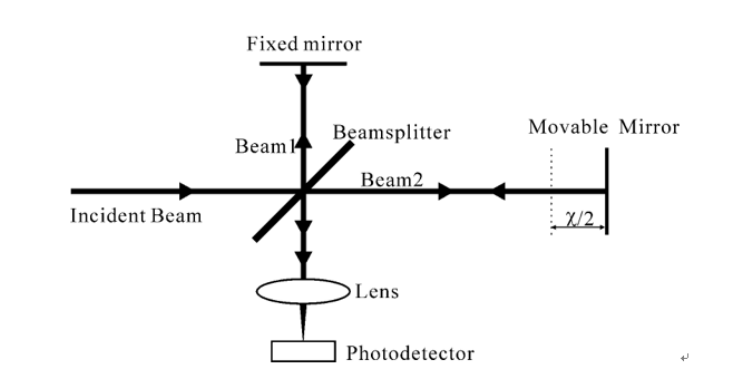
\includegraphics[width=0.5\textwidth]{pic1.PNG}}
    \caption{傅里叶变换光谱原理}
    \label{pic1}
\end{figure}

\subsection{单色光的情况}
假设来自分束器的两束光的强度比为 1 : 1, 当光源为单色光时, 两束光干涉图的强度与光程差的函数为:
\begin{align}
    I(x) = I_0\left[1 + cos (2𝜋\sigma_0 x)\right] 
\end{align}
其中$\sigma_0$为入射光的波数, $x$为光程差。

\subsection{多色光的情况}
当光源为多色光时, 多束光干涉图的强度与光程差的函数为:
\begin{align}
    I(x)=\int_{0}^{\infty} B(\sigma) \cos (2 \pi \sigma x) \mathrm{d} \sigma
\end{align}
通过构造一个$B(\sigma)$的偶函数$B_{e}(\sigma)$可以进一步得到
\begin{align}
    B_{e}(\sigma)=\int_{-\infty}^{+\infty} I(x) e^{-2 \pi \sigma x} \mathrm{~d} \sigma
\end{align}
在实际的实验中, 光程中存在色散, 会将不对称引入到干涉图中. 因此需要引入一个相位函数$\Phi(\sigma)$,干涉图的强度与光程差的函数变为
\begin{align}
    I(x)=\int_{0}^{+\infty} B(\sigma) \cos (2 \pi \sigma x+\Phi(\sigma)) \mathrm{d} \sigma
\end{align}
同样构造$B(\sigma)$的偶函数$B_{re}(\sigma)$与奇函数$B_{io}(\sigma)$得到
\begin{align*}
I(x)=\int_{-\infty}^{+\infty}\left[B_{r e}(\sigma)+i B_{i o}(\sigma)\right] e^{i 2 \pi \sigma x} \mathrm{~d} \sigma
\end{align*}
那么叠加谱为
\begin{align}
    B_{c}(\sigma)=B_{r e}(\sigma)+i B_{i o}(\sigma)=\int_{-\infty}^{+\infty} I(x) e^{-i 2 \pi \sigma x} \mathrm{~d} x 
\end{align}

\section{实验结果}
\subsection{仿真两不同频率正弦波的差拍波形}
本实验所用两个波形为$x_1(t) = 10sin500t$与$x_2(t)=20sin550t$,实验代码如下:
{%\setmonofont[Mapping={}]{Consolas}
\begin{lstlisting}[language=matlab]
 t=0:0.0001:0.5;
 A1=10;
 A2=20;
 y1=A1*sin(500*t);
 y2=A2*sin(550*t);
 y=y1+y2;
 subplot(3,1,1);
 plot(t,y1,'r.‐','LineWidth',0.5);
 title('10*sin(500*t)');
 subplot(3,1,2);
 plot(t,y2,'b.‐','LineWidth',0.5);
 title('20*sin(550*t)');
 subplot(3,1,3);
 plot(t,y,'b.‐','LineWidth',0.5);
 title('10*sin(500*t)+20*sin(550*t)');
\end{lstlisting}
}
当同方向的两个频率相差不大的简谐波叠加时, 叠加后的波形的幅值将随时间作强弱的周期性度化, 这种现象称之为“拍”. 幅值出现忽强忽弱的变化, 单位时间内出现的拍数称为拍频 (拍的频率), 也是叠加后波形的幅值变化频率.从图\ref{pic2}中可以看出, 这两个波形叠加后, 出现了 “拍” 现象。
\begin{figure}[htbp]
    \centerline{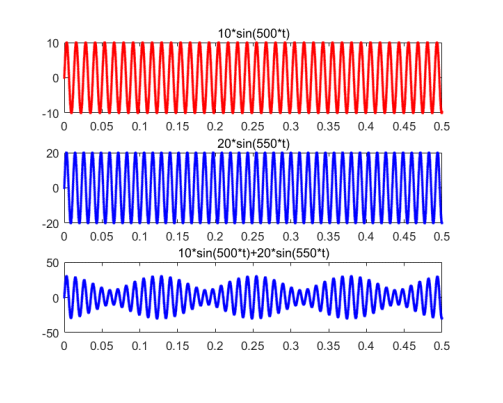
\includegraphics[width=0.5\textwidth]{pic2.PNG}}
    \caption{两不同频率正弦波的差拍波形}
    \label{pic2}
\end{figure}

\subsection{仿真单纵模 (单频) 激光输入 FTS 时, 所获得的干涉图波形}
本次实验所用两个激光波长为532nm与632.8nm。实验代码如下
{%\setmonofont[Mapping={}]{Consolas}
\begin{lstlisting}[language=matlab]
 % 波长
 lambda0=532*10^(-9);
 lambda1=632.8*10^(-9);
 % 光程差
 x=0:lambda0/100:5*lambda0;
 % 波数
 sigma0=1/lambda0;
 sigma1=1/lambda1;
 % 干涉谱
 I0=1*(1+cos(2*pi*sigma0*x));
 I1=1*(1+cos(2*pi*sigma1*x));
 I3=I1+I0;
 % 画图
 subplot(3,1,1)
 plot(x,I0,'r.-','LineWidth',0.5)
 axis([0 2.5*10^(-6) 0 2])
 title('532nm')
 subplot(3,1,2)
 plot(x,I1,'b.-','LineWidth',0.5)
 axis([0 2.5*10^(-6) 0 2])
 title('632.8nm')
 subplot(3,1,3)
 plot(x,I3,'b.-','LineWidth',0.5)
 axis([0 2.5*10^(-6) 0 4])
 title('532nm+632.8nm')
\end{lstlisting}}

实验所作两个单色光干涉图如图\ref{pic3}所示。
\begin{figure}[htbp]
    \centerline{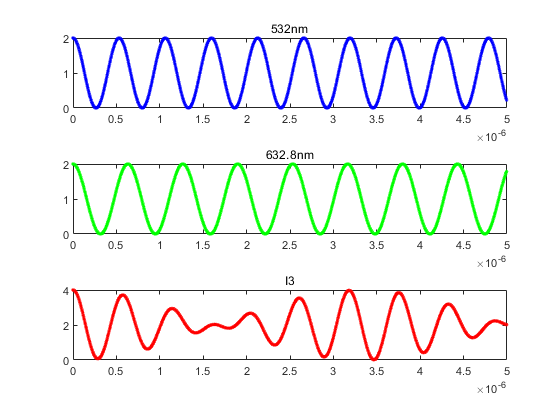
\includegraphics[width=0.5\textwidth]{pic3.png}}
    \caption{单纵模 (单频) 激光输入 FTS 所获得的干涉图波形}
    \label{pic3}
\end{figure}

\subsection{仿真非单纵模(多频)激光输入FTS时, 所获得的干涉图波形}
本实验激光中心波长选 532nm 和 632.8nm, 频间隔300MHz。
实验代码如下:
{%\setmonofont[Mapping={}]{Consolas}
\begin{lstlisting}[language=matlab]
 clc;
 clear;
 close all;
 % 波长为632.8nm
 % lambda=632.8*10^(-9);
 lambda=532*10^(-9);
 % 光程差
 x=0:lambda/10:2;
 % 光速
 c=3*10^8;
 % 632.8nm波长对应的频率
 f=c/lambda;
 % 频间隔为300MHz
 delta_f=300*10^6;
 % 幅度
 I=1;
 % 设置不同频率
 f0=f;
 f1=f-delta_f;
 f2=f+delta_f;
 f3=f-2*delta_f;
 f4=f+2*delta_f;
 f5=f-3*delta_f;
 f6=f+3*delta_f;
 % 不同频率对应的波长
 lambda0=c/f0;
 lambda1=c/f1;
 lambda2=c/f2;
 lambda3=c/f3;
 lambda4=c/f4;
 lambda5=c/f5;
 lambda6=c/f6;
 % 不同频率对应的波数
 sigma0=1/lambda0;
 sigma1=1/lambda1;
 sigma2=1/lambda2;
 sigma3=1/lambda3;
 sigma4=1/lambda4;
 sigma5=1/lambda5;
 sigma6=1/lambda6;
 % 不同频率对应的干涉强度
 I0=(1+cos(2*pi*sigma0*x));
 I1=(1+cos(2*pi*sigma1*x));
 I2=(1+cos(2*pi*sigma2*x));
 I3=(1+cos(2*pi*sigma3*x));
 I4=(1+cos(2*pi*sigma4*x));
 I5=(1+cos(2*pi*sigma5*x));
 I6=(1+cos(2*pi*sigma6*x));
 % 将3个不同频率、5个不同频率和7个不同频率的干涉图相加
 IA=I0+I1+I2;
 IB=I0+I1+I2+I3+I4;
 IC=I0+I1+I2+I3+I4+I5+I6;
 % 画图
 figure;
 subplot(2,1,1);
 plot(x,IA,'r.-','LineWidth',0.5);
 title('532nm-3个频率干涉');
 subplot(2,1,2);
 plot(x,IB,'b.-','LineWidth',0.5);
 title('532nm-5个频率干涉');
 subplot(3,1,3);
 plot(x,IC,'r.-','LineWidth',0.5);
 title('532nm-7个频率干涉');
    
\end{lstlisting}}   
图\ref{pic4}显示了多个干涉强度相同的波的叠加干涉图,具体参数为
\begin{itemize}
    \item 叠加波的频率不同
    \item 幅值相同,均为1
    \item  采样长度:[0m, 2m]
    \item 采样间隔:632.8nm/8
    \item 中心频率:c/632.8nm
    \item 频率间隔:300MHz
\end{itemize}
\begin{figure}[htbp]
    \centerline{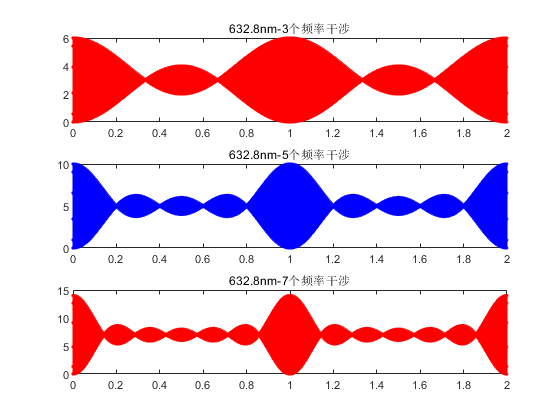
\includegraphics[width=0.5\textwidth]{pic4.png}}
    \caption{非单纵模 (多频) 激光输入FTS(情况1)}
    \label{pic4}
\end{figure}
图\ref{pic5}显示了多个干涉强度相同的波的叠加干涉图,具体参数为
\begin{itemize}
    \item 叠加波的频率不同
    \item 幅值不相同
    \item  采样长度:[0m, 2m]
    \item 采样间隔:632.8nm/8
    \item 中心频率:c/632.8nm
    \item 频率间隔:300MHz
\end{itemize}
\begin{figure}[htbp]
    \centerline{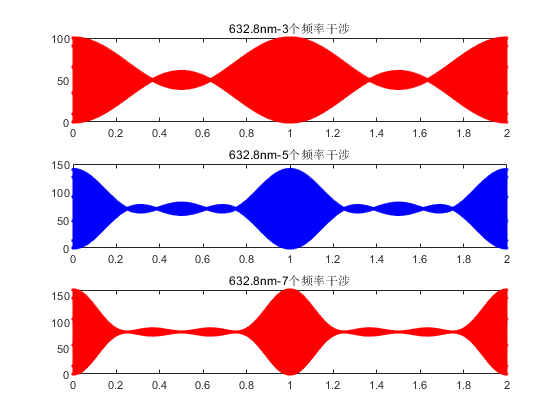
\includegraphics[width=0.5\textwidth]{pic5.png}}
    \caption{非单纵模 (多频) 激光输入FTS(情况2)}
    \label{pic5}
\end{figure}
图\ref{pic6}显示了多个干涉强度相同的波的叠加干涉图,具体参数为
\begin{itemize}
    \item 叠加波的频率不同
    \item 幅值相同,均为1
    \item  采样长度:[0m, 2m]
    \item 采样间隔:532nm/8
    \item 中心频率:c/532nm
    \item 频率间隔:300MHz
\end{itemize}
\begin{figure}[htbp]
    \centerline{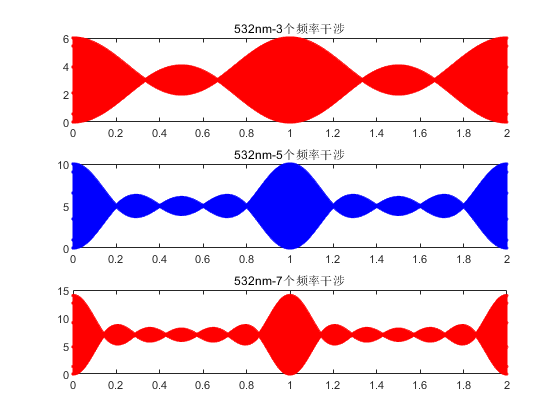
\includegraphics[width=0.5\textwidth]{pic6.png}}
    \caption{非单纵模 (多频) 激光输入FTS(情况3)}
    \label{pic6}
\end{figure}
图\ref{pic7}显示了多个干涉强度相同的波的叠加干涉图,具体参数为
\begin{itemize}
    \item 叠加波的频率不同
    \item 幅值不相同
    \item 采样长度:[0m, 2m]
    \item 采样间隔:532nm/8
    \item 中心频率:c/532nm
    \item 频率间隔:300MHz
\end{itemize}
\begin{figure}[htbp]
    \centerline{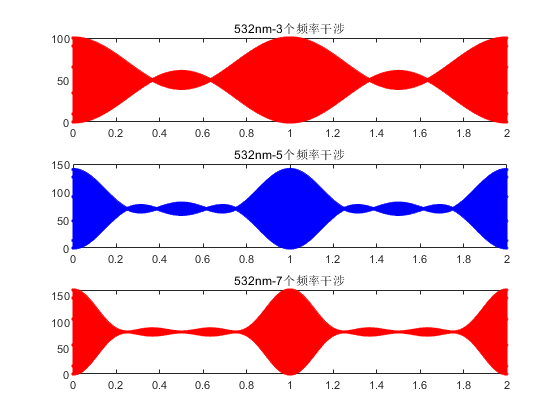
\includegraphics[width=0.5\textwidth]{pic7.png}}
    \caption{非单纵模 (多频) 激光输入FTS(情况4)}
    \label{pic7}
\end{figure}
图\ref{pic8}显示了偶数个干涉强度相同的波的叠加干涉图,具体参数为
\begin{itemize}
    \item 叠加波的频率不同
    \item 幅值相同,均为1
    \item 采样长度:[0m, 2m]
    \item 采样间隔:532nm/8
    \item 中心频率:c/532nm
    \item 频率间隔:300MHz
\end{itemize}
\begin{figure}[htbp]
    \centerline{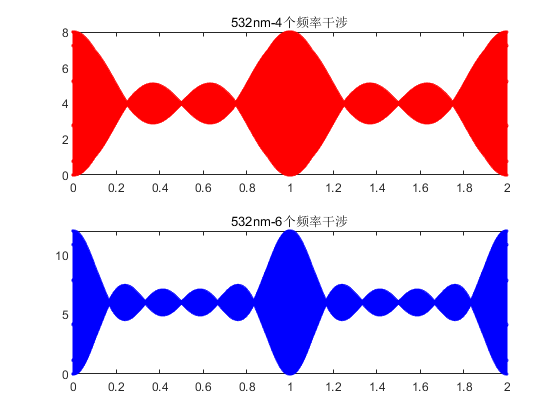
\includegraphics[width=0.5\textwidth]{pic8.png}}
    \caption{非单纵模 (多频) 激光输入FTS(情况5)}
    \label{pic8}
\end{figure}
图\ref{pic9}显示了偶数个干涉强度相同的波的叠加干涉图,具体参数为
\begin{itemize}
    \item 叠加波的频率不同
    \item 幅值不相同
    \item 采样长度:[0m, 2m]
    \item 采样间隔:532nm/8
    \item 中心频率:c/532nm
    \item 频率间隔:300MHz
\end{itemize}
\begin{figure}[htbp]
    \centerline{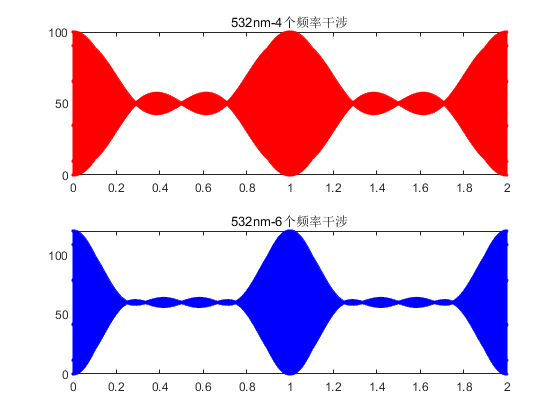
\includegraphics[width=0.5\textwidth]{pic9.png}}
    \caption{非单纵模 (多频) 激光输入FTS(情况5)}
    \label{pic9}
\end{figure}

\subsection{仿真非单纵模 (多频) 激光输入FTS时, 不同扫描长度干涉图所计算出的光谱曲线}
本实验激光中心波长选 532nm 和 632.8nm, 频间隔300MHz, 干涉图采样间隔为632.8nm/8 或 632.8nm/4。
实验代码参见附录. 

图\ref{pic10}显示了奇数个干涉强度相同的波的叠加干涉图,具体参数为
\begin{itemize}
    \item 叠加波的频率不同
    \item 幅值相同
    \item 扫描长度:1m
    \item 中心波长:532nm
    \item 采样间隔:632.8nm/4
    \item 频率间隔:300MHz
\end{itemize}
\begin{figure}[htbp]
    \centerline{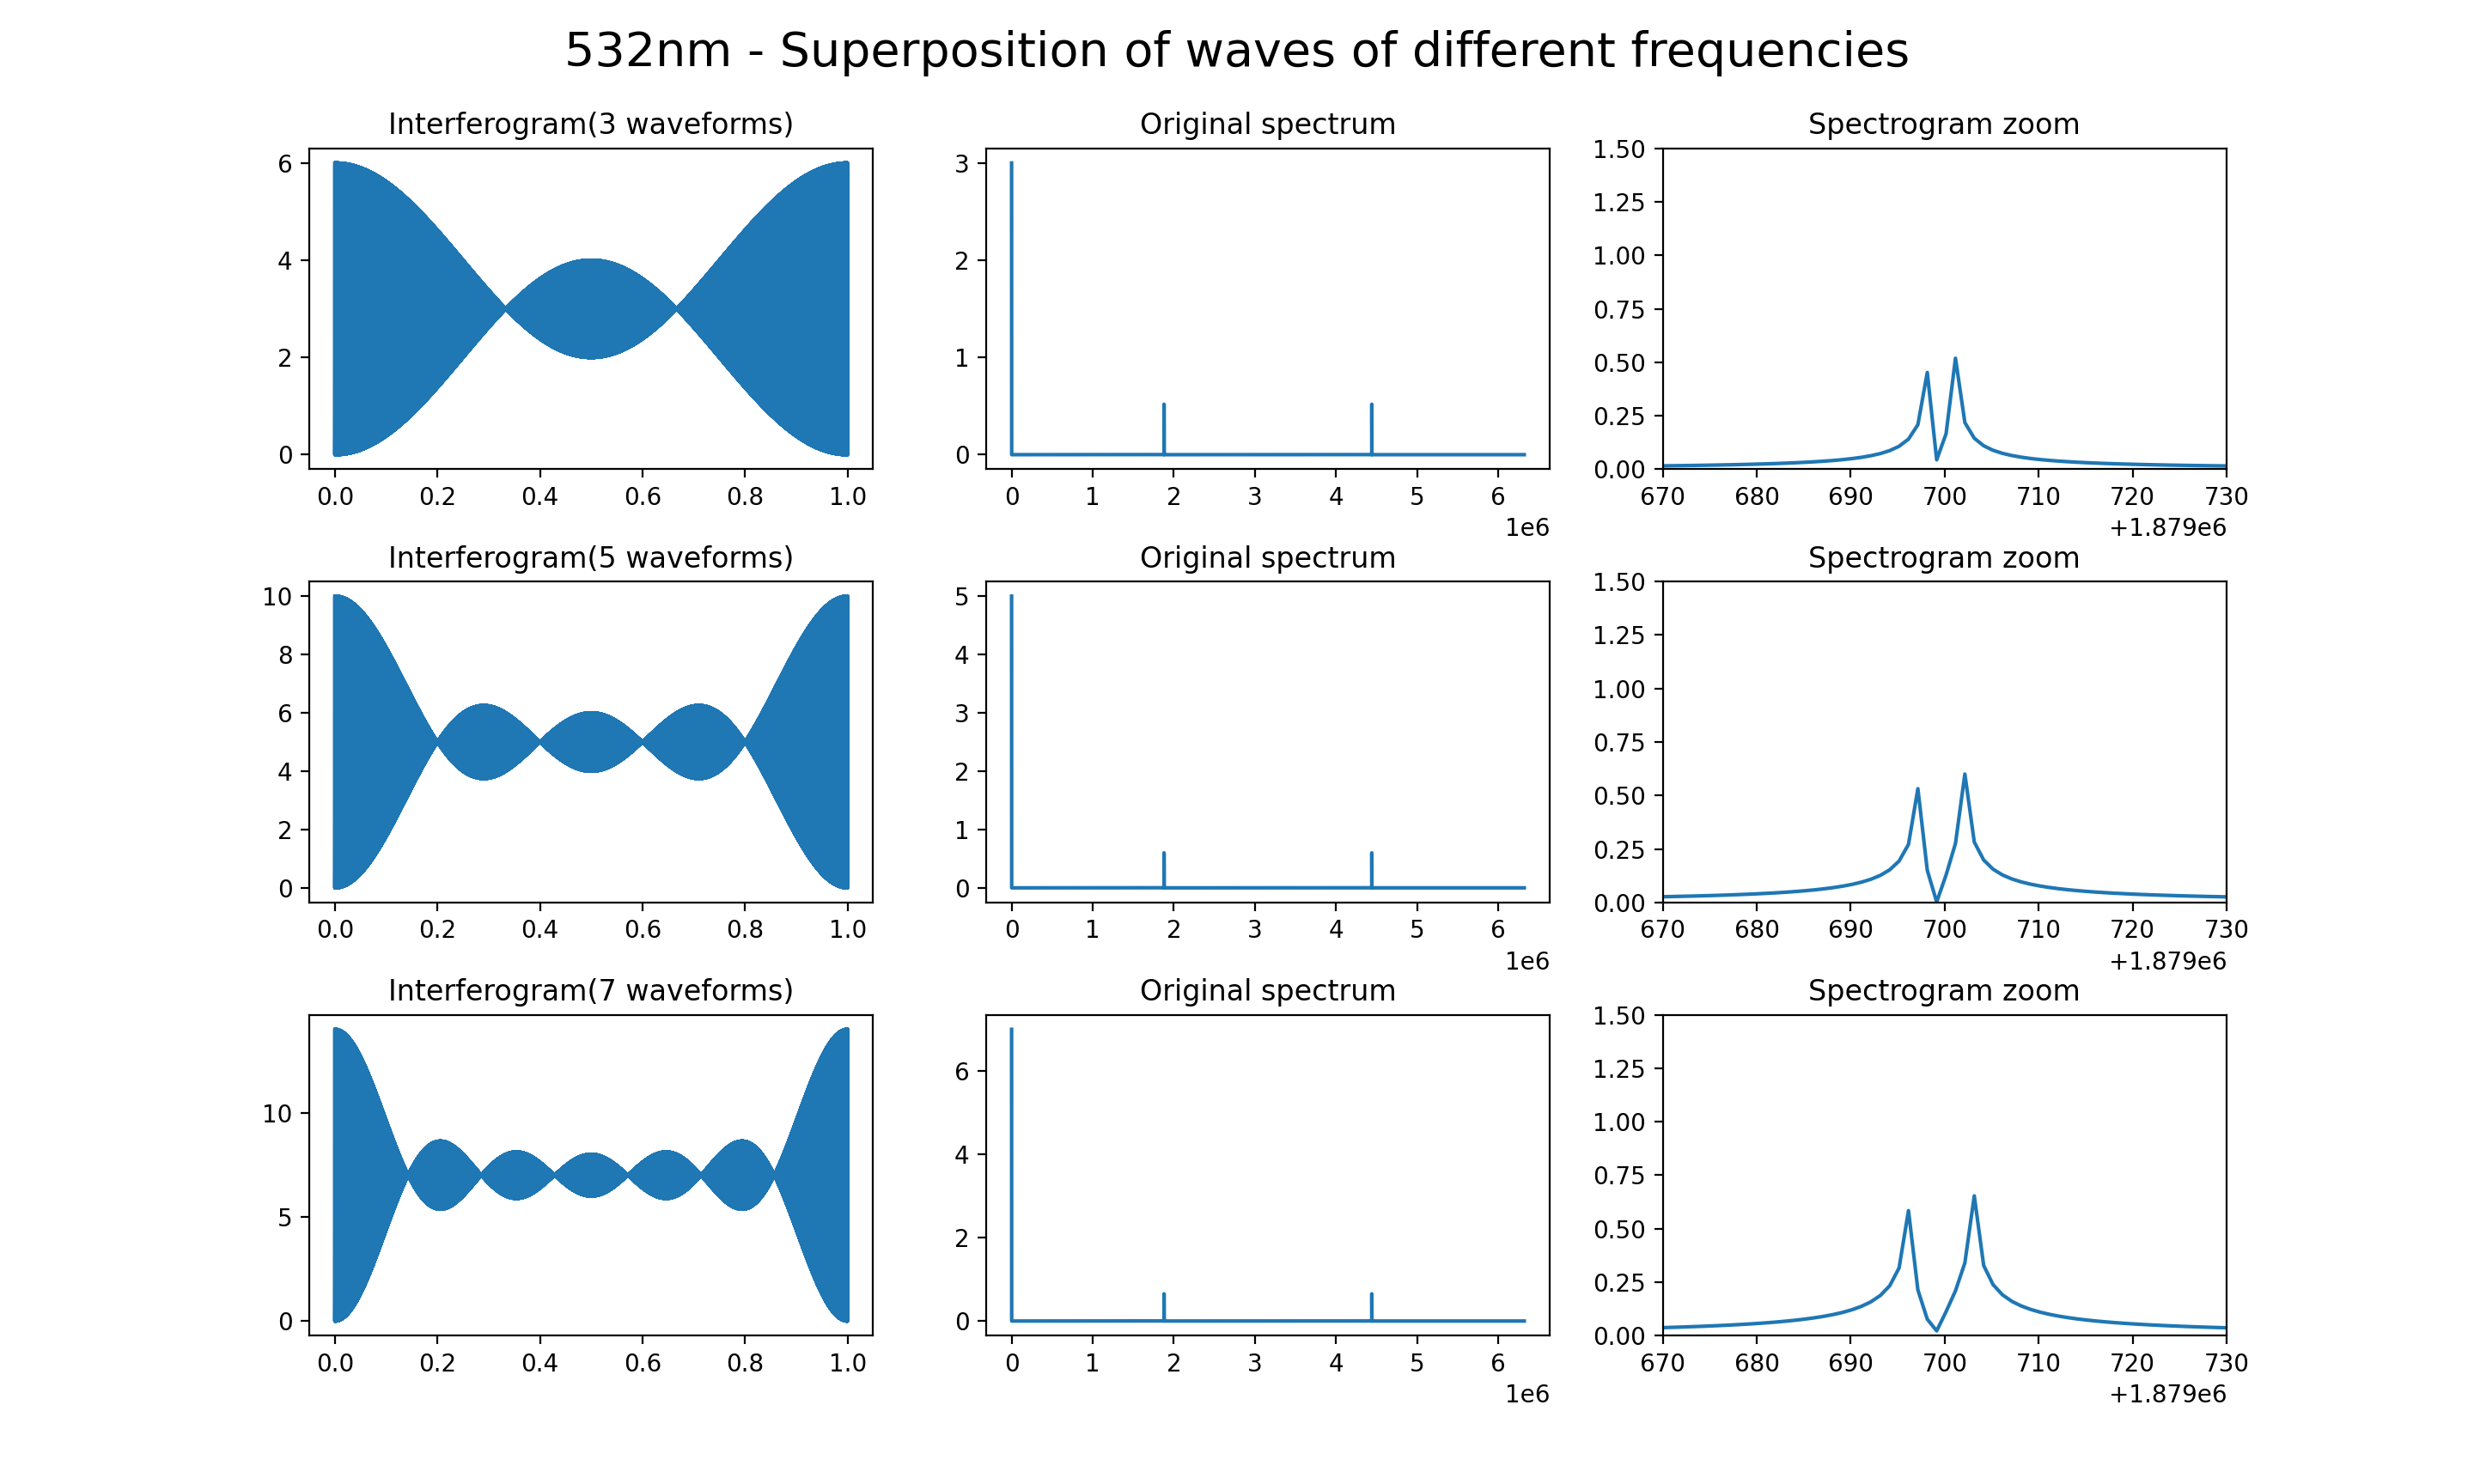
\includegraphics[width=0.5\textwidth]{pic10.png}}
    \caption{非单纵模 (多频) 激光输入FTS(情况1)}
    \label{pic10}
\end{figure}

图\ref{pic11}显示了奇数个干涉强度相同的波的叠加干涉图,具体参数为
\begin{itemize}
    \item 叠加波的频率不同
    \item 幅值相同
    \item 扫描长度:1m
    \item 中心波长:532nm
    \item 采样间隔:632.8nm/8
    \item 频率间隔:300MHz
\end{itemize}
\begin{figure}[htbp]
    \centerline{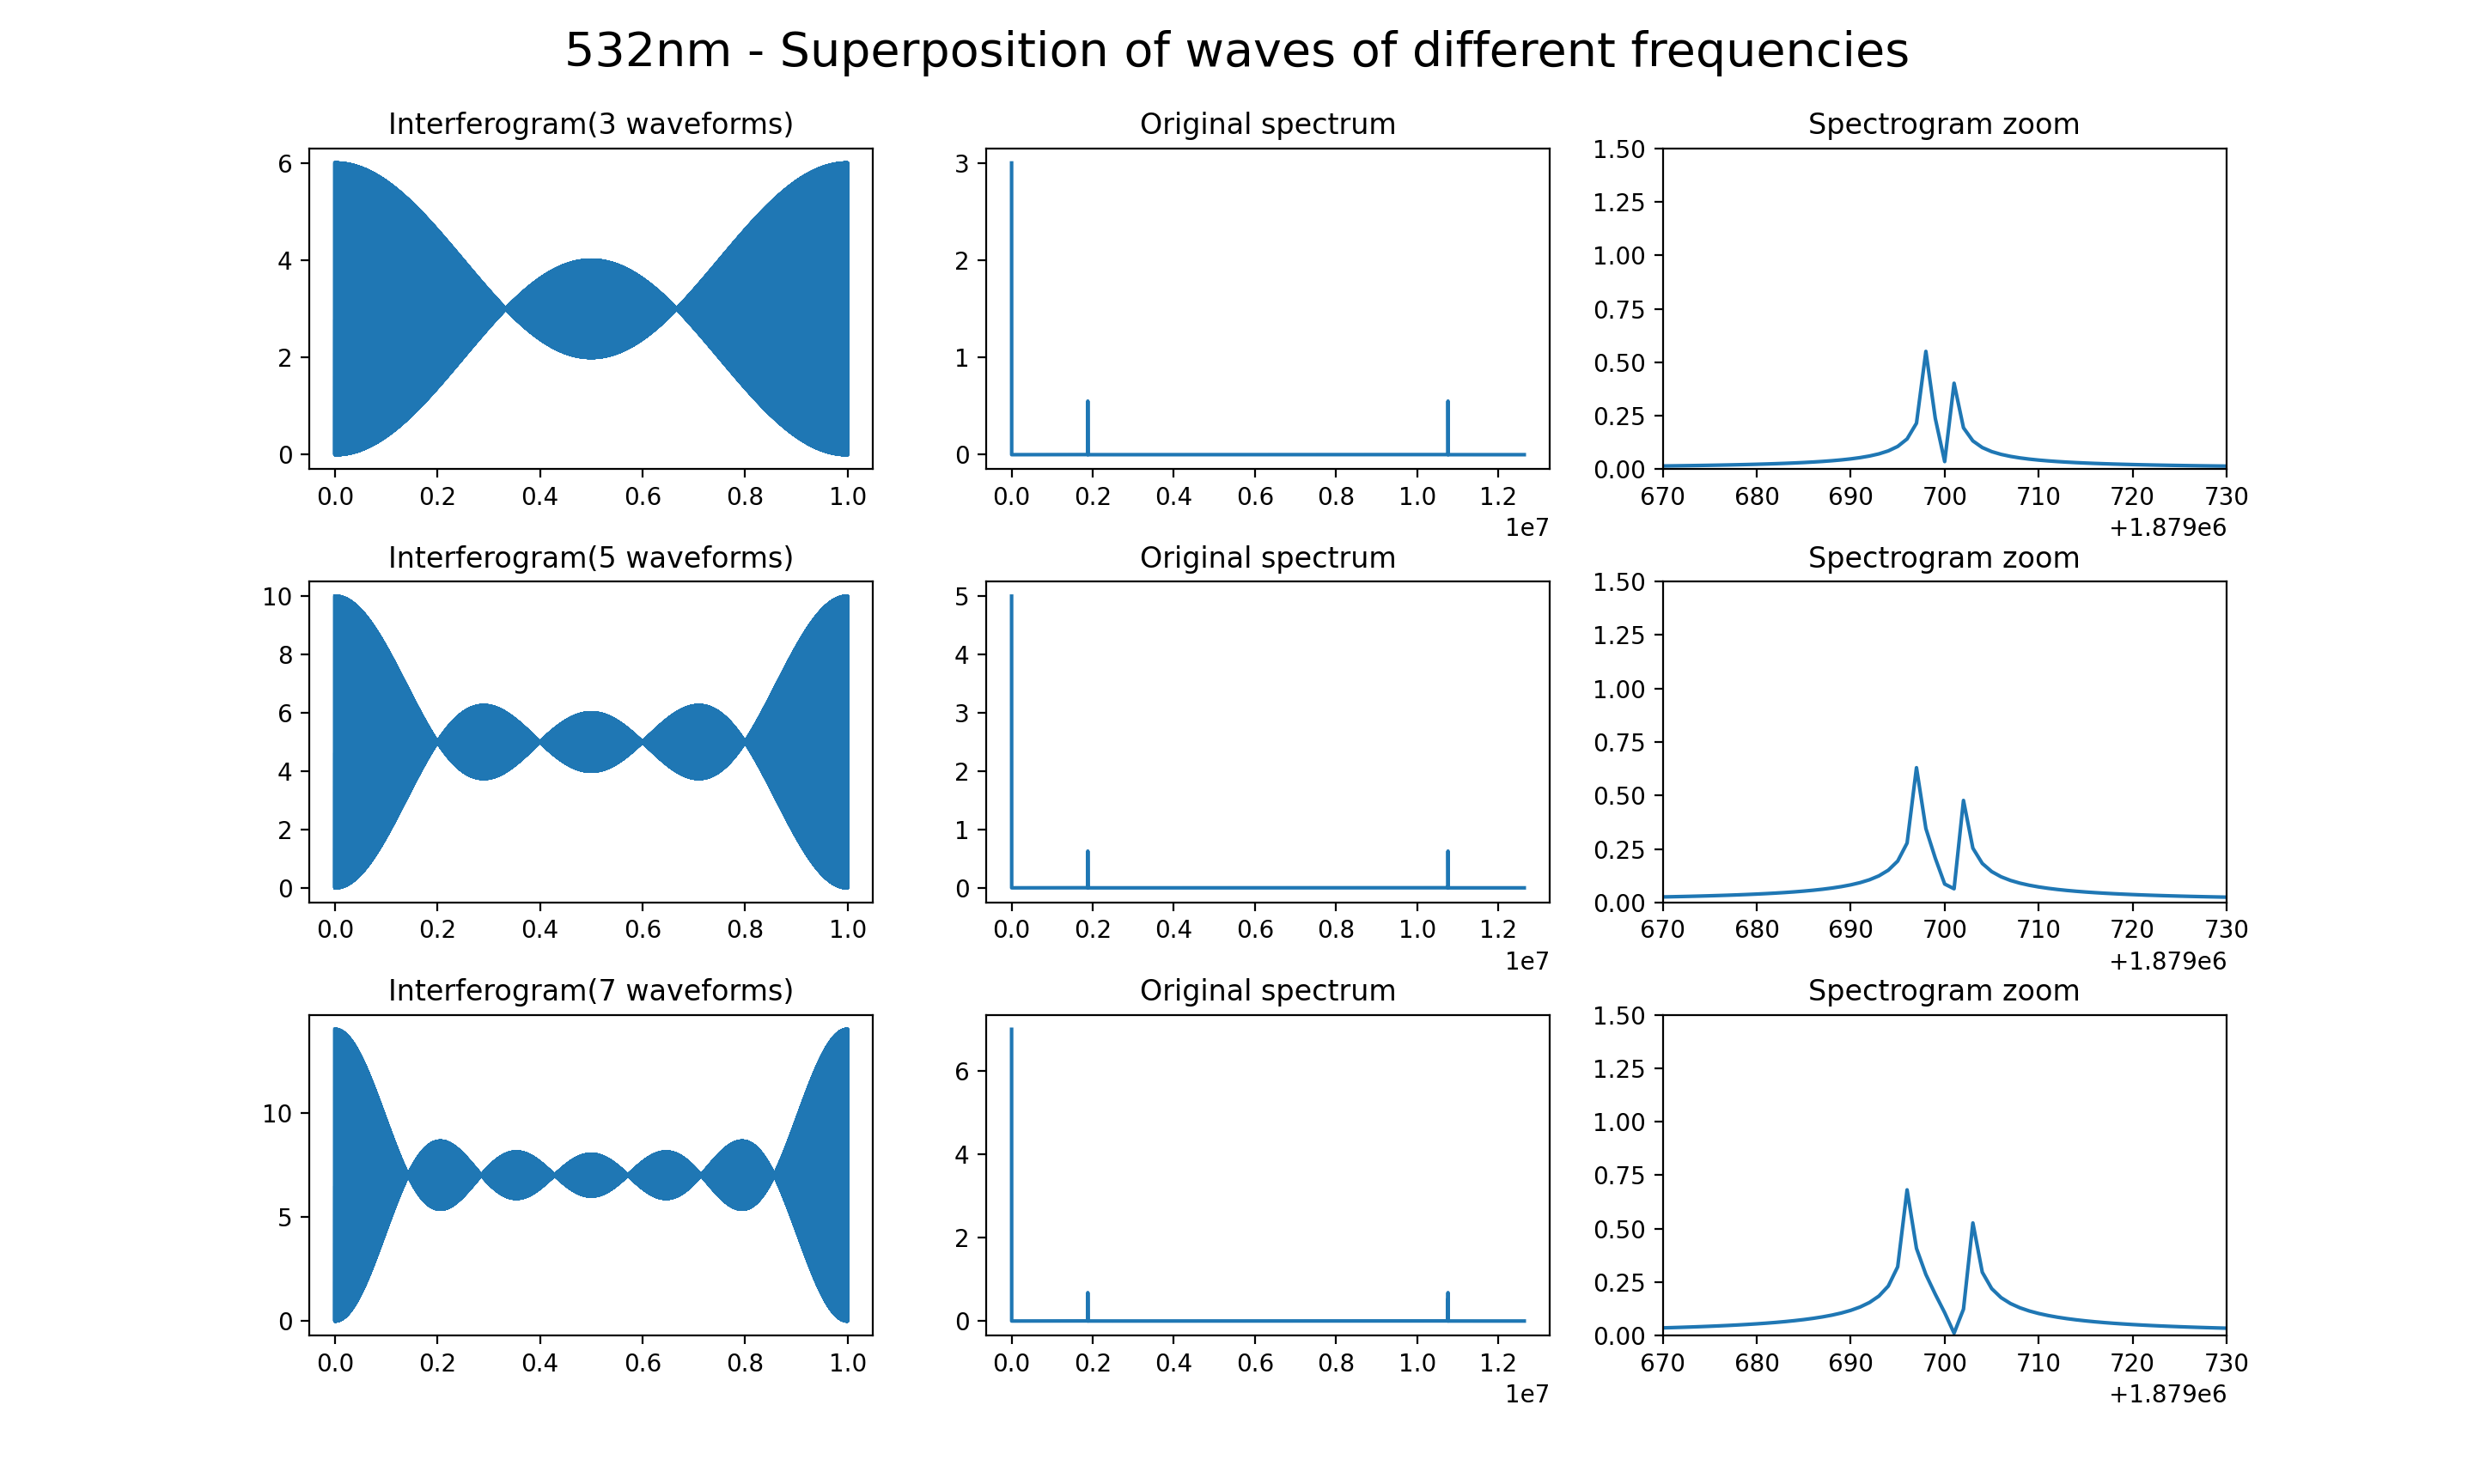
\includegraphics[width=0.5\textwidth]{pic11.png}}
    \caption{非单纵模 (多频) 激光输入FTS(情况2)}
    \label{pic11}
\end{figure}

图\ref{pic12}显示了奇数个干涉强度相同的波的叠加干涉图,具体参数为
\begin{itemize}
    \item 叠加波的频率不同
    \item 幅值不同
    \item 扫描长度:1m
    \item 中心波长:532nm
    \item 采样间隔:632.8nm/4
    \item 频率间隔:300MHz
\end{itemize}
\begin{figure}[htbp]
    \centerline{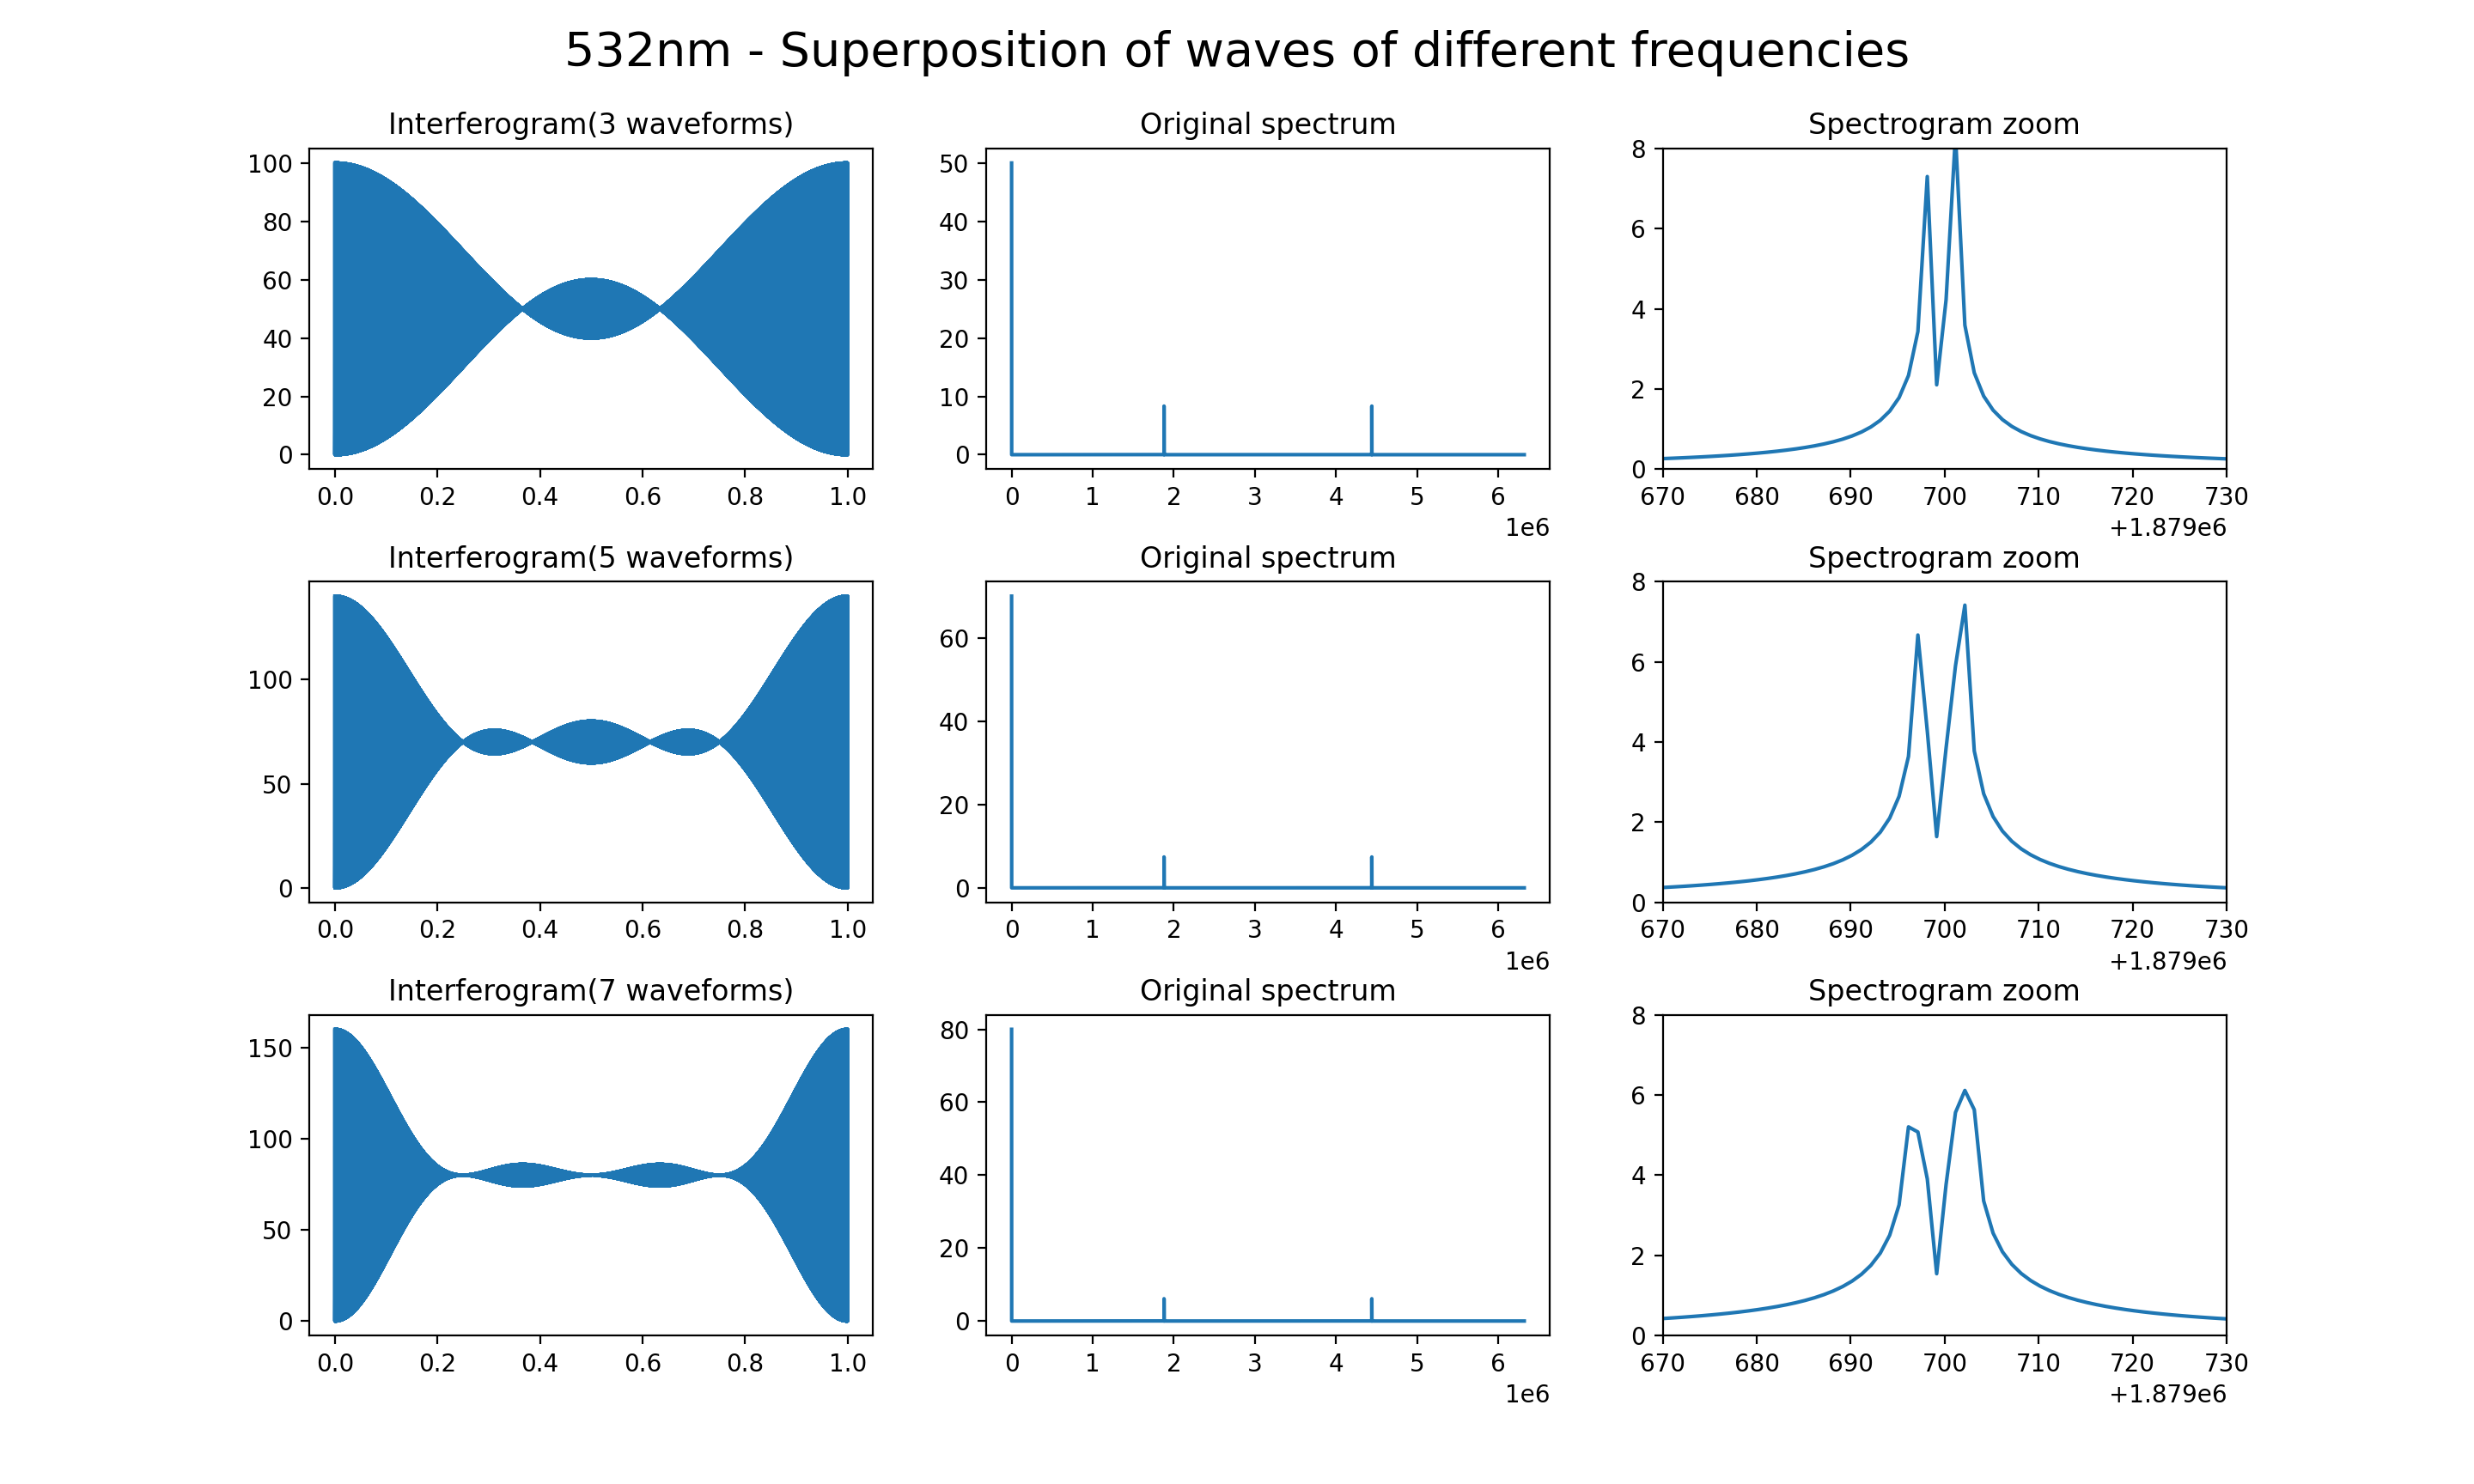
\includegraphics[width=0.5\textwidth]{pic12.png}}
    \caption{非单纵模 (多频) 激光输入FTS(情况3)}
    \label{pic12}
\end{figure}

图\ref{pic13}显示了奇数个干涉强度相同的波的叠加干涉图,具体参数为
\begin{itemize}
    \item 叠加波的频率不同
    \item 幅值不同
    \item 扫描长度:1m
    \item 中心波长:532nm
    \item 采样间隔:632.8nm/8
    \item 频率间隔:300MHz
\end{itemize}
\begin{figure}[htbp]
    \centerline{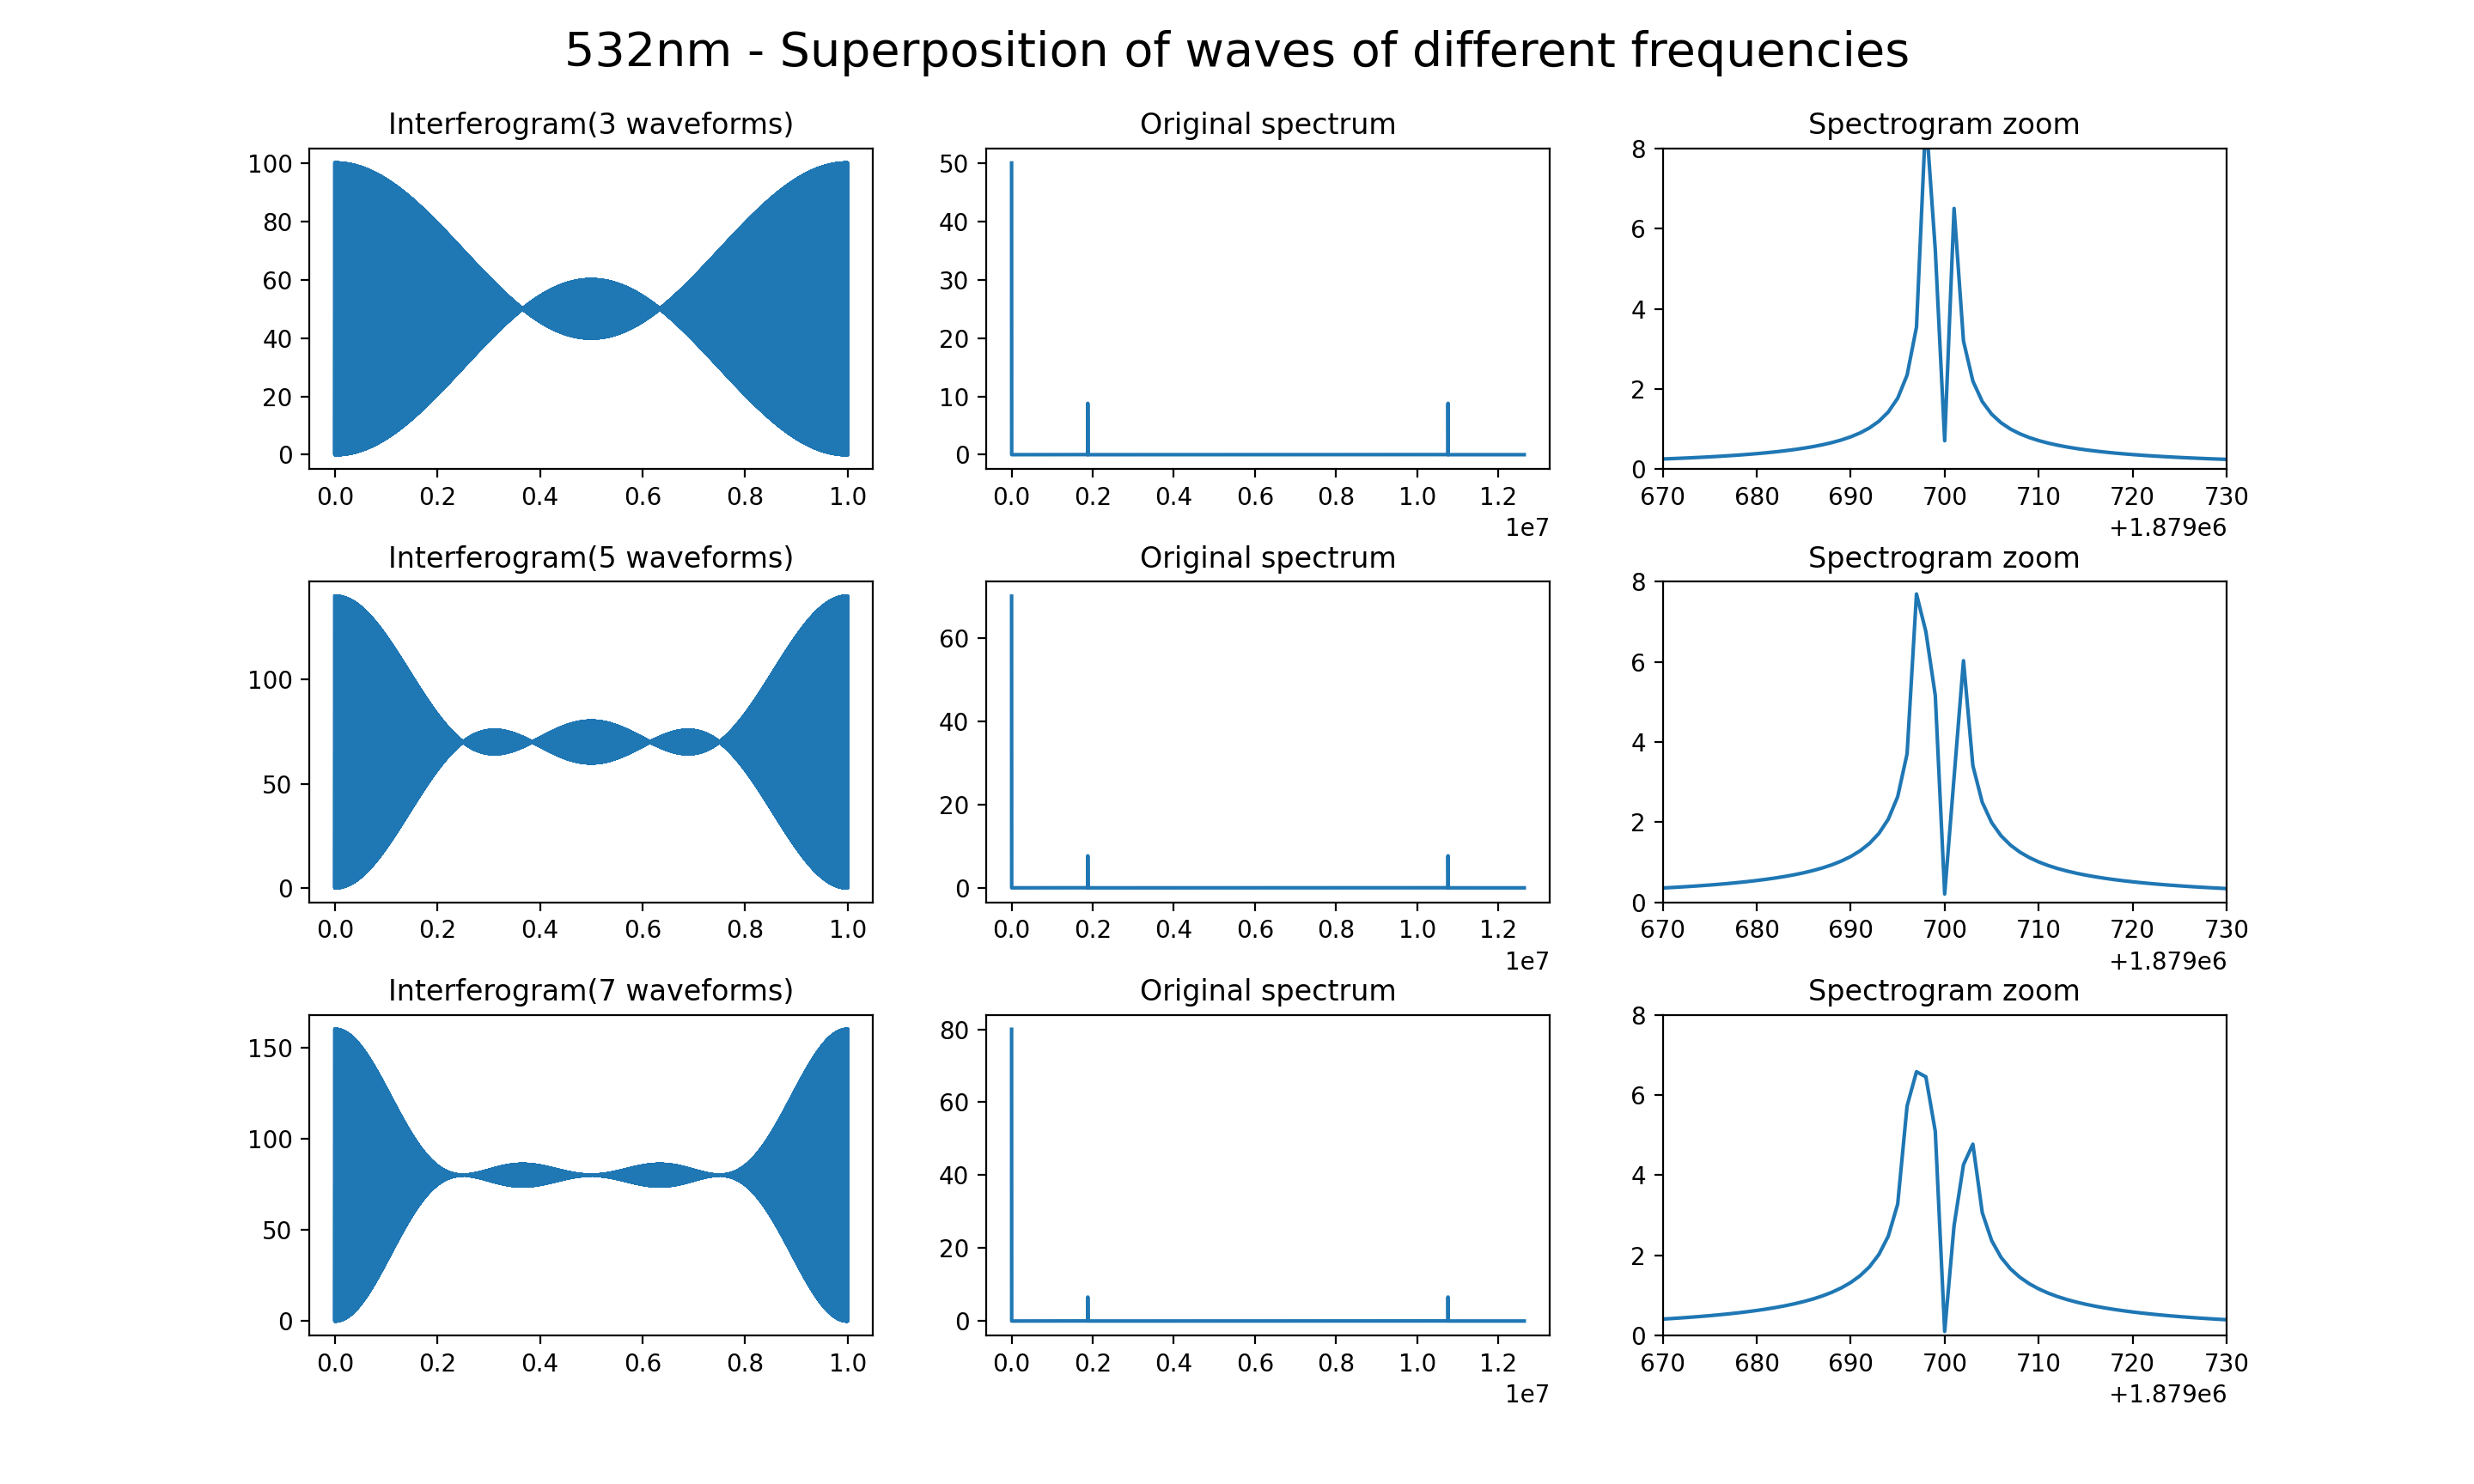
\includegraphics[width=0.5\textwidth]{pic13.png}}
    \caption{非单纵模 (多频) 激光输入FTS(情况4)}
    \label{pic13}
\end{figure}

图\ref{pic14}显示了奇数个干涉强度相同的波的叠加干涉图,具体参数为
\begin{itemize}
    \item 叠加波的频率不同
    \item 幅值相同
    \item 扫描长度:1m
    \item 中心波长:632.8nm
    \item 采样间隔:632.8nm/4
    \item 频率间隔:300MHz
\end{itemize}
\begin{figure}[htbp]
    \centerline{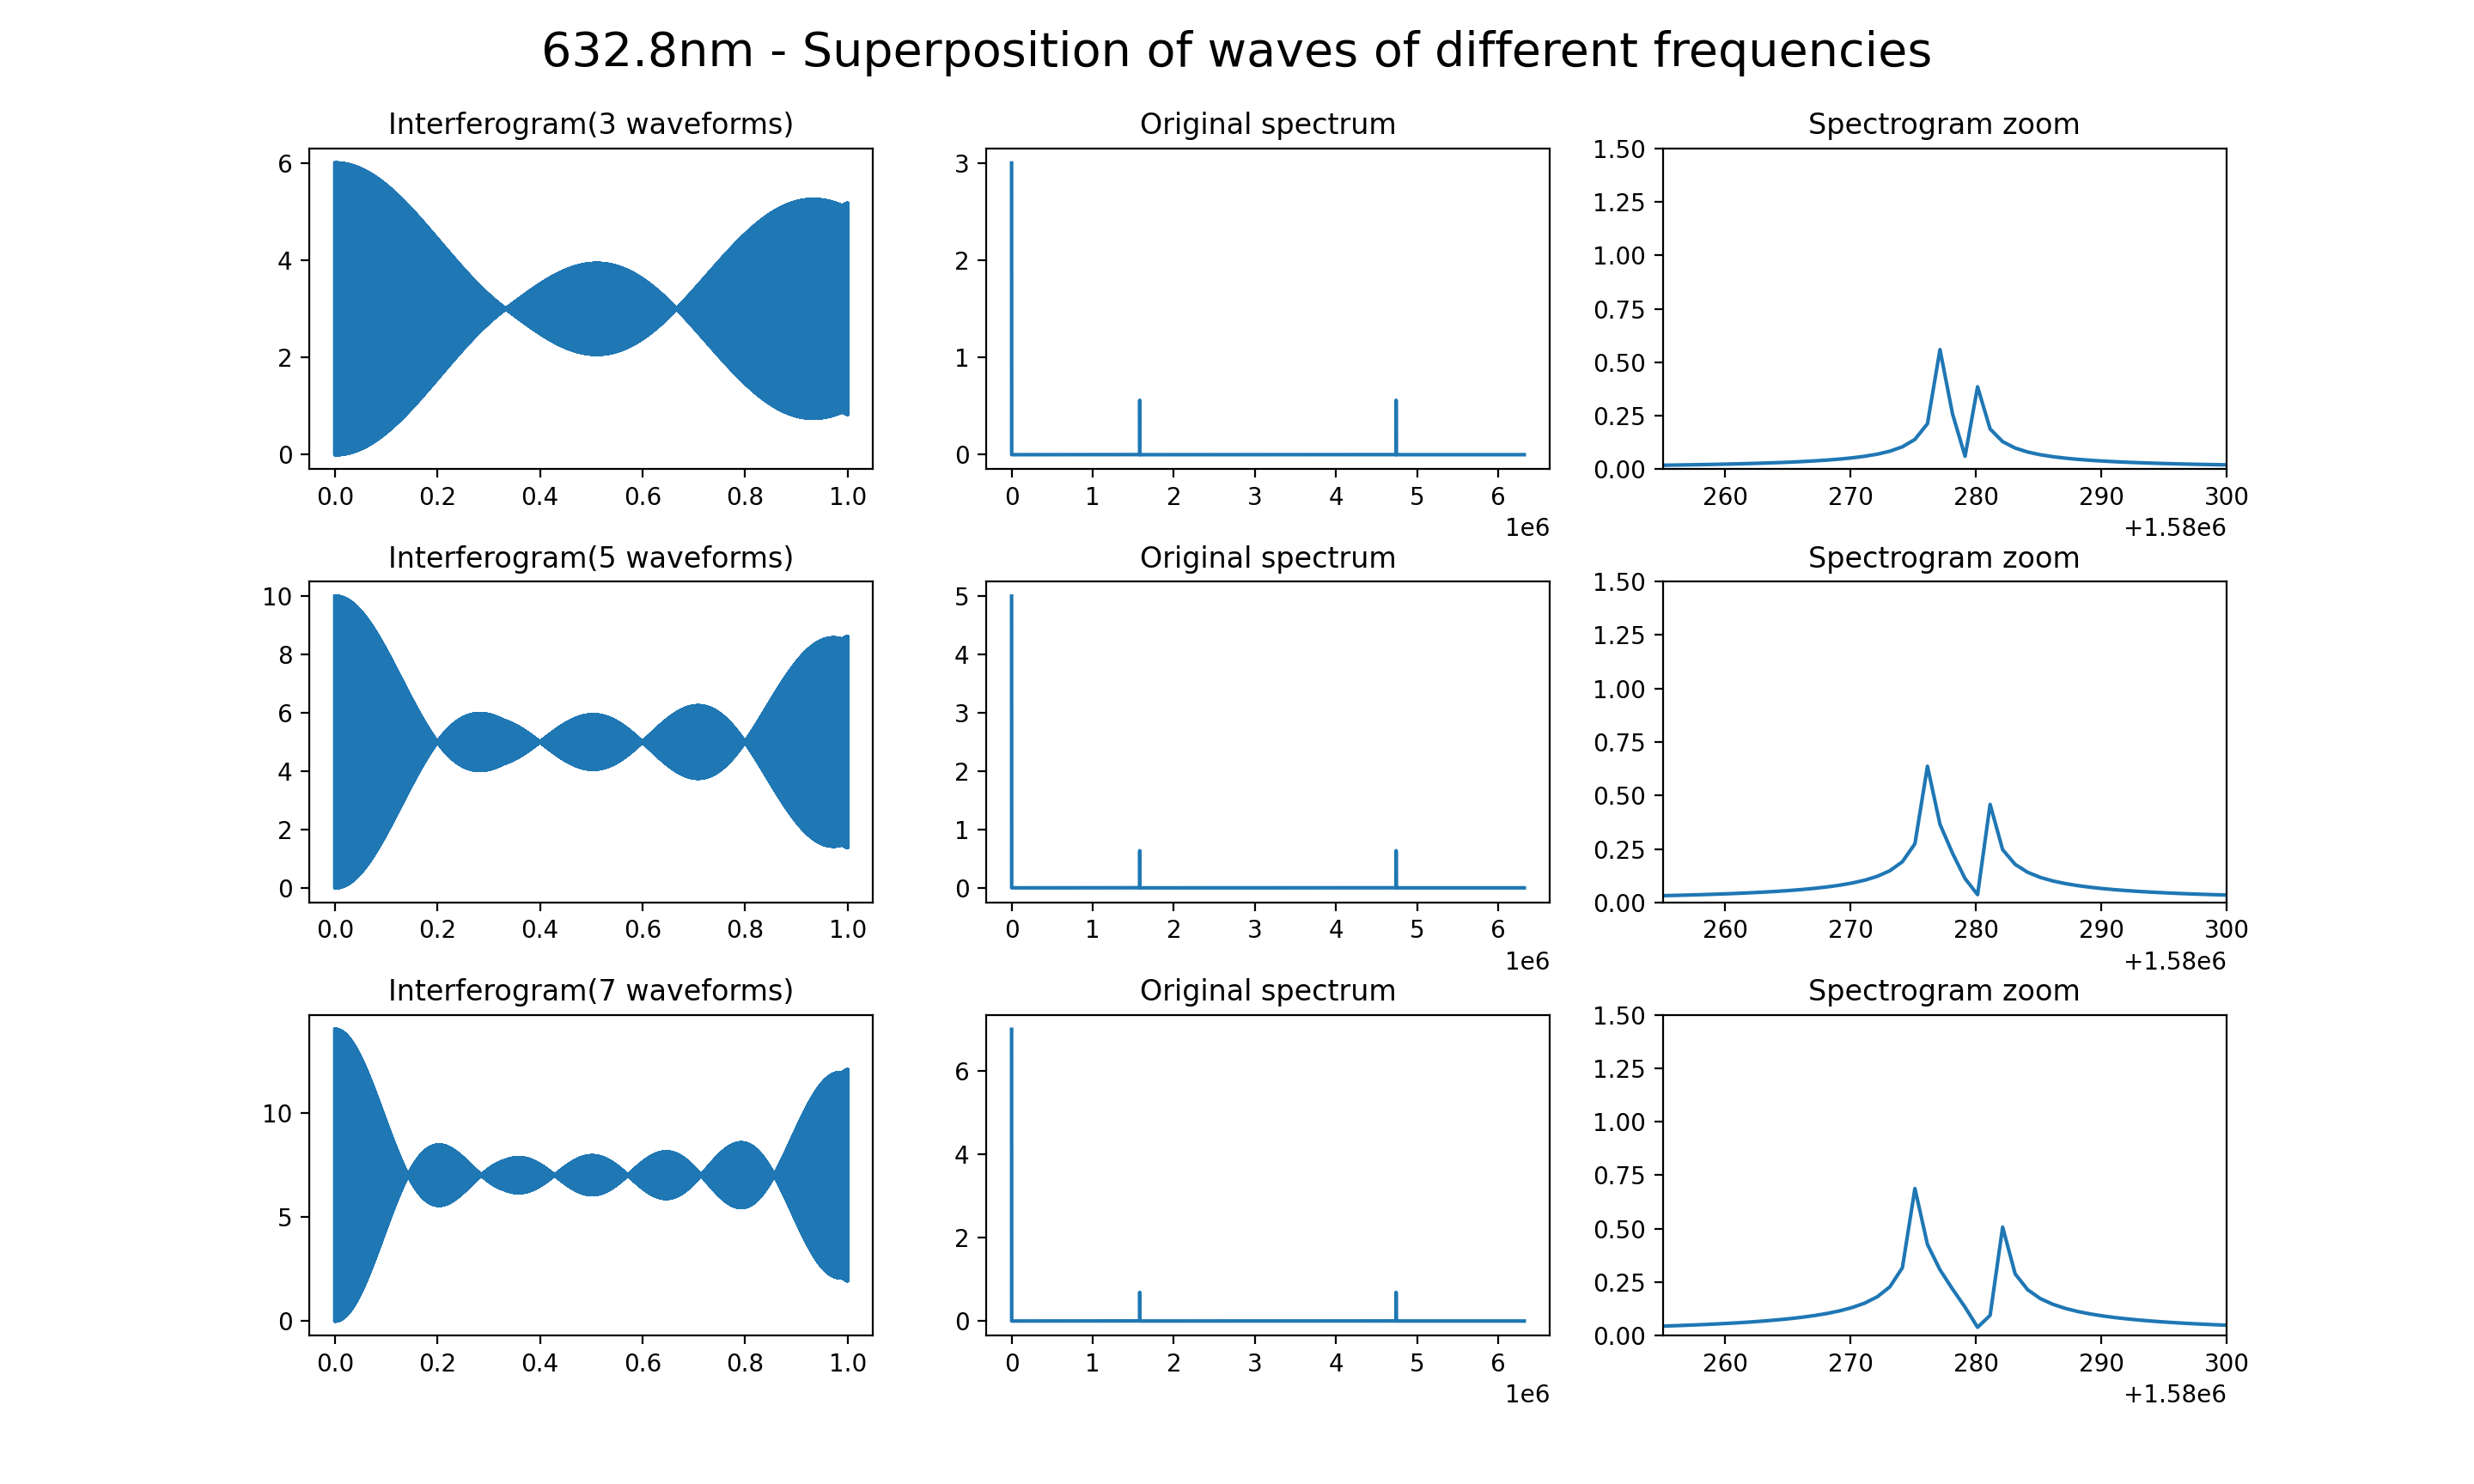
\includegraphics[width=0.5\textwidth]{pic14.png}}
    \caption{非单纵模 (多频) 激光输入FTS(情况5)}
    \label{pic14}
\end{figure}


图\ref{pic15}显示了奇数个干涉强度相同的波的叠加干涉图,具体参数为
\begin{itemize}
    \item 叠加波的频率不同
    \item 幅值不相同
    \item 扫描长度:1m
    \item 中心波长:632.8nm
    \item 采样间隔:632.8nm/4
    \item 频率间隔:300MHz
\end{itemize}
\begin{figure}[htbp]
    \centerline{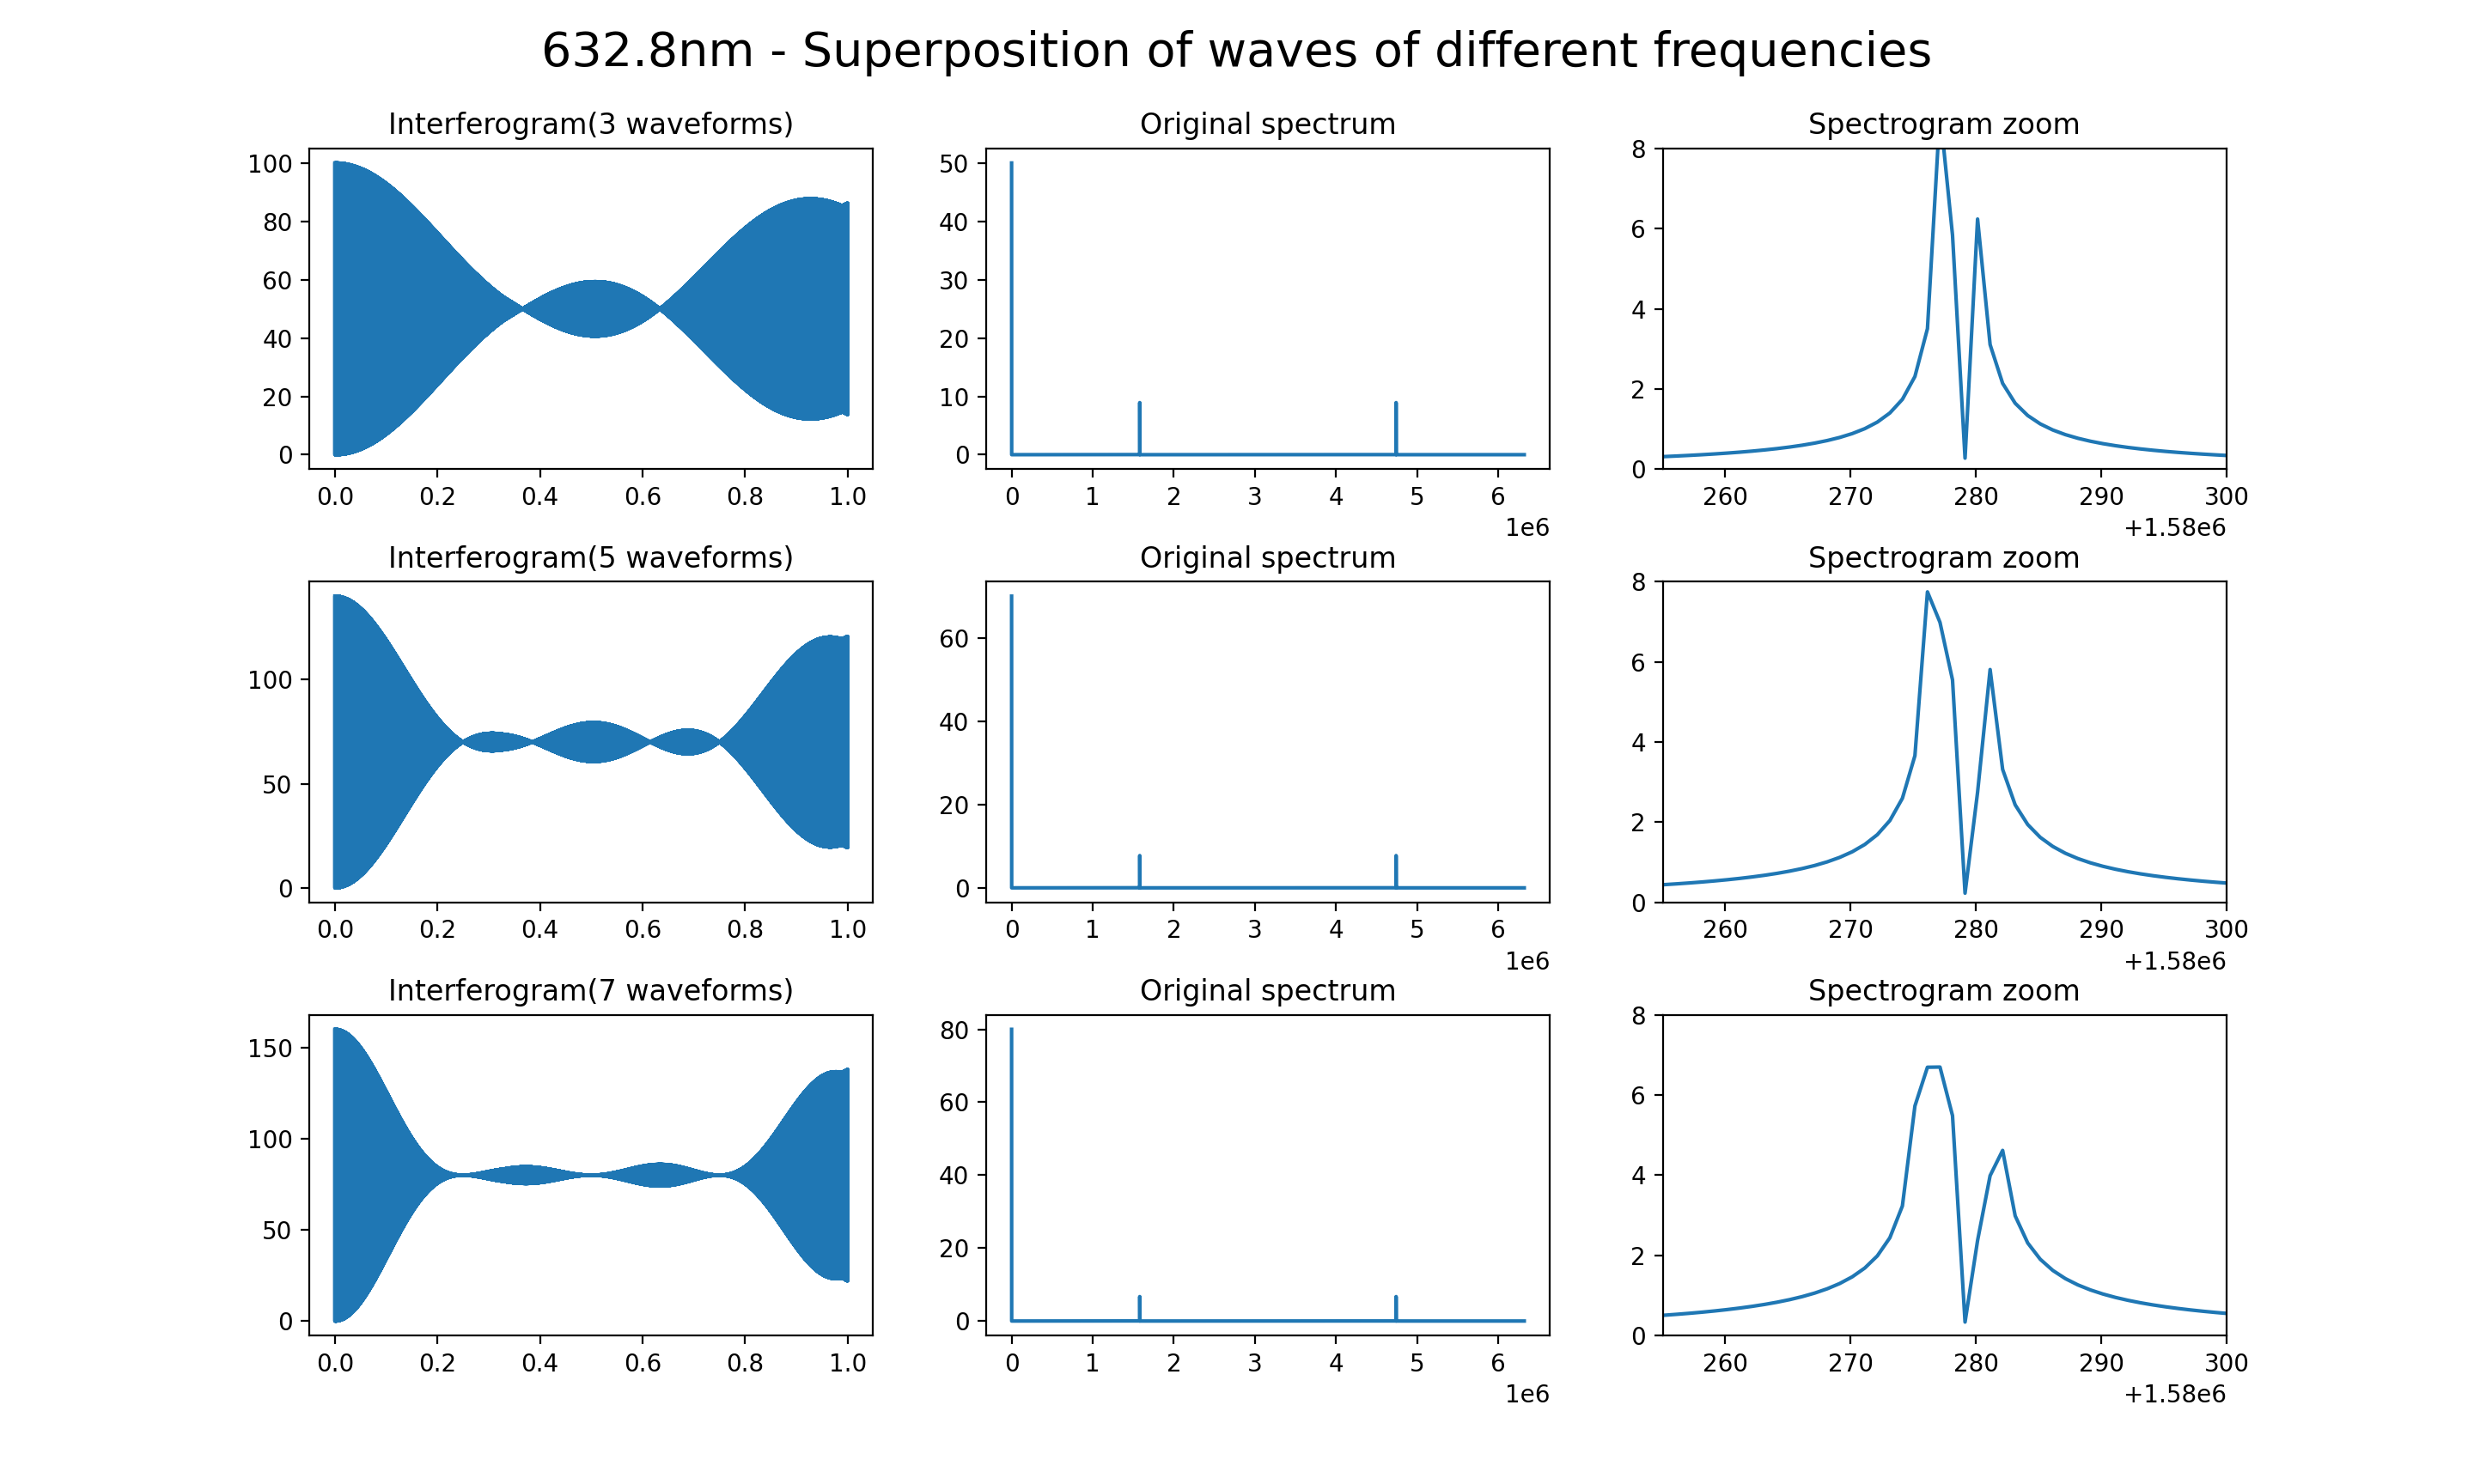
\includegraphics[width=0.5\textwidth]{pic15.png}}
    \caption{非单纵模 (多频) 激光输入FTS(情况6)}
    \label{pic15}
\end{figure}

图\ref{pic16}显示了奇数个干涉强度相同的波的叠加干涉图,具体参数为
\begin{itemize}
    \item 叠加波的频率不同
    \item 幅值相同
    \item 扫描长度:1m
    \item 中心波长:632.8nm
    \item 采样间隔:632.8nm/8
    \item 频率间隔:300MHz
\end{itemize}
\begin{figure}[htbp]
    \centerline{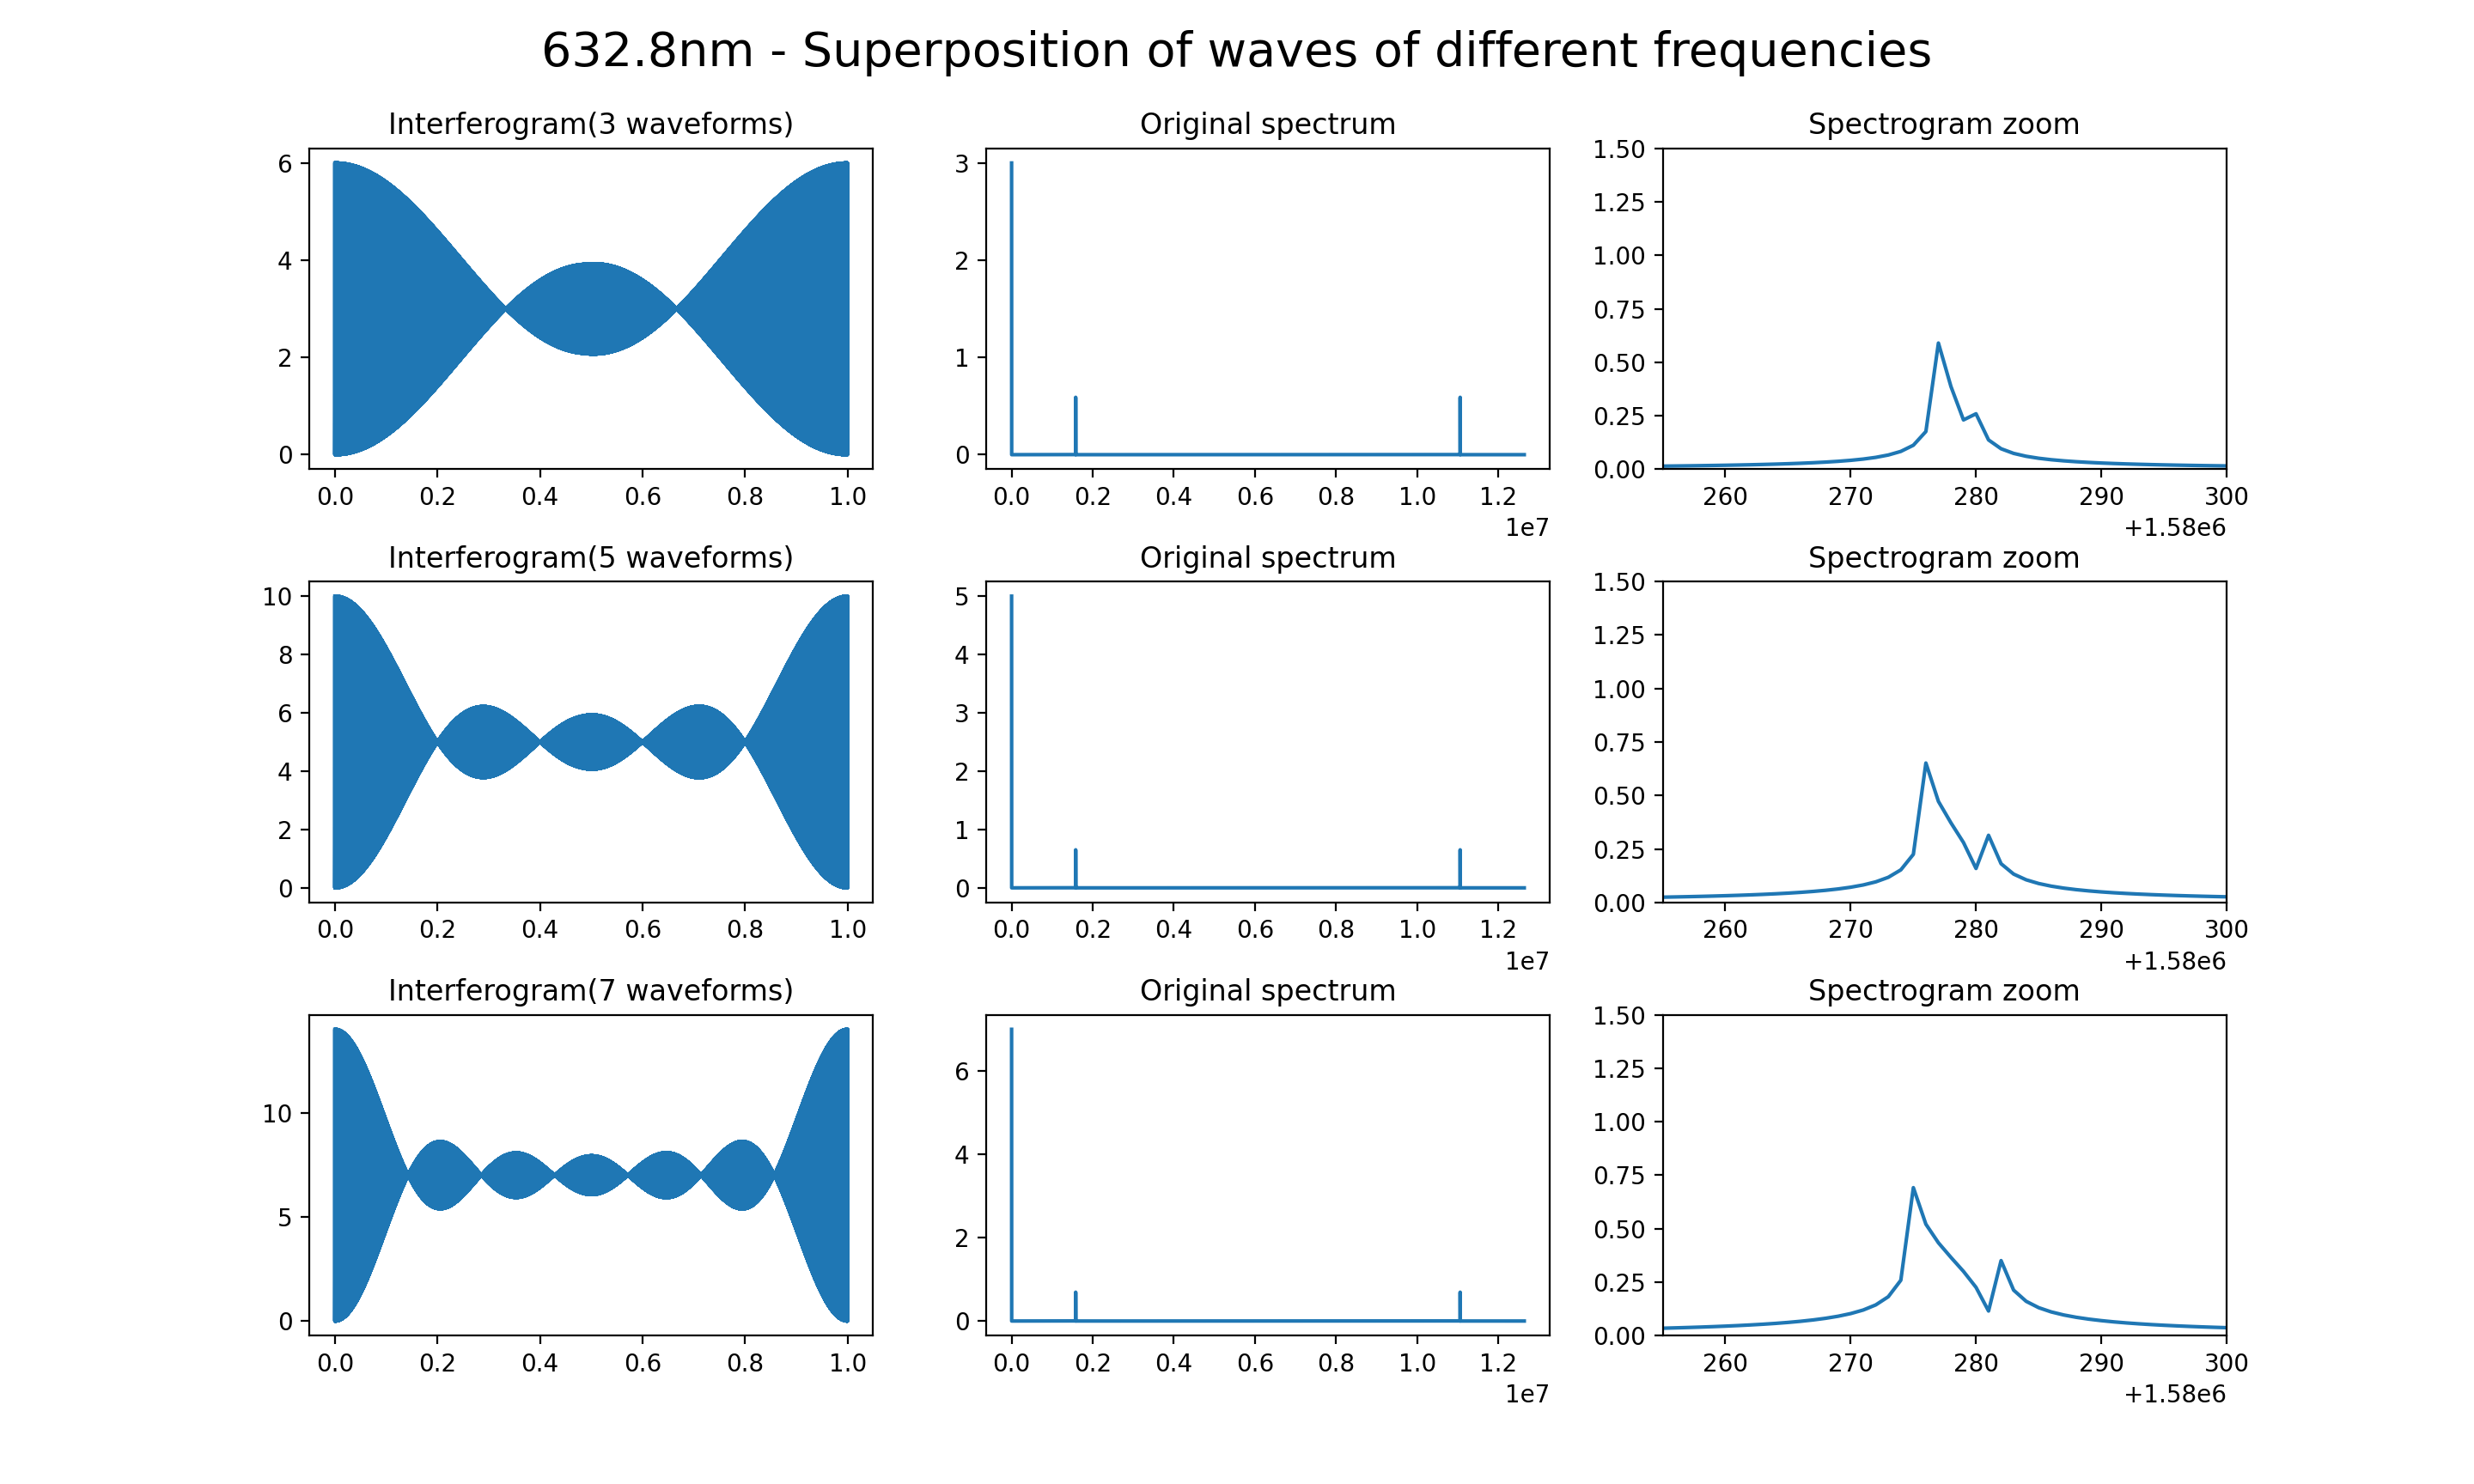
\includegraphics[width=0.5\textwidth]{pic16.png}}
    \caption{非单纵模 (多频) 激光输入FTS(情况7)}
    \label{pic16}
\end{figure}

图\ref{pic17}显示了奇数个干涉强度相同的波的叠加干涉图,具体参数为
\begin{itemize}
    \item 叠加波的频率不同
    \item 幅值不相同
    \item 扫描长度:1m
    \item 中心波长:632.8nm
    \item 采样间隔:632.8nm/8
    \item 频率间隔:300MHz
\end{itemize}
\begin{figure}[htbp]
    \centerline{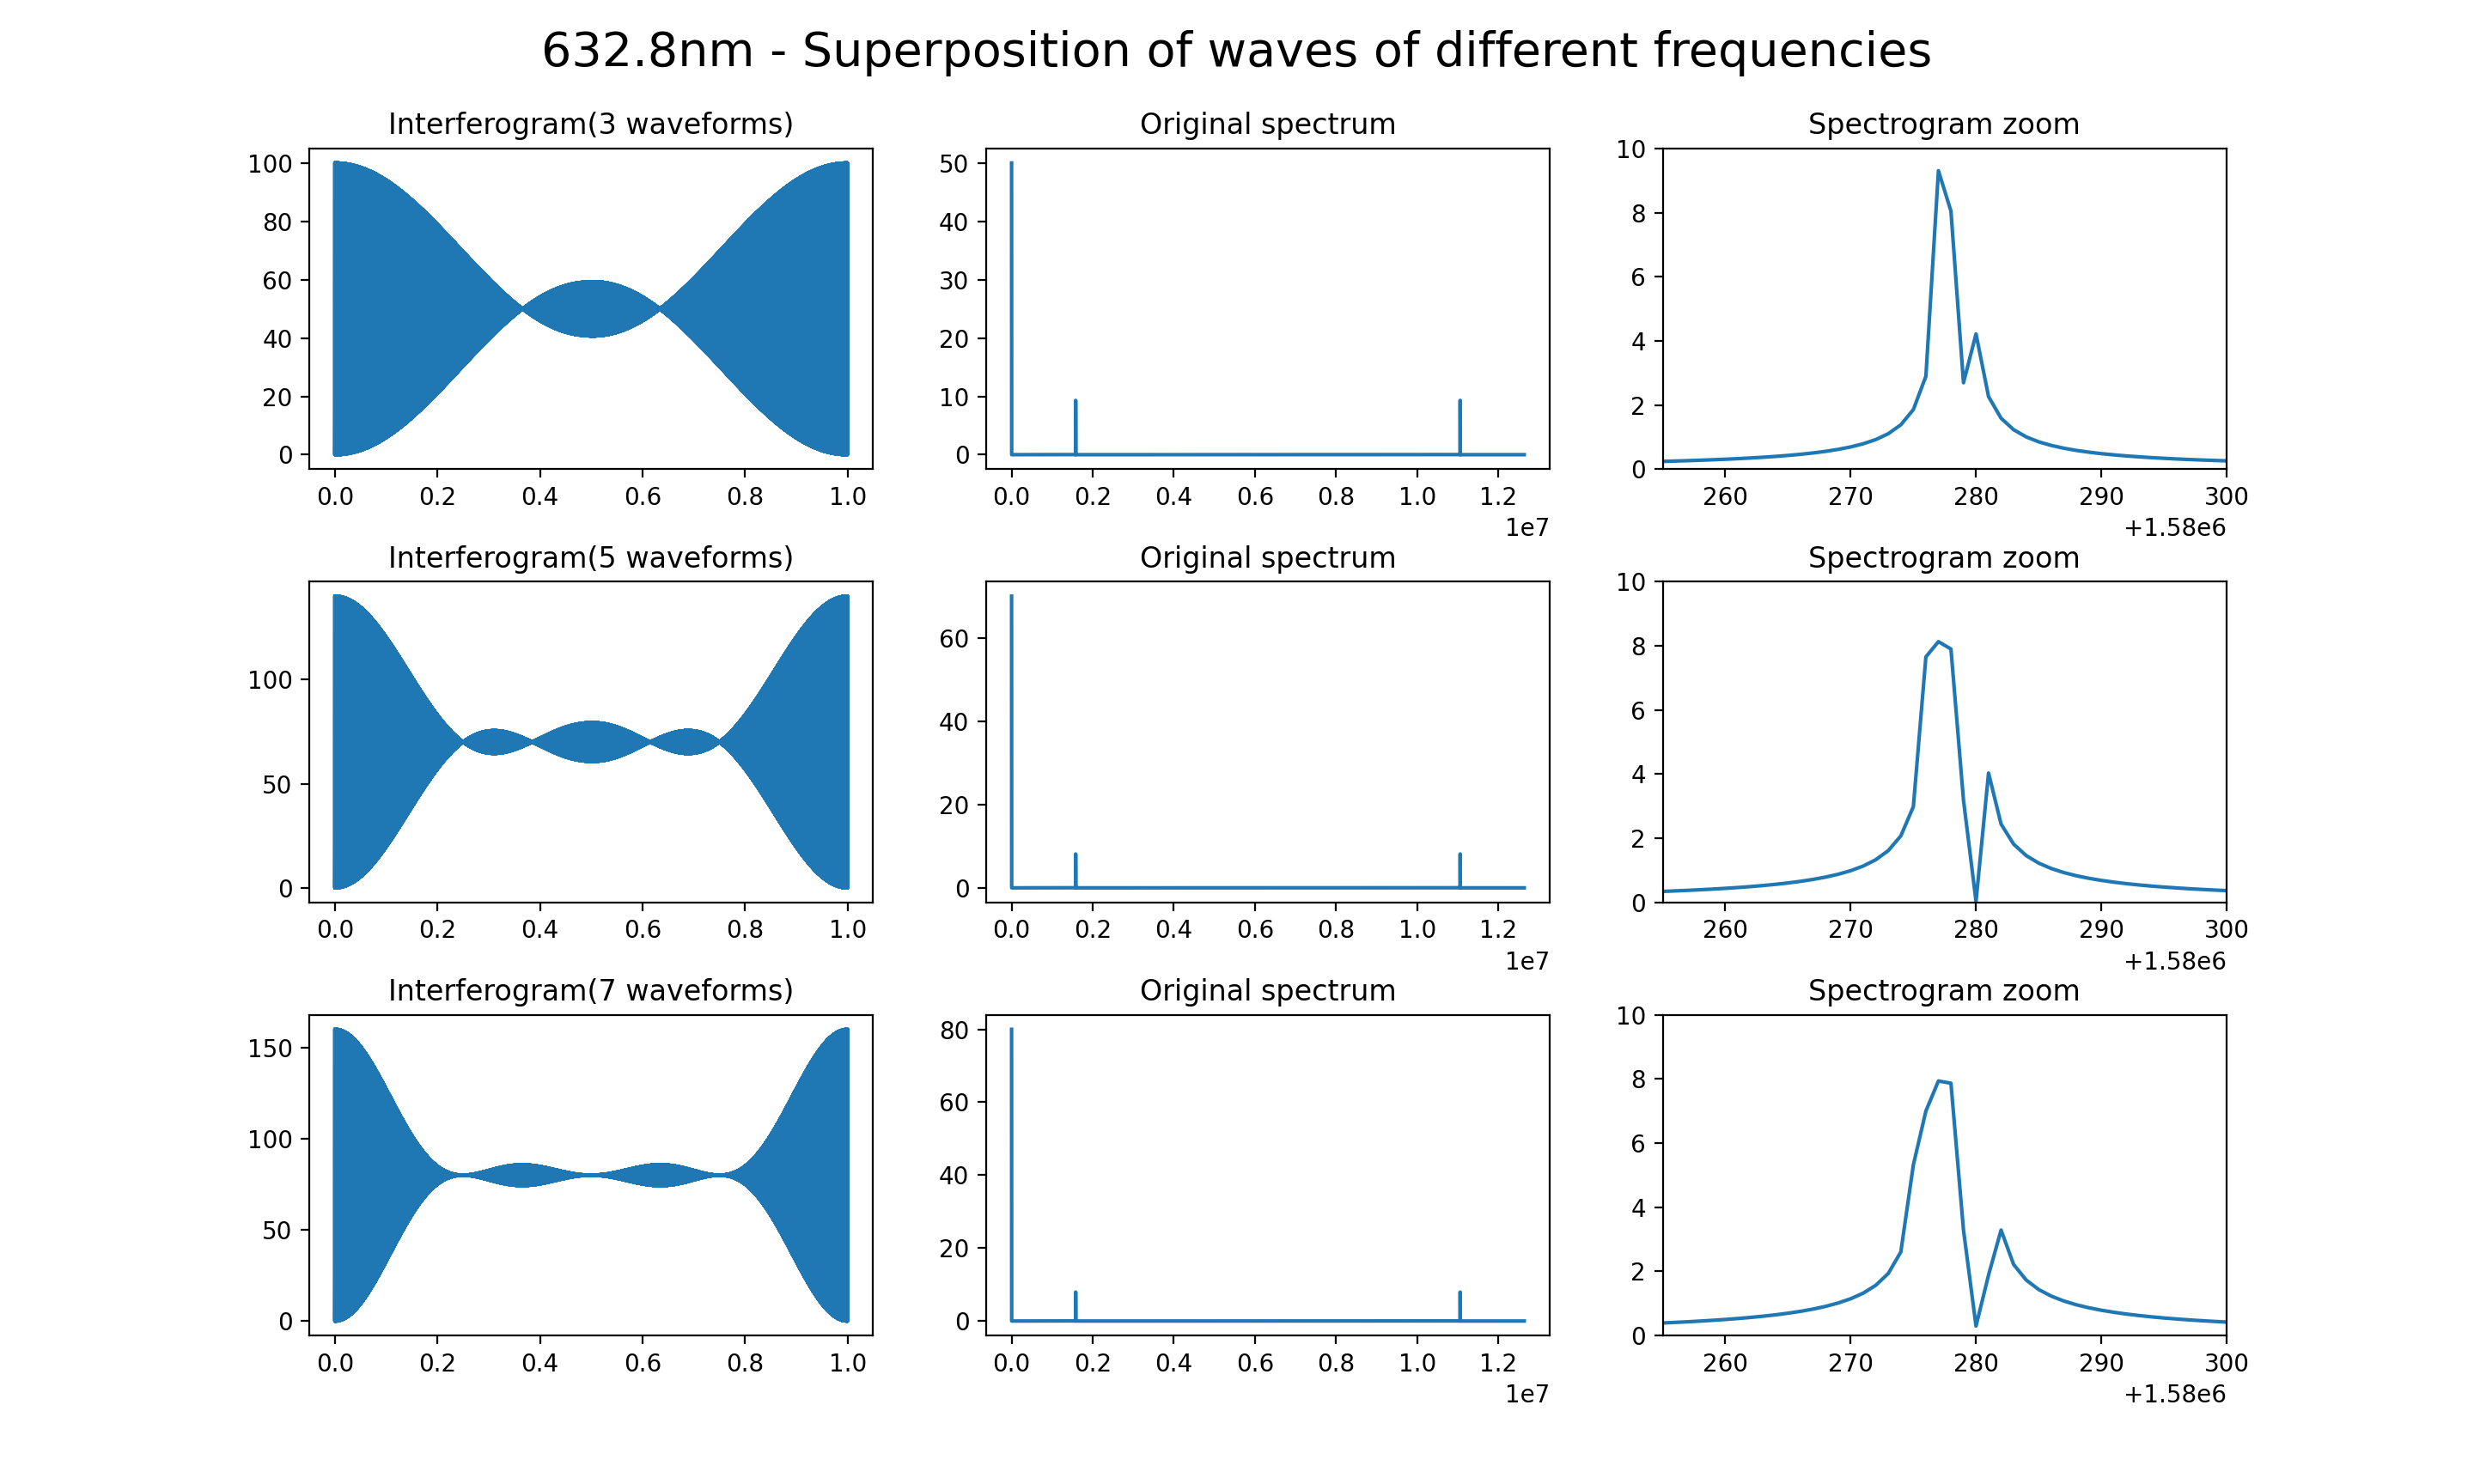
\includegraphics[width=0.5\textwidth]{pic17.png}}
    \caption{非单纵模 (多频) 激光输入FTS(情况8)}
    \label{pic17}
\end{figure}

图\ref{pic18}显示了奇数个干涉强度相同的波的叠加干涉图,具体参数为
\begin{itemize}
    \item 叠加波的频率不同
    \item 幅值相同
    \item 扫描长度:2m
    \item 中心波长:632.8nm
    \item 采样间隔:632.8nm/4
    \item 频率间隔:300MHz
\end{itemize}
\begin{figure}[htbp]
    \centerline{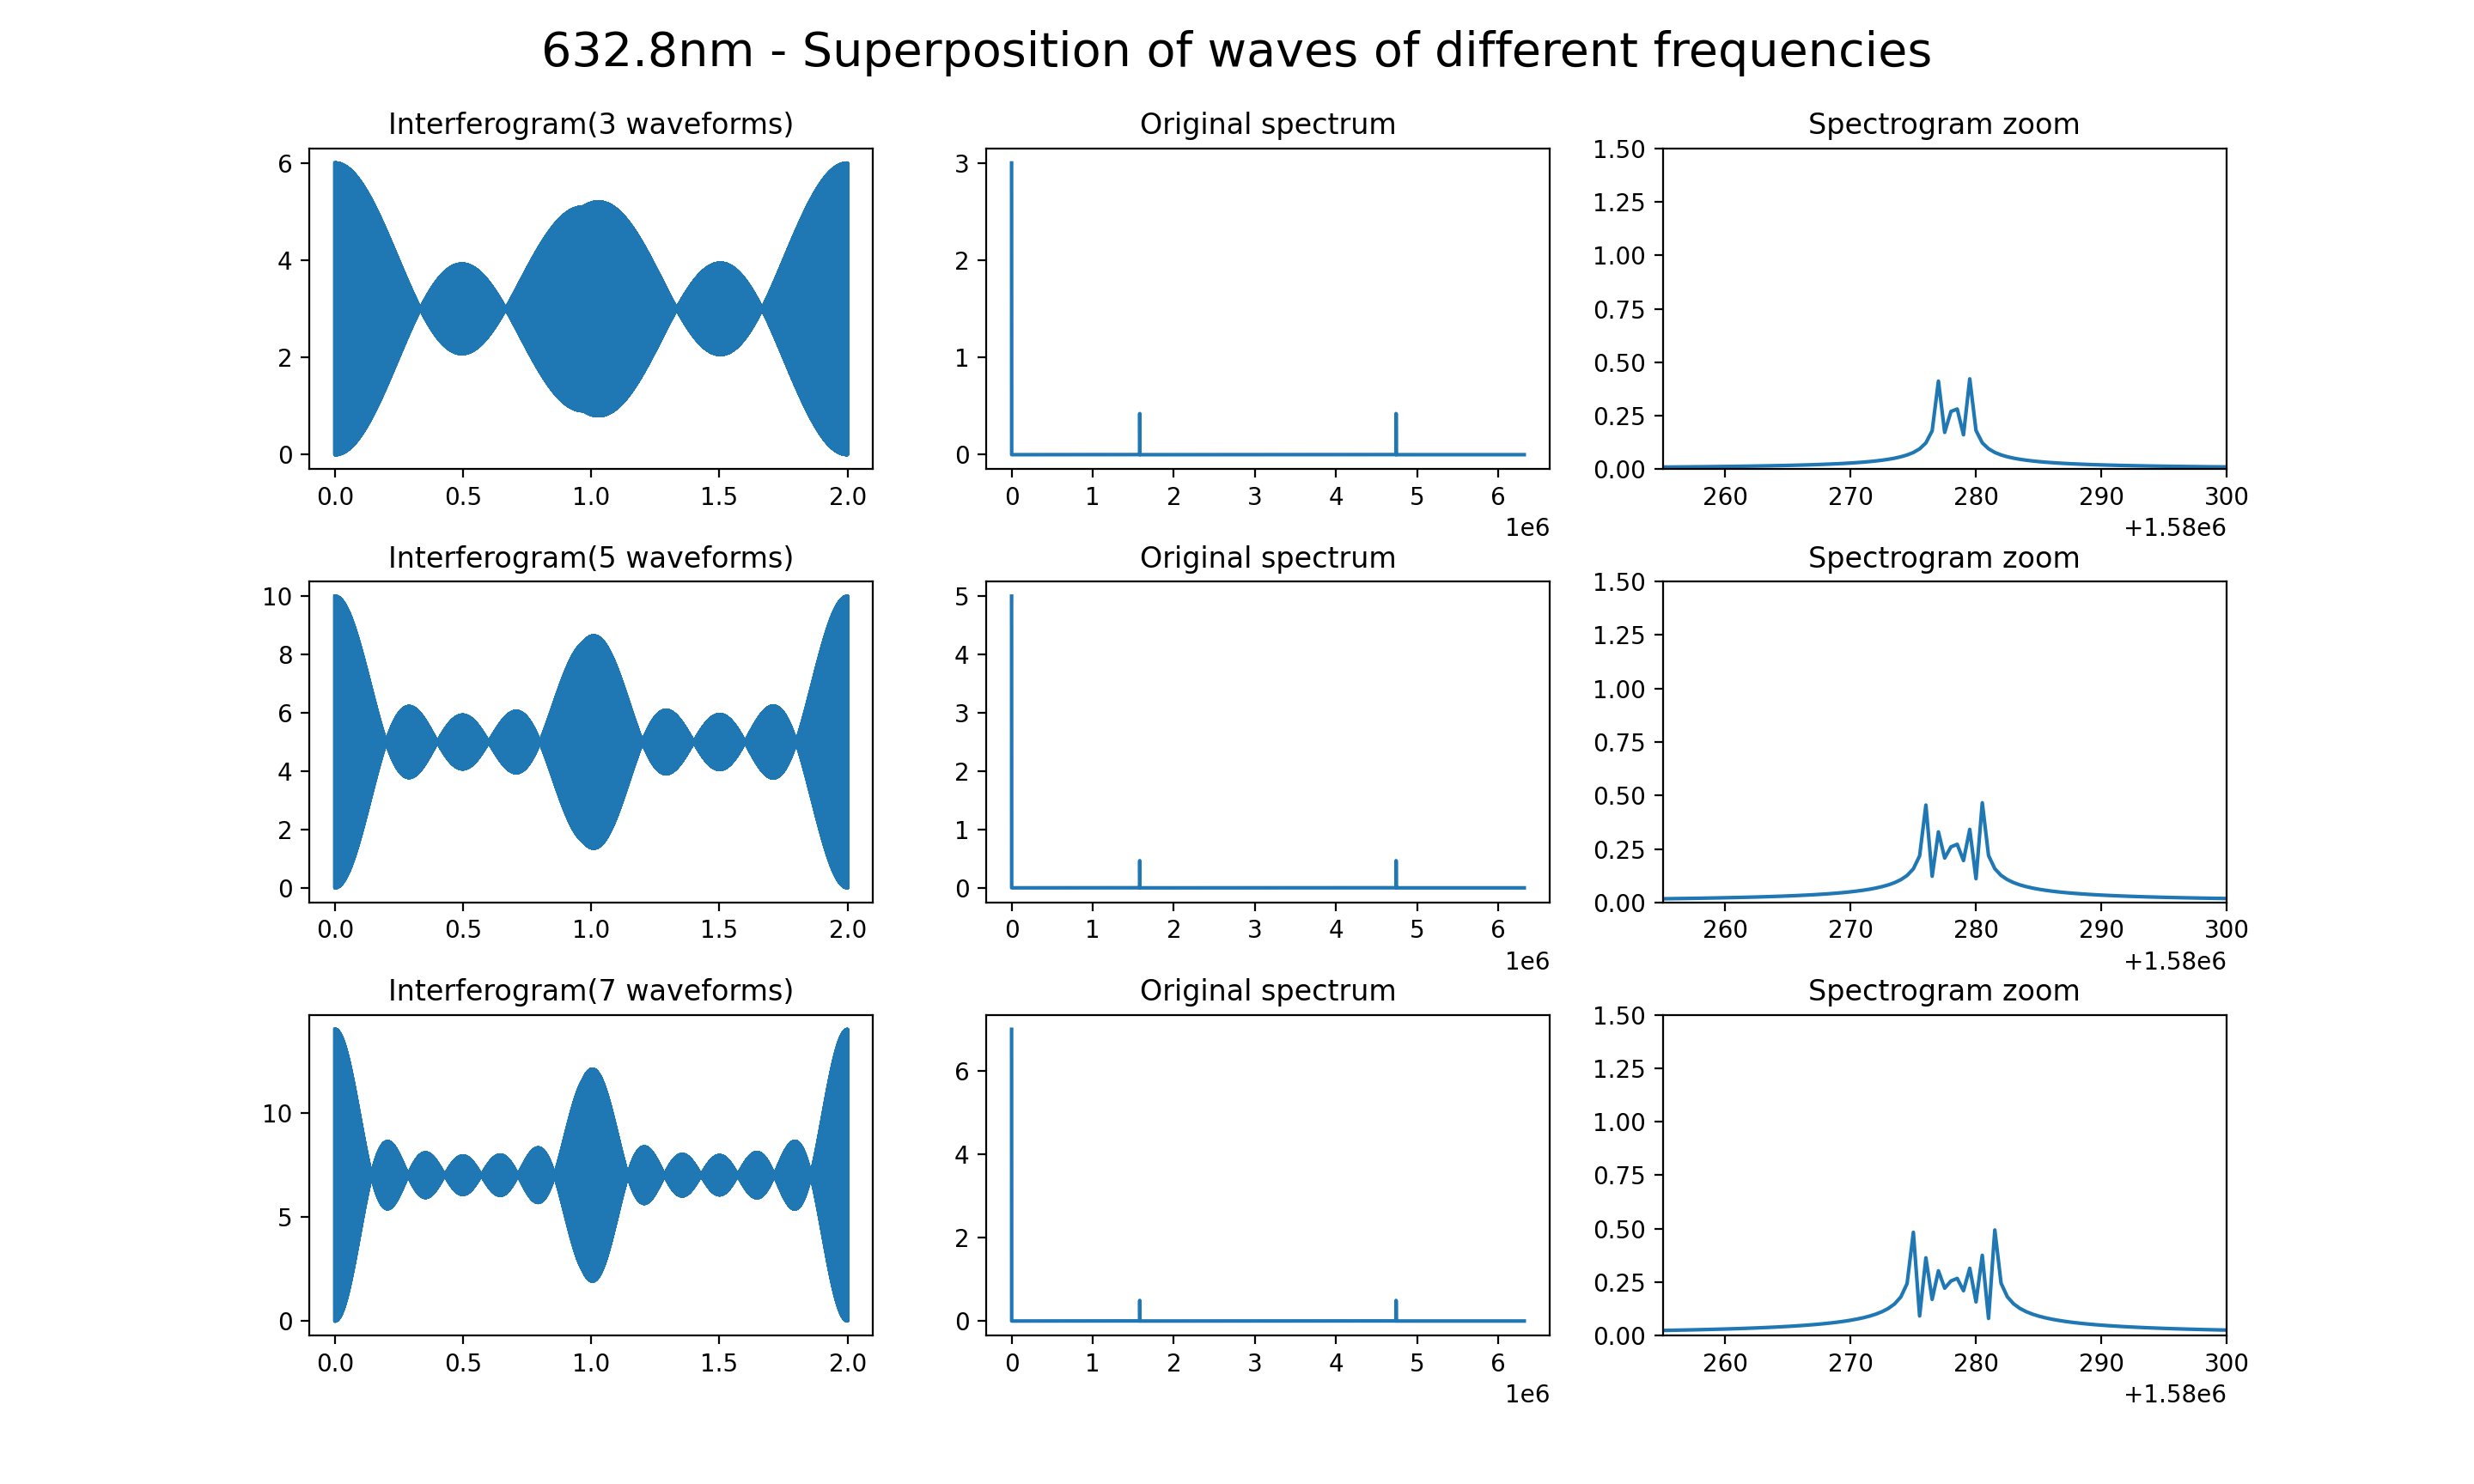
\includegraphics[width=0.5\textwidth]{pic18.png}}
    \caption{非单纵模 (多频) 激光输入FTS(情况9)}
    \label{pic18}
\end{figure}

图\ref{pic19}显示了奇数个干涉强度相同的波的叠加干涉图,具体参数为
\begin{itemize}
    \item 叠加波的频率不同
    \item 幅值相同
    \item 扫描长度:2m
    \item 中心波长:632.8nm
    \item 采样间隔:632.8nm/8
    \item 频率间隔:300MHz
\end{itemize}
\begin{figure}[htbp]
    \centerline{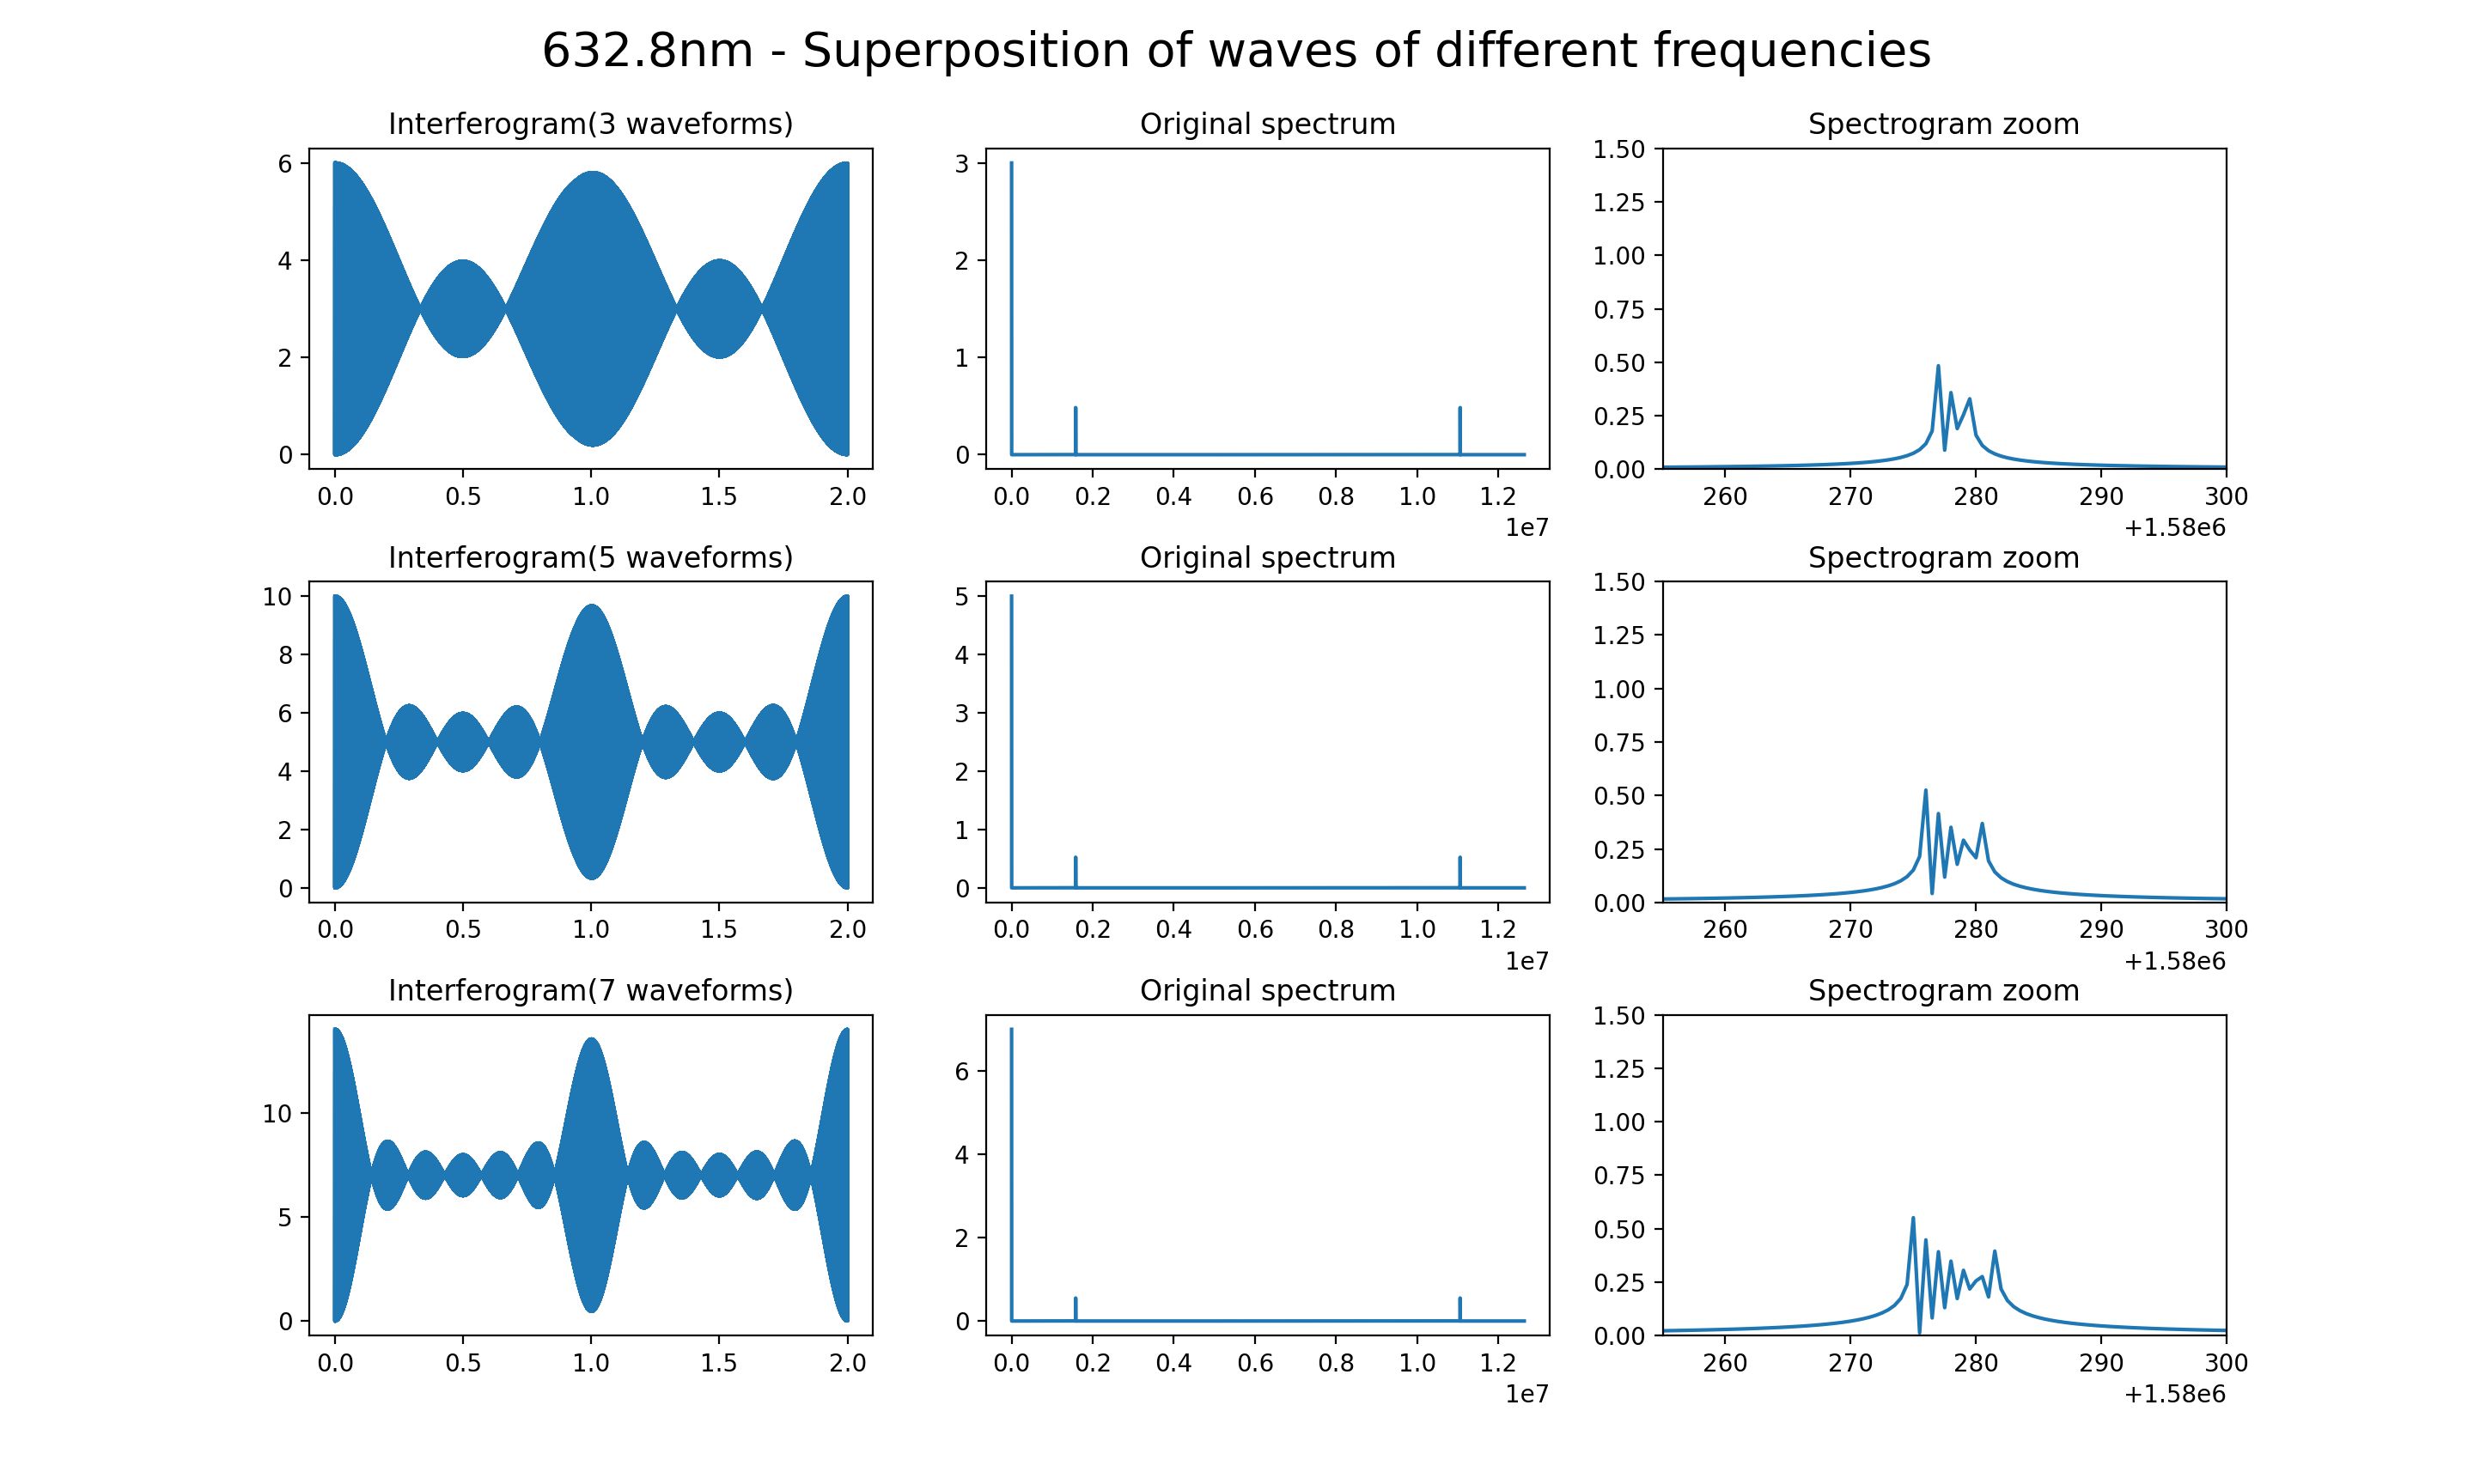
\includegraphics[width=0.5\textwidth]{pic19.png}}
    \caption{非单纵模 (多频) 激光输入FTS(情况10)}
    \label{pic19}
\end{figure}

图\ref{pic20}显示了奇数个干涉强度相同的波的叠加干涉图,具体参数为
\begin{itemize}
    \item 叠加波的频率不同
    \item 幅值相同
    \item 扫描长度:2m
    \item 中心波长:532nm
    \item 采样间隔:632.8nm/4
    \item 频率间隔:300MHz
\end{itemize}
\begin{figure}[htbp]
    \centerline{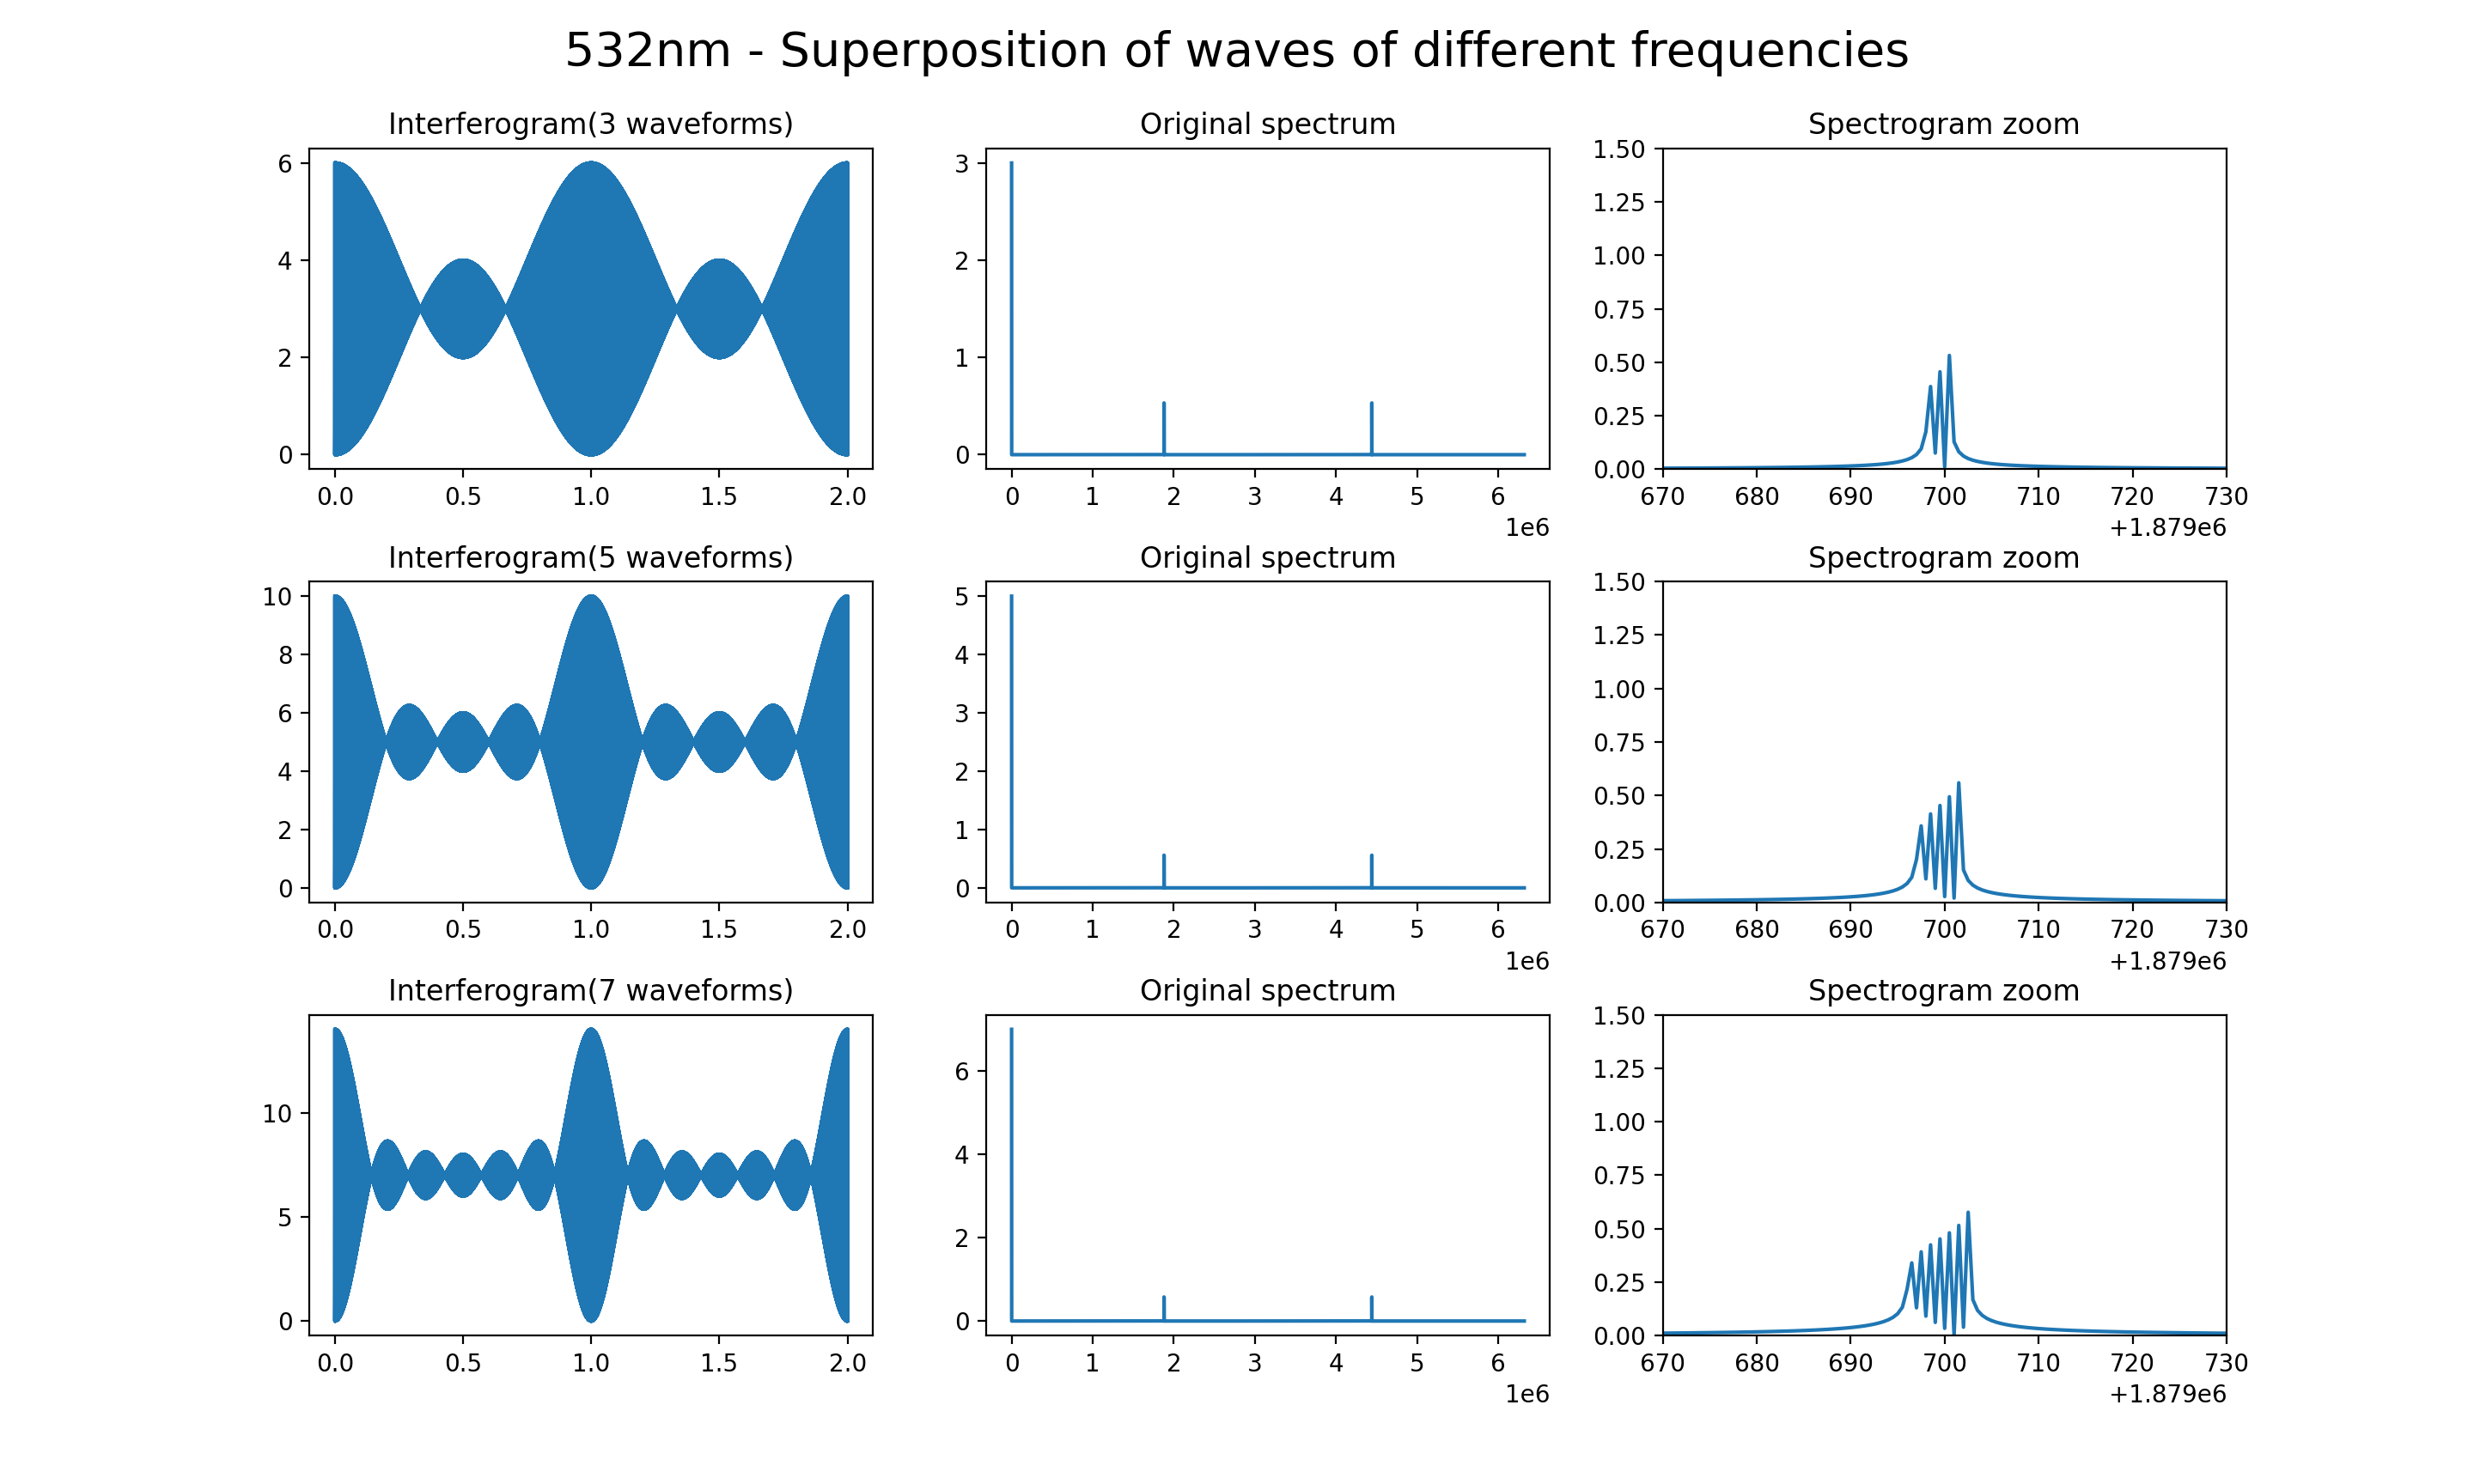
\includegraphics[width=0.5\textwidth]{pic20.png}}
    \caption{非单纵模 (多频) 激光输入FTS(情况11)}
    \label{pic20}
\end{figure}

图\ref{pic21}显示了奇数个干涉强度相同的波的叠加干涉图,具体参数为
\begin{itemize}
    \item 叠加波的频率不同
    \item 幅值相同
    \item 扫描长度:2m
    \item 中心波长:532nm
    \item 采样间隔:632.8nm/8
    \item 频率间隔:300MHz
\end{itemize}
\begin{figure}[htbp]
    \centerline{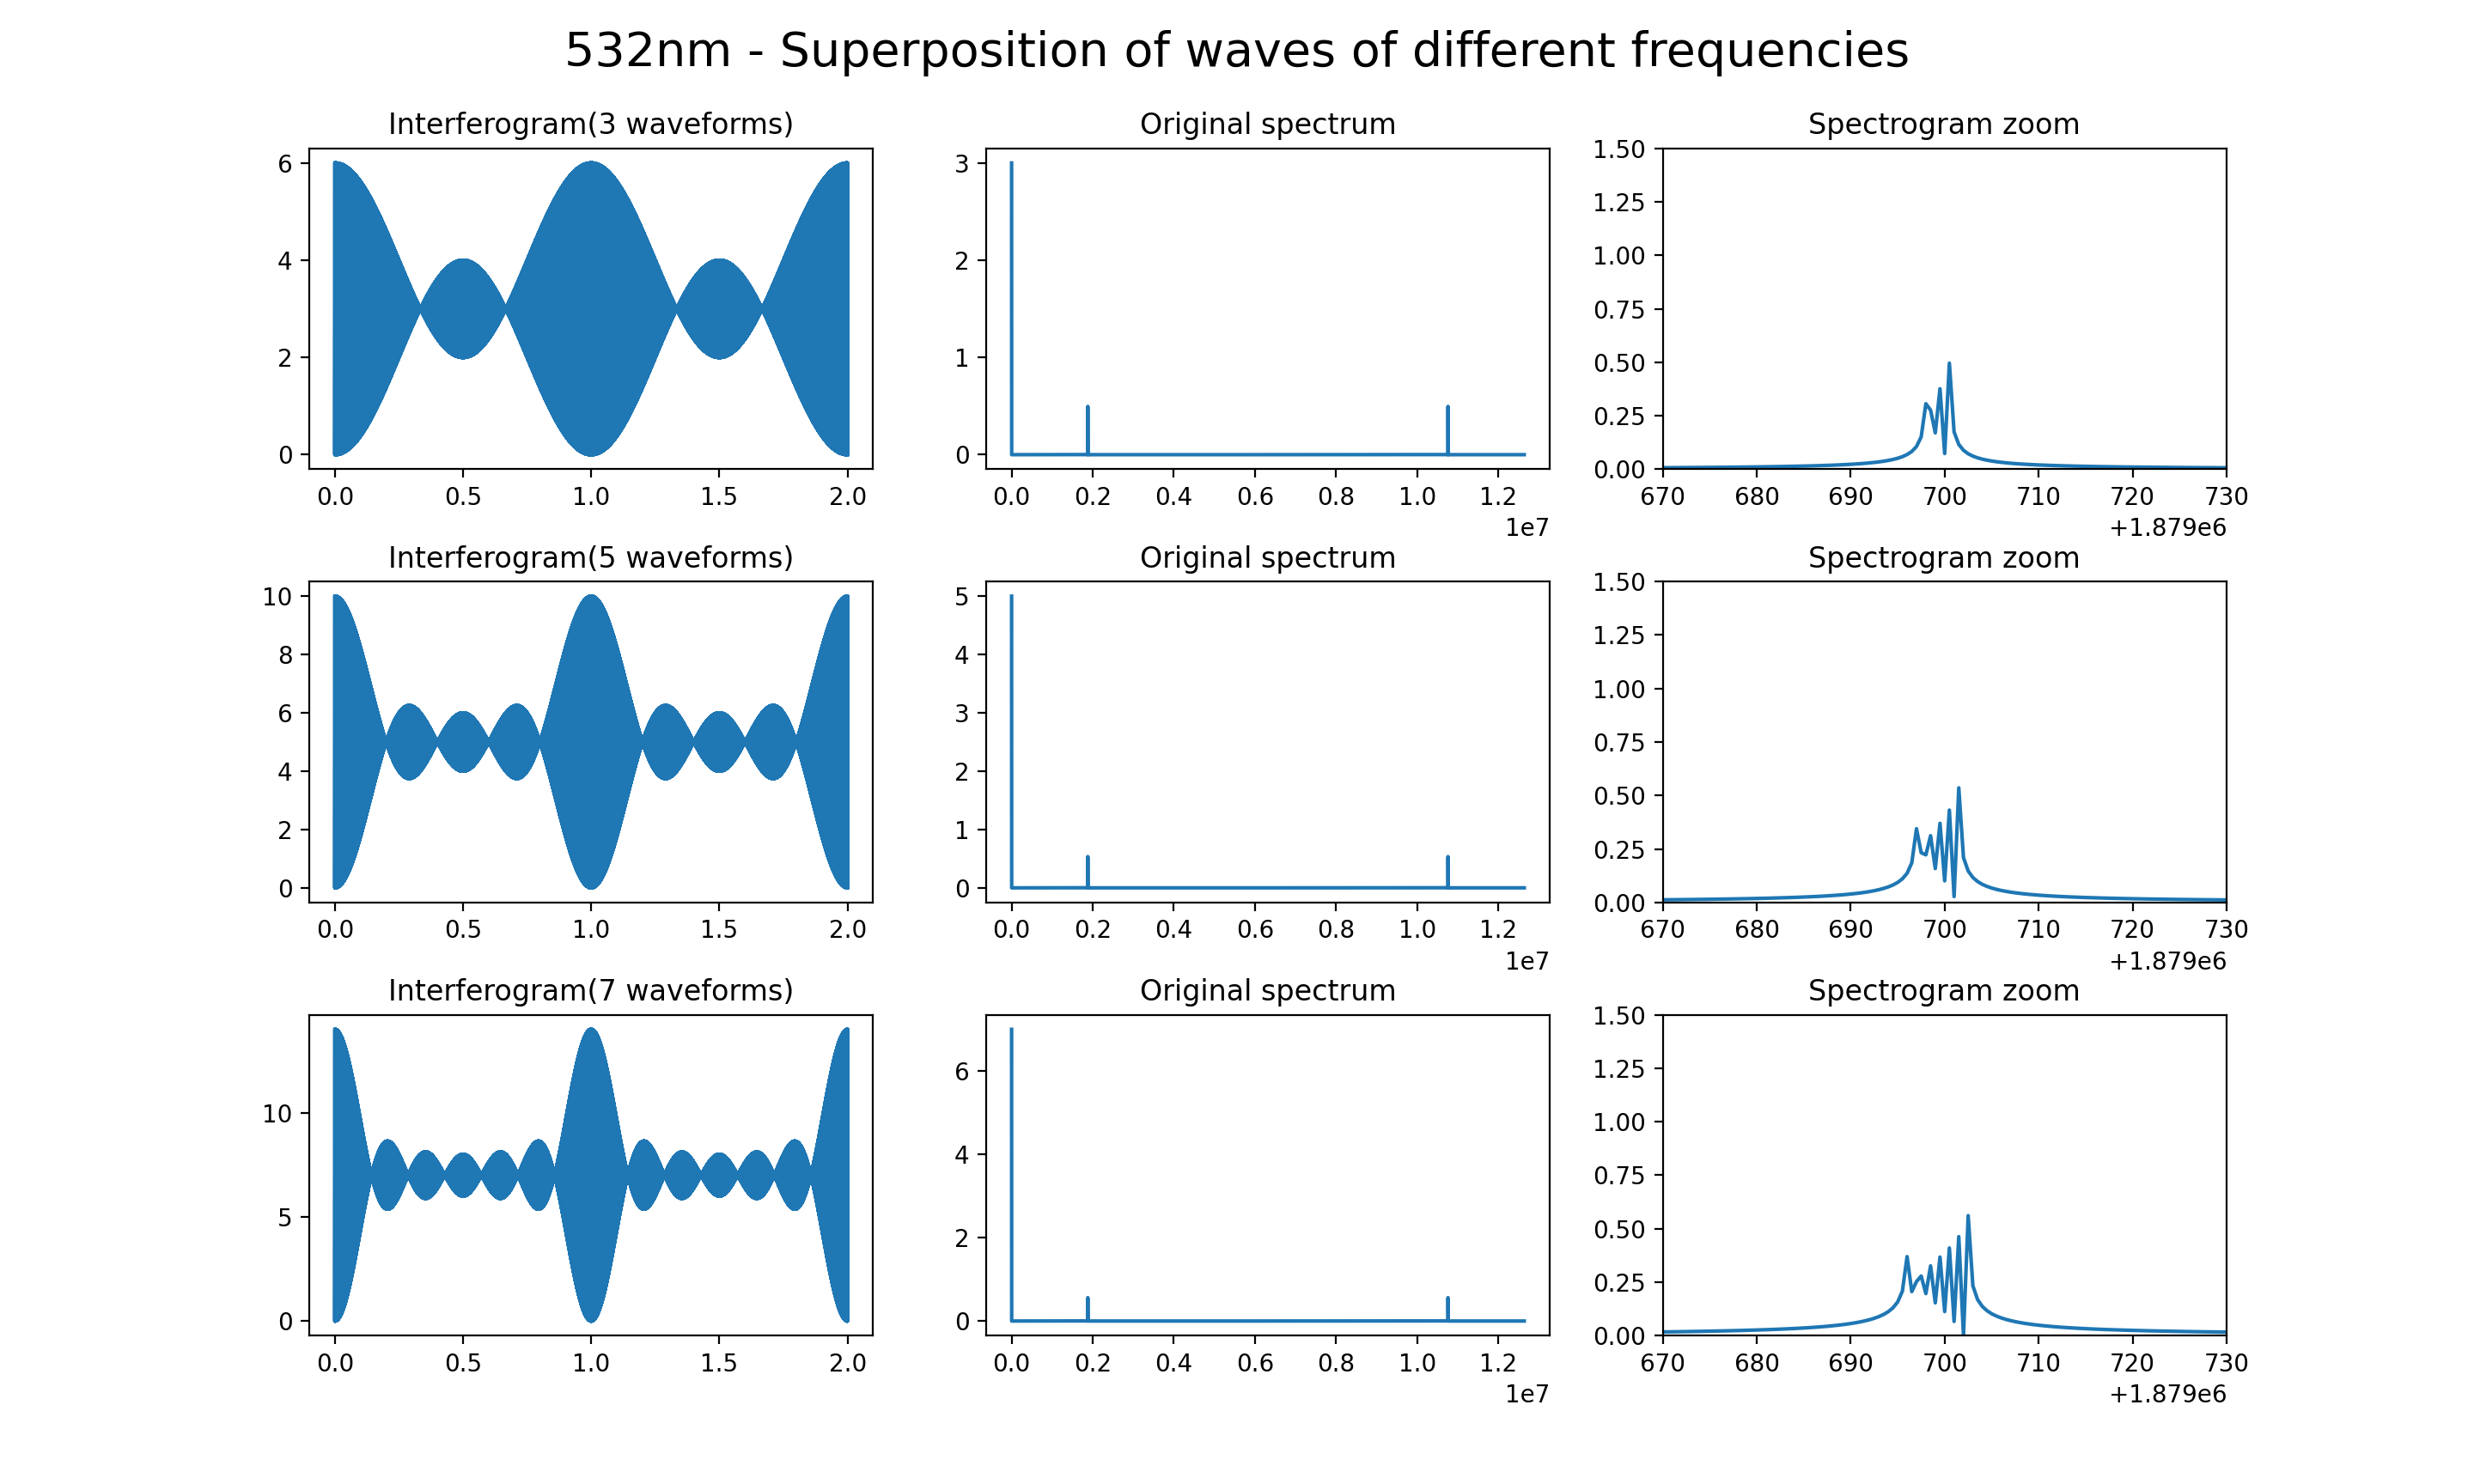
\includegraphics[width=0.6\textwidth]{pic21.png}}
    \caption{非单纵模 (多频) 激光输入FTS(情况12)}
    \label{pic21}
\end{figure}

图\ref{pic22}显示了奇数个干涉强度相同的波的叠加干涉图,具体参数为
\begin{itemize}
    \item 叠加波的频率不同
    \item 幅值不相同
    \item 扫描长度:2m
    \item 中心波长:632.8nm
    \item 采样间隔:632.8nm/4
    \item 频率间隔:300MHz
\end{itemize}
\begin{figure}[htbp]
    \centerline{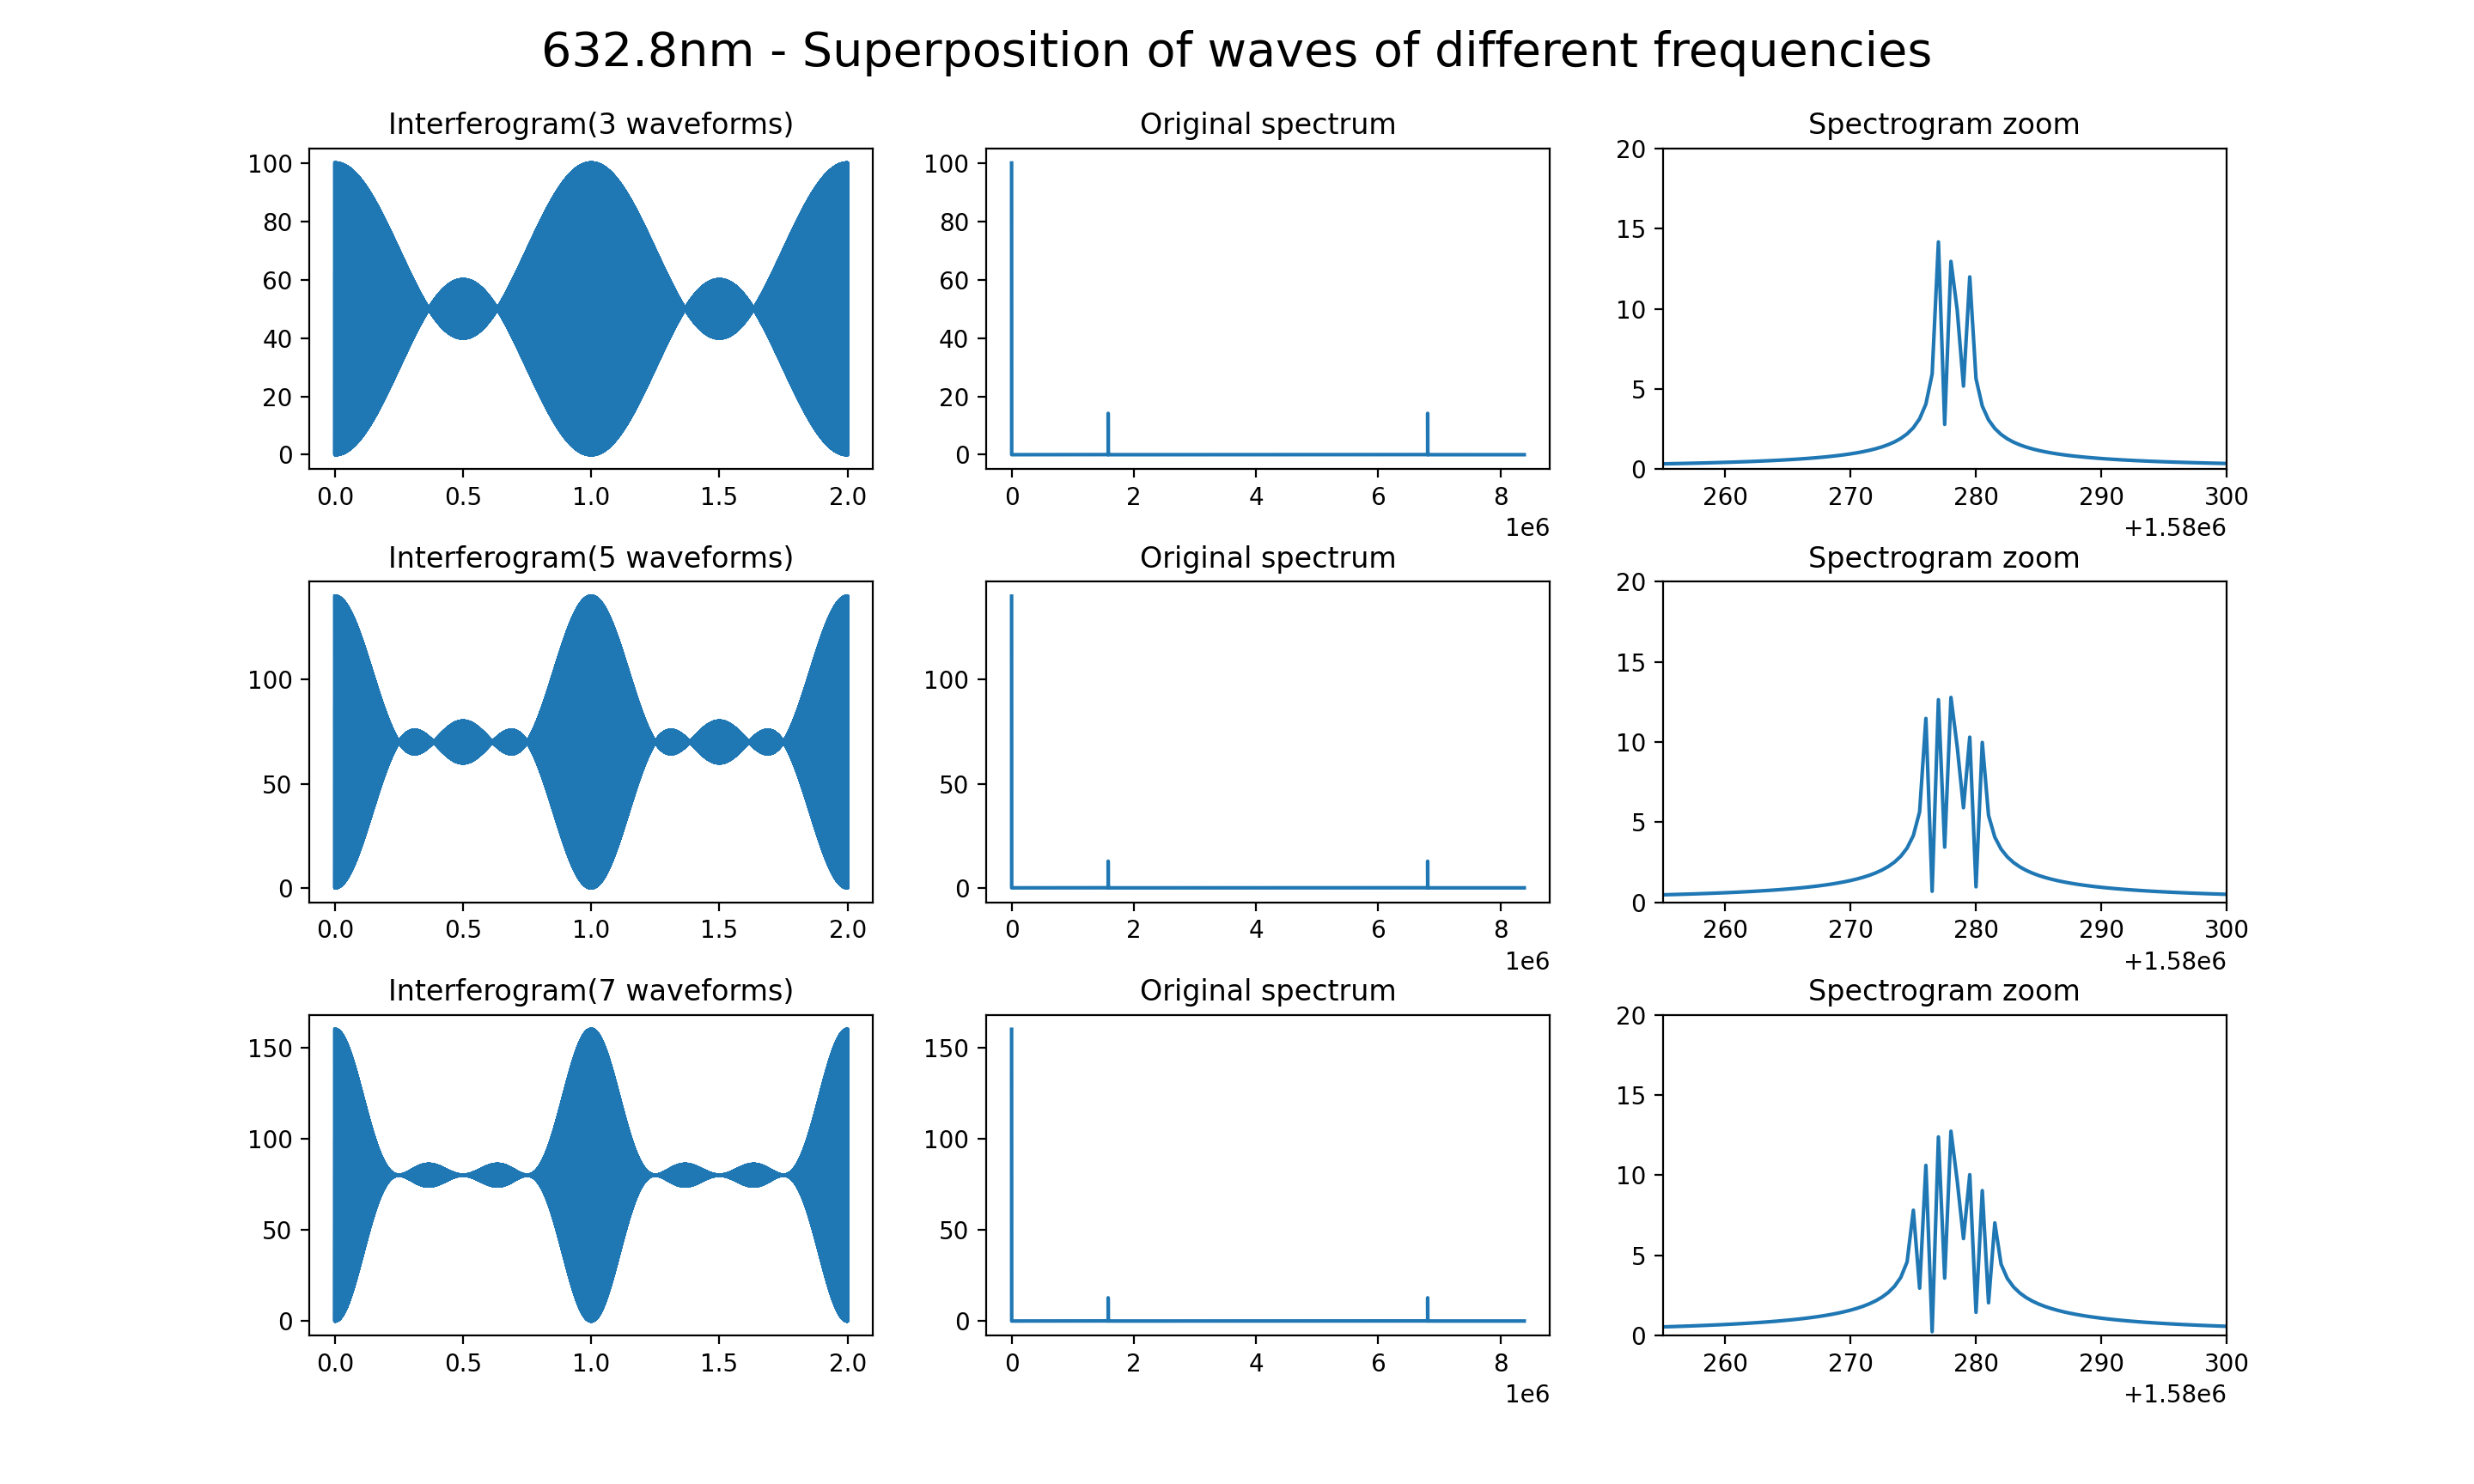
\includegraphics[width=0.5\textwidth]{pic22.png}}
    \caption{非单纵模 (多频) 激光输入FTS(情况13)}
    \label{pic22}
\end{figure}

图\ref{pic23}显示了奇数个干涉强度相同的波的叠加干涉图,具体参数为
\begin{itemize}
    \item 叠加波的频率不同
    \item 幅值不相同
    \item 扫描长度:2m
    \item 中心波长:632.8nm
    \item 采样间隔:632.8nm/8
    \item 频率间隔:300MHz
\end{itemize}
\begin{figure}[htbp]
    \centerline{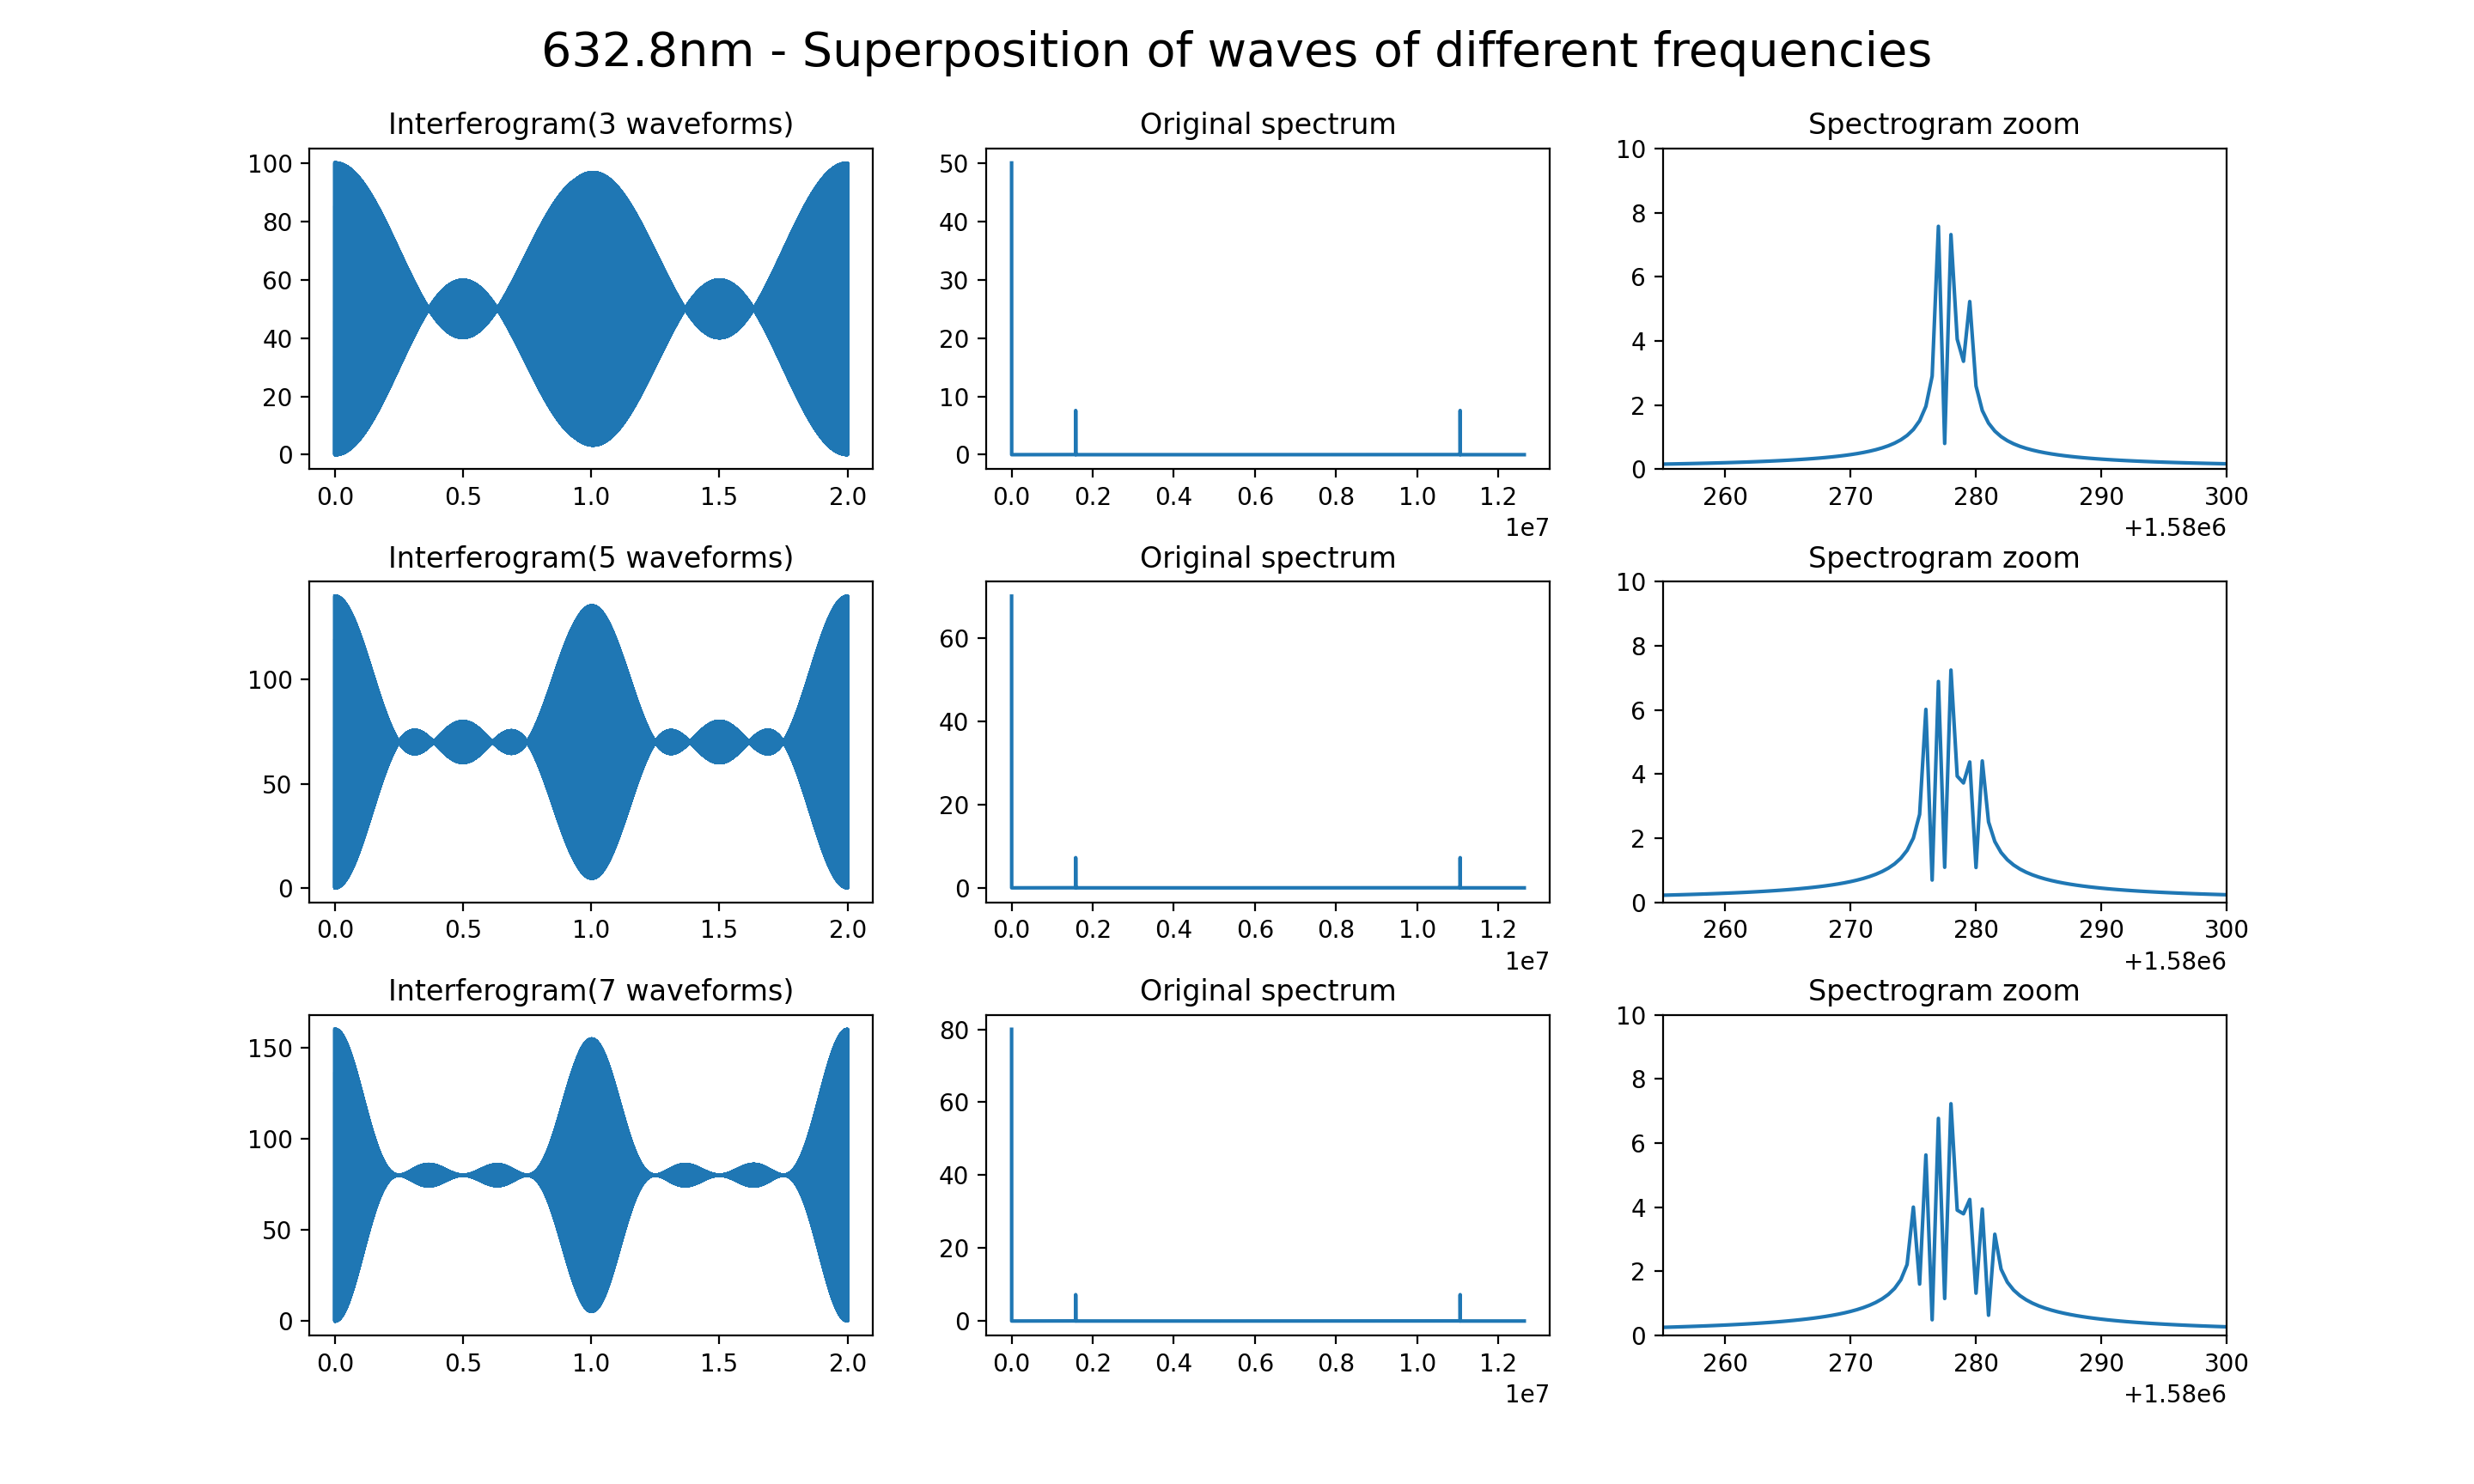
\includegraphics[width=0.5\textwidth]{pic23.png}}
    \caption{非单纵模 (多频) 激光输入FTS(情况14)}
    \label{pic23}
\end{figure}

图\ref{pic24}显示了奇数个干涉强度相同的波的叠加干涉图,具体参数为
\begin{itemize}
    \item 叠加波的频率不同
    \item 幅值不相同
    \item 扫描长度:2m
    \item 中心波长:532nm
    \item 采样间隔:632.8nm/4
    \item 频率间隔:300MHz
\end{itemize}
\begin{figure}[htbp]
    \centerline{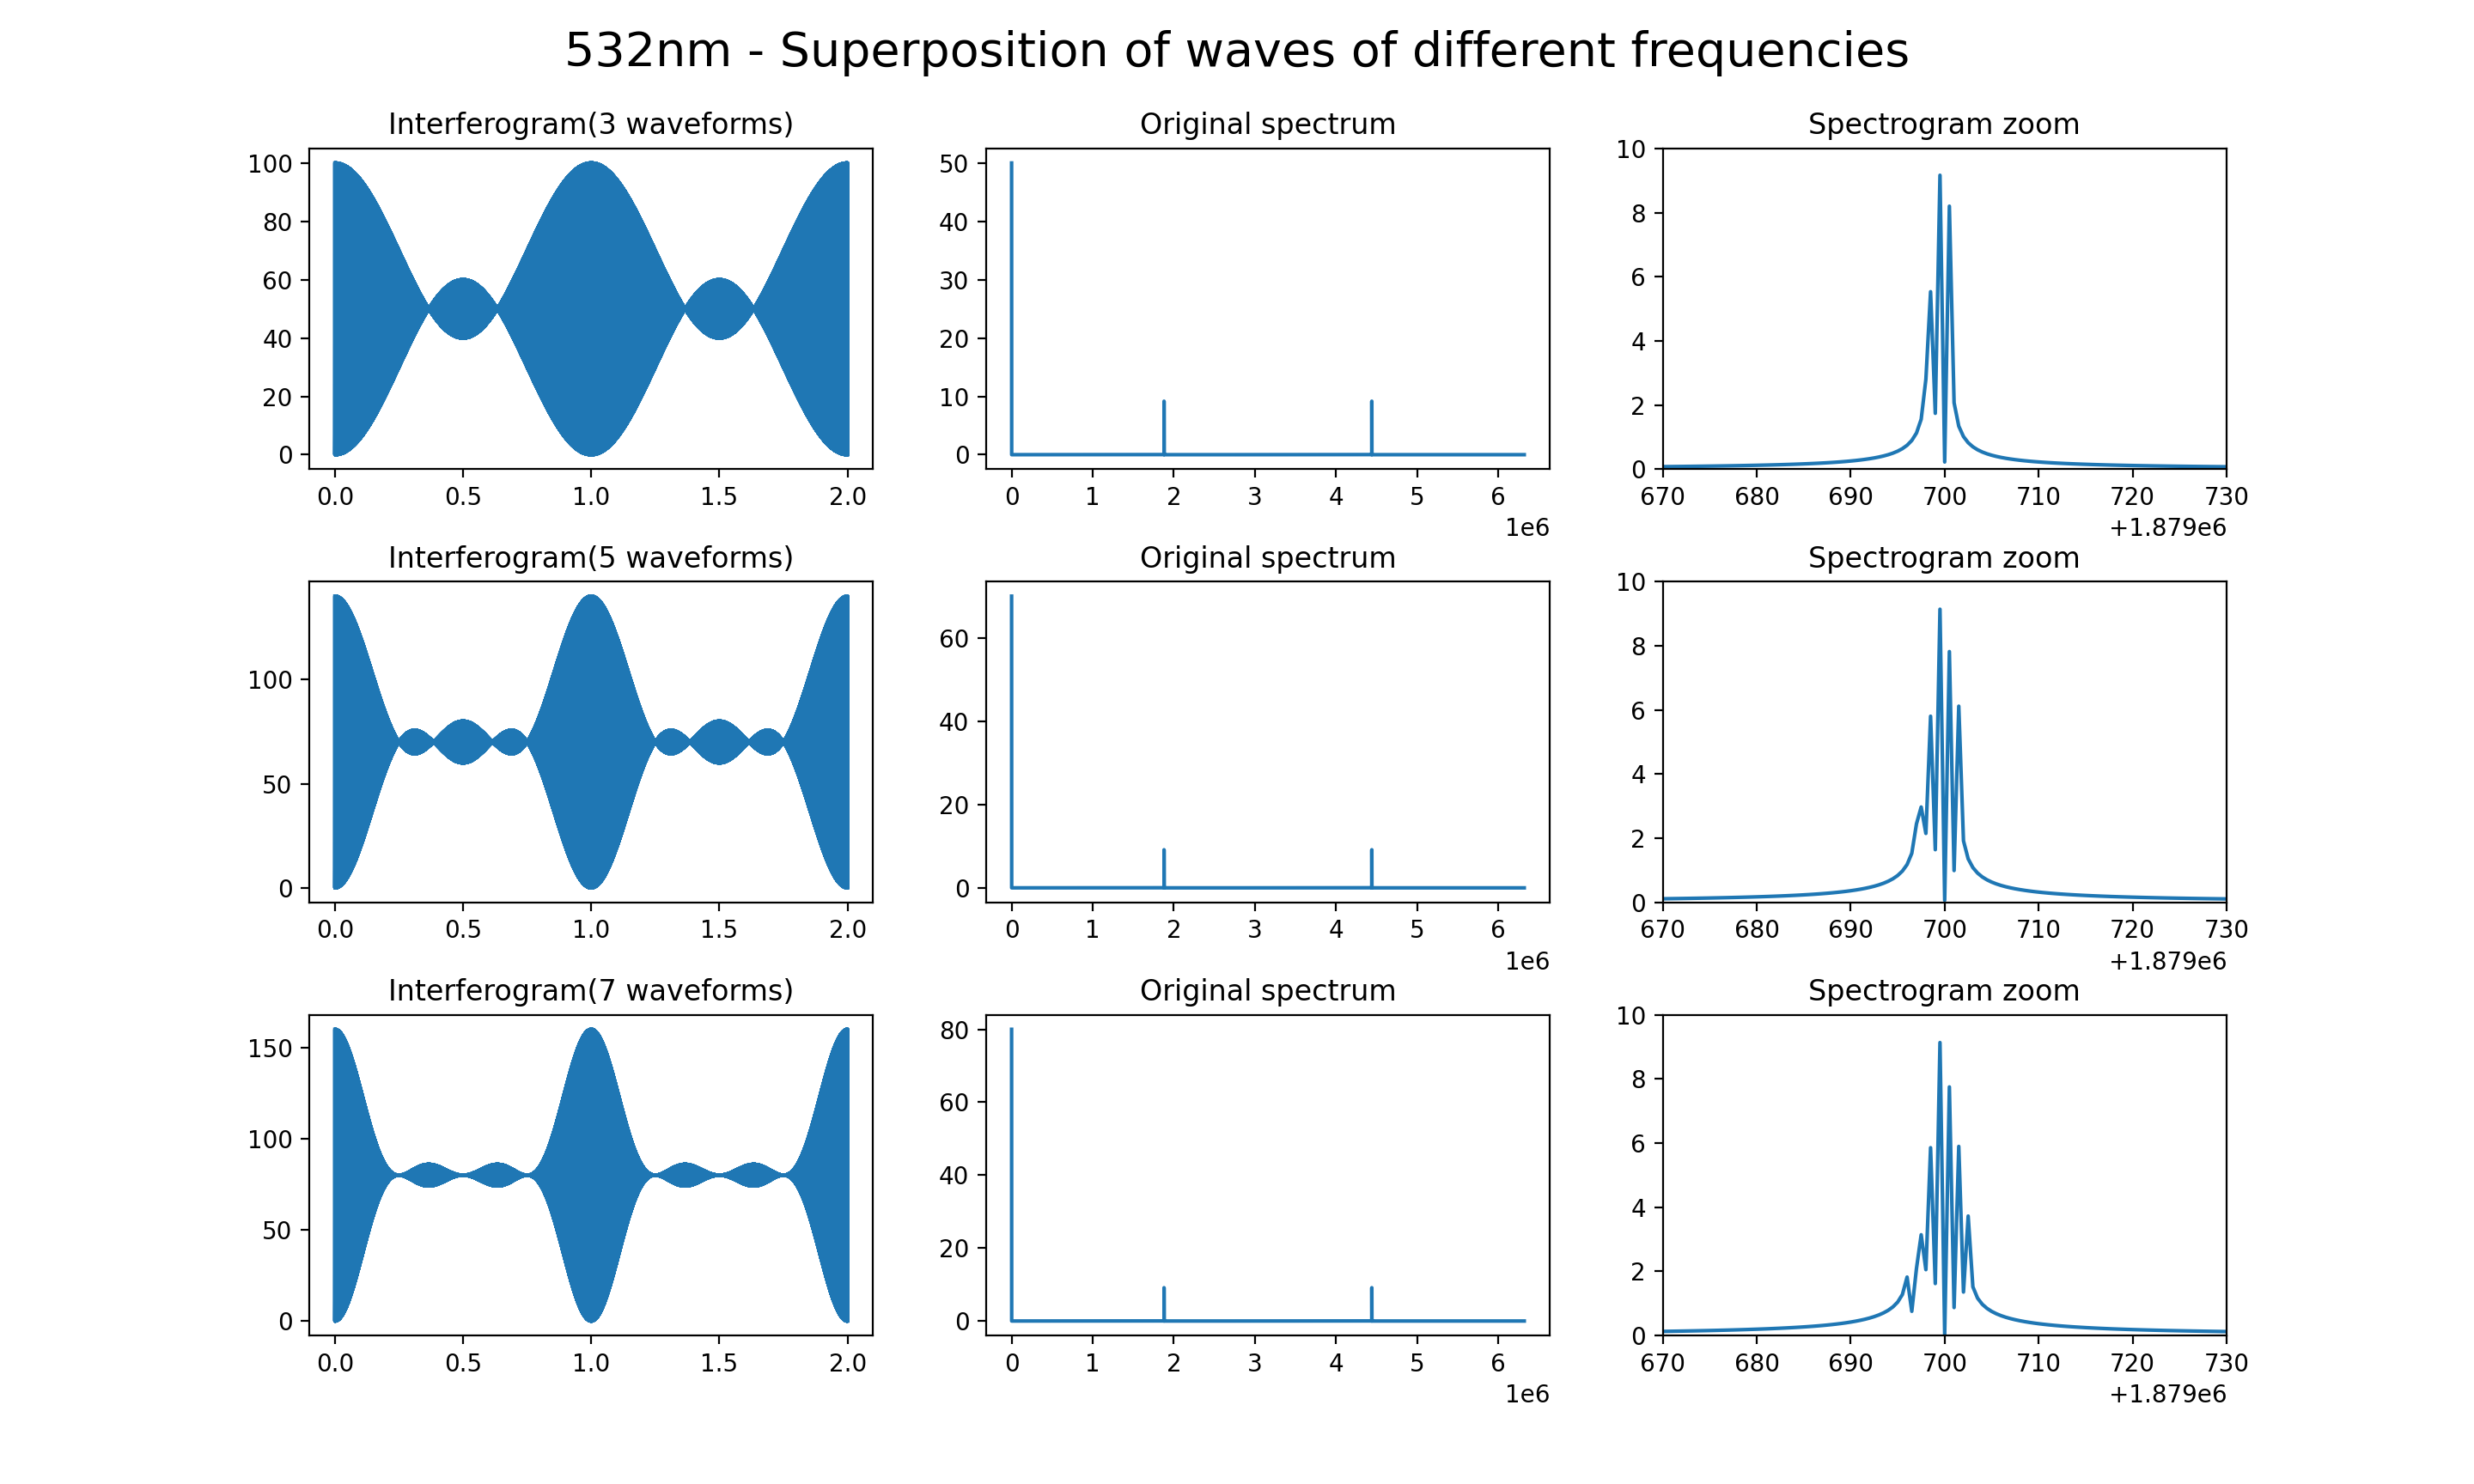
\includegraphics[width=0.5\textwidth]{pic24.png}}
    \caption{非单纵模 (多频) 激光输入FTS(情况15)}
    \label{pic24}
\end{figure}

图\ref{pic25}显示了奇数个干涉强度相同的波的叠加干涉图,具体参数为
\begin{itemize}
    \item 叠加波的频率不同
    \item 幅值不相同
    \item 扫描长度:2m
    \item 中心波长:532nm
    \item 采样间隔:632.8nm/8
    \item 频率间隔:300MHz
\end{itemize}
\begin{figure}[htbp]
    \centerline{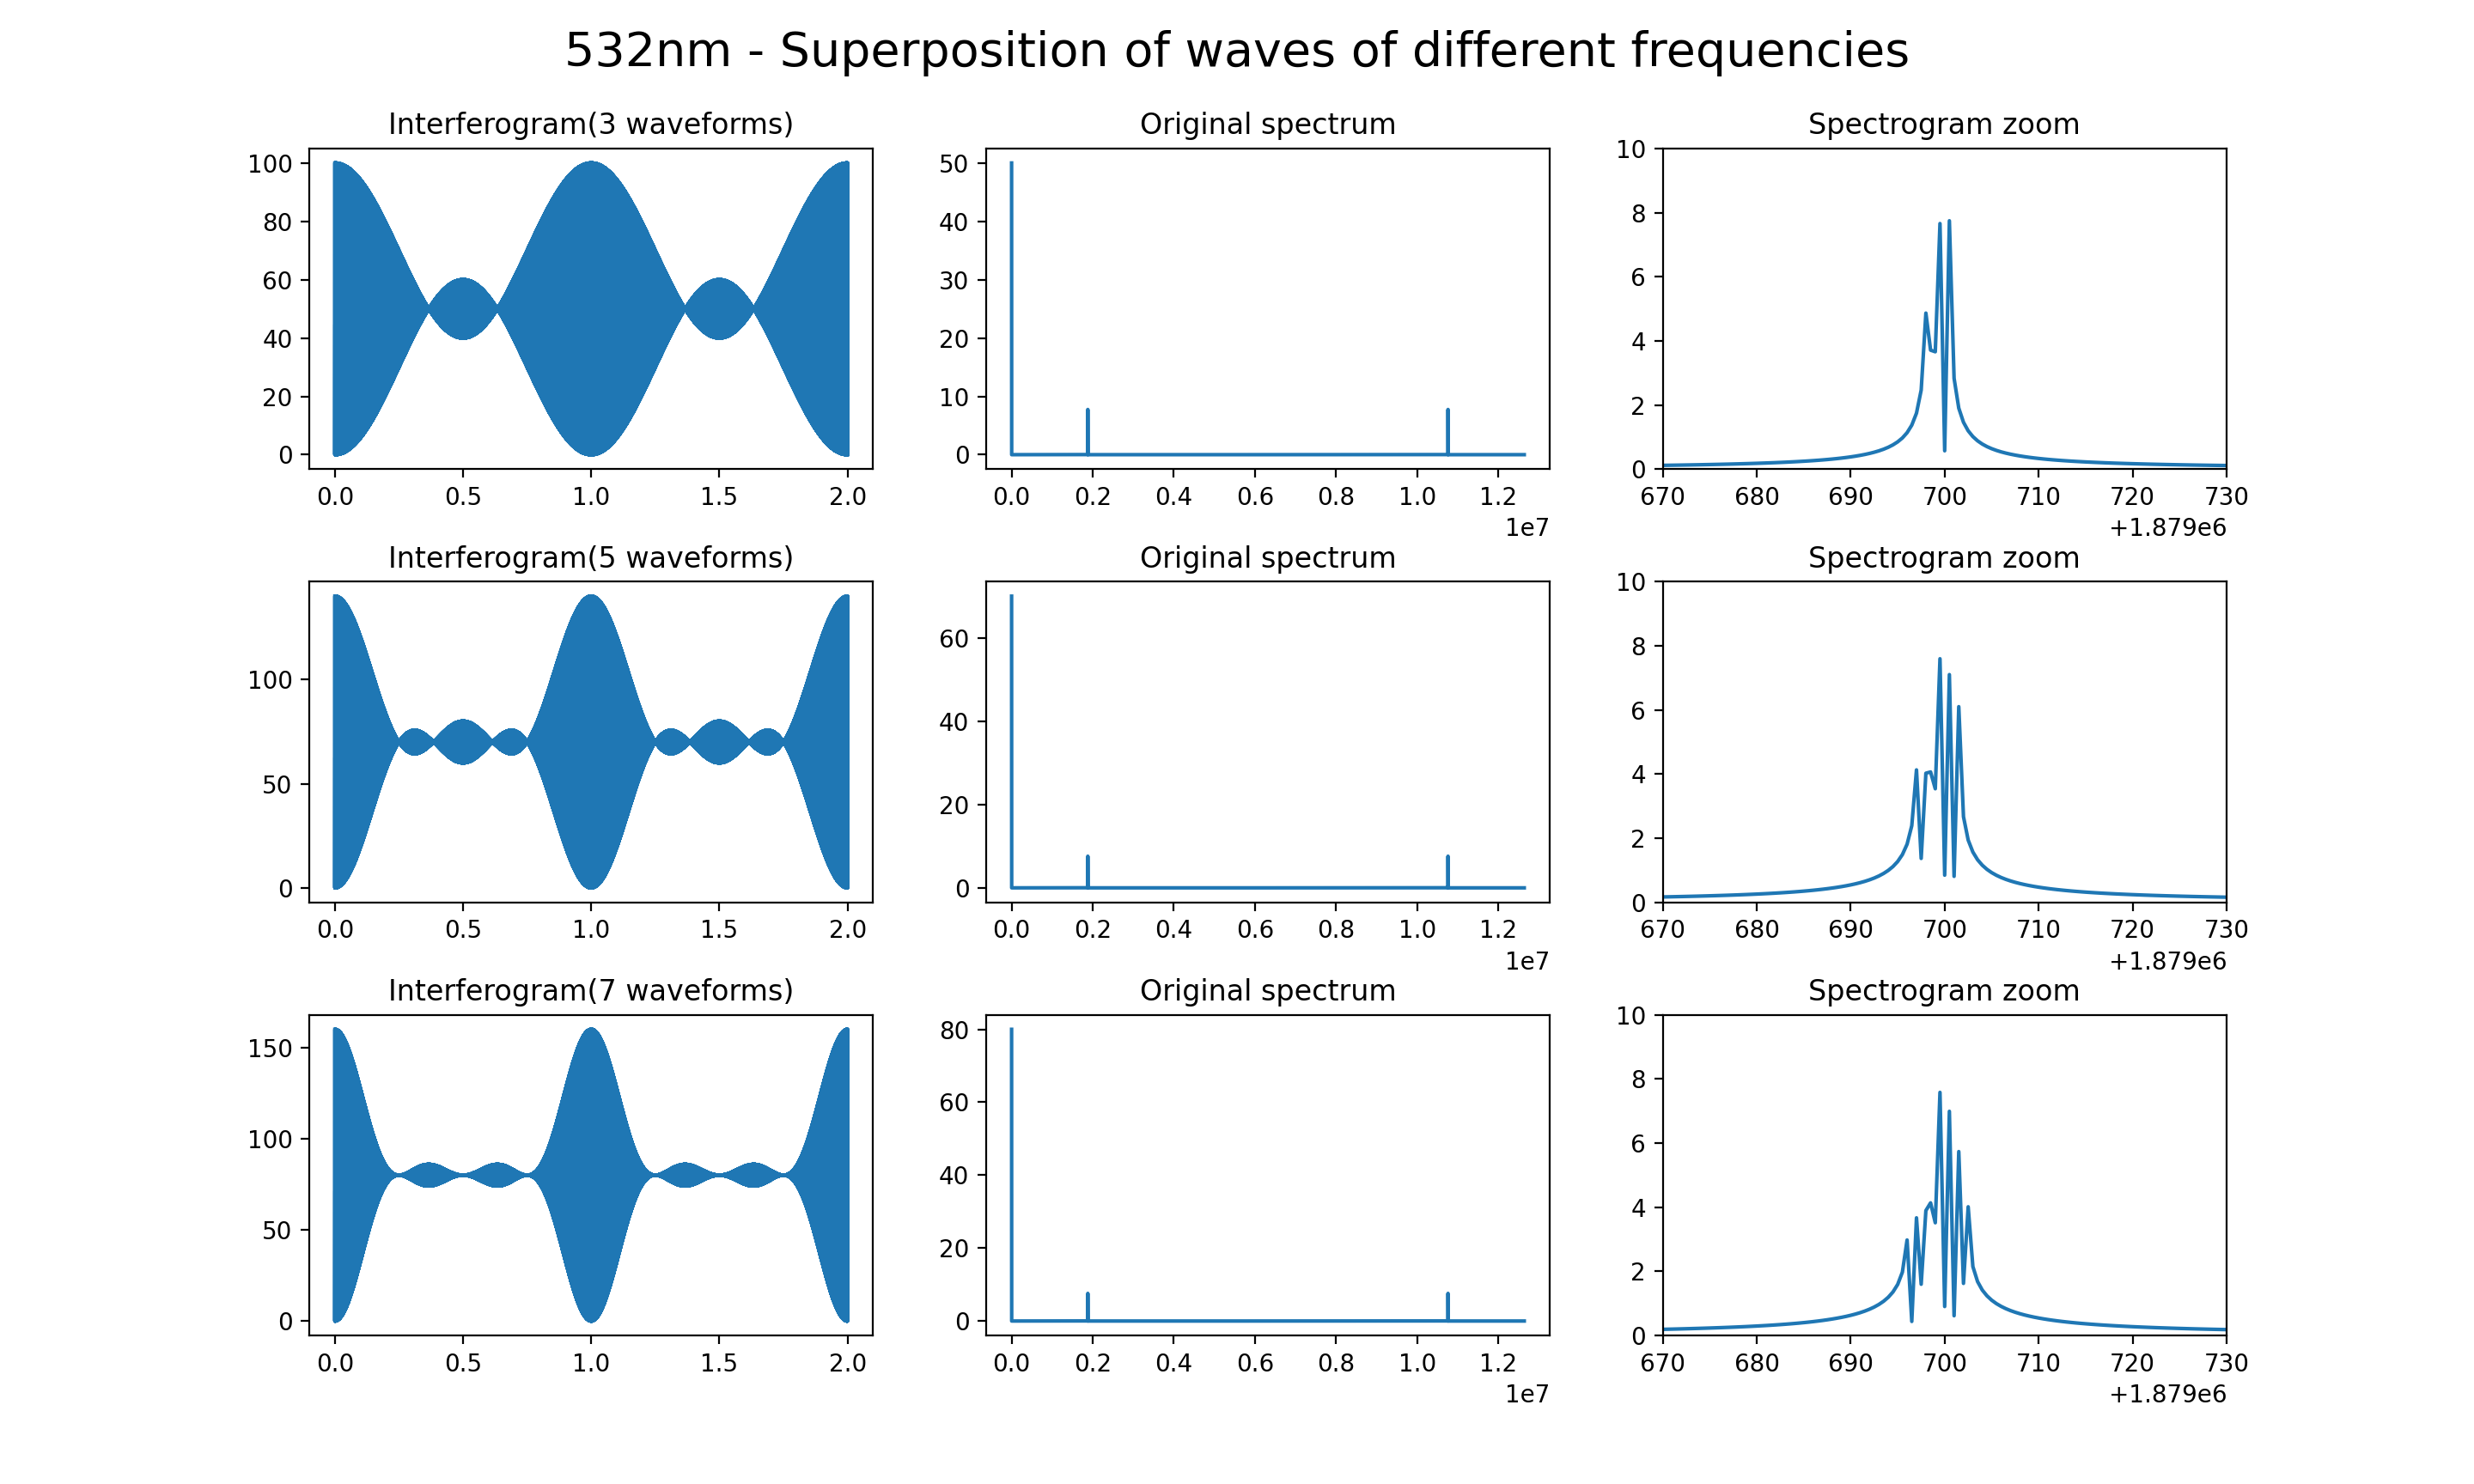
\includegraphics[width=0.5\textwidth]{pic25.png}}
    \caption{非单纵模 (多频) 激光输入FTS(情况16)}
    \label{pic25}
\end{figure}

本实验采样点个数的选取基于扫描长度Scan Length和采样间隔Sampling Interval的选择,具体公式为
\begin{align}
    N = \frac{Scan\;Length}{Sampling\;Interval}
\end{align}
从仿真图可以清楚的看出,当扫描长度不足2米时,快速傅立叶变换的精度没有达到预期效果,因此图\ref{pic10}-\ref{pic17}无法显示多个峰值;当扫描长度等于2米时,从图\ref{pic18}-\ref{pic25}可以清楚地看出来多个光干涉后的频谱。

\section{结语}
快速傅立叶算法可以实现信号从时域到频域的转变,方便科研工作者捕捉信号在时域上无法察觉的特征。本实验完成了利用Matlab或Python编程语言对多种频率正弦波的波形、其间的干涉图与光谱曲线进行仿真的工作。

\onecolumn
    \appendix[光谱曲线仿真代码]
{%\setmonofont[Mapping={}]{Consolas}
\begin{lstlisting}[language=python]
 import numpy as np
 import matplotlib.pyplot as plt
 from scipy.fftpack import fft, ifft
 from matplotlib.pylab import mpl
 from pylab import *

 class SuperpositionOfWaves(object):
    
     def __init__(self, lambda_center, sample_f, scan_length, sameAmplitude):
         # 设置是否等幅度
         self.sameAmplitude = sameAmplitude
         # 设置中心波长532nm
         self.lambda_center = lambda_center
         # 设置光速
         self.c = 3*10**8
         # 频率/HZ
         self.f = self.c/self.lambda_center
         # 频率间隔300MHz
         self.delta_f = 300*10**6
         # 干涉图采样间隔/m
         self.sample_f = sample_f
         # 扫描长度/m 
         self.scan_length = scan_length
         # 采样点个数
         self.N = int(self.scan_length/self.sample_f)
         # 光程差/m
         self.x = np.linspace(0,self.scan_length,int(self.scan_length/self.sample_f))
         # 设置采样频率
         self.fs = 1/self.sample_f*np.arange(self.N)/self.N
         # 设定强度频率/Hz
         self.f0 = self.f
         self.f1 = self.f-self.delta_f
         self.f2 = self.f+self.delta_f
         self.f3 = self.f-2*self.delta_f
         self.f4 = self.f+2*self.delta_f
         self.f5 = self.f-3*self.delta_f
         self.f6 = self.f+3*self.delta_f

         # 计算波长/m
         self.lambda0 = self.c/self.f0
         self.lambda1 = self.c/self.f1
         self.lambda2 = self.c/self.f2
         self.lambda3 = self.c/self.f3
         self.lambda4 = self.c/self.f4
         self.lambda5 = self.c/self.f5
         self.lambda6 = self.c/self.f6

         # 计算波数/m**(-1)
         self.sigma0=1/self.lambda0
         self.sigma1=1/self.lambda1
         self.sigma2=1/self.lambda2
         self.sigma3=1/self.lambda3
         self.sigma4=1/self.lambda4
         self.sigma5=1/self.lambda5
         self.sigma6=1/self.lambda6

         # 设定叠加的波
         if self.sameAmplitude:
             self.i0=1*(1+np.cos(2*np.pi*self.sigma0*self.x))
             self.i1=1*(1+np.cos(2*np.pi*self.sigma1*self.x))
             self.i2=1*(1+np.cos(2*np.pi*self.sigma2*self.x))
             self.i3=1*(1+np.cos(2*np.pi*self.sigma3*self.x))
             self.i4=1*(1+np.cos(2*np.pi*self.sigma4*self.x))
             self.i5=1*(1+np.cos(2*np.pi*self.sigma5*self.x))
             self.i6=1*(1+np.cos(2*np.pi*self.sigma6*self.x))
         else:
             self.i0=20*(1+np.cos(2*np.pi*self.sigma0*self.x))
             self.i1=15*(1+np.cos(2*np.pi*self.sigma1*self.x))
             self.i2=15*(1+np.cos(2*np.pi*self.sigma2*self.x))
             self.i3=10*(1+np.cos(2*np.pi*self.sigma3*self.x))
             self.i4=10*(1+np.cos(2*np.pi*self.sigma4*self.x))
             self.i5=5*(1+np.cos(2*np.pi*self.sigma5*self.x))
             self.i6=5*(1+np.cos(2*np.pi*self.sigma6*self.x))

         # 组合多种波
         self.ia = self.i0+self.i1+self.i2
         self.ib = self.i0+self.i1+self.i2+self.i3+self.i4
         self.ic = self.i0+self.i1+self.i2+self.i3+self.i4+self.i5+self.i6

     def drawInterferencePic(self):
         wave = [self.ia, self.ib, self.ic]
         for j in range(3):
             plt.subplot(3,3,3*j+1)
             plt.plot(self.x, wave[j])
             if j == 0:
                 plt.title("Interferogram(3 waveforms)")
             if j == 1:
                 plt.title("Interferogram(5 waveforms)")
             if j == 2:
                 plt.title("Interferogram(7 waveforms)")

             # 快速傅立叶变换
             y = np.abs(fft(wave[j]))/self.N
             plt.subplot(3,3,3*j+2)
             plt.plot(self.fs, y)
             plt.title("Original spectrum")

             # 放大后的频谱
             plt.subplot(3,3,3*j+3)
             plt.plot(self.fs, y)
             plt.title("Spectrogram zoom")
             if self.lambda_center < 632.8*10**(-9):
                 plt.xlim(1.87967*(10**6), 1.87973*(10**6))
             else:
                 plt.xlim(1.580255*(10**6), 1.5803*(10**6))
             if self.sameAmplitude:
                 plt.ylim(0, 1.5)
             else:
                 plt.ylim(0,10)
            
         if self.lambda_center < 632.8*10**(-9):
             plt.suptitle("532nm - Superposition of waves of different frequencies", fontsize = 20)  
         else:
             plt.suptitle("632.8nm - Superposition of waves of different frequencies", fontsize = 20)
        
         plt.subplots_adjust(left=0.125,
                            bottom=0.1, 
                            right=0.9, 
                            top=0.9, 
                            wspace=0.2, 
                            hspace=0.35)
         plt.show()

 a = SuperpositionOfWaves(sameAmplitude=False,lambda_center=532*10**(-9), sample_f=(632.8*10**(-9))/8, scan_length=2.0)
 a.drawInterferencePic()
\end{lstlisting}}

% \appendices
% \section{光谱曲线仿真代码}
% {%\setmonofont[Mapping={}]{Consolas}
% \begin{lstlisting}[language=python]
%  import numpy as np
%  import matplotlib.pyplot as plt
%  from scipy.fftpack import fft, ifft
%  from matplotlib.pylab import mpl
%  from pylab import *

%  class SuperpositionOfWaves(object):
    
%      def __init__(self, lambda_center, sample_f, scan_length, sameAmplitude):
%          # 设置是否等幅度
%          self.sameAmplitude = sameAmplitude
%          # 设置中心波长532nm
%          self.lambda_center = lambda_center
%          # 设置光速
%          self.c = 3*10**8
%          # 频率/HZ
%          self.f = self.c/self.lambda_center
%          # 频率间隔300MHz
%          self.delta_f = 300*10**6
%          # 干涉图采样间隔/m
%          self.sample_f = sample_f
%          # 扫描长度/m 
%          self.scan_length = scan_length
%          # 采样点个数
%          self.N = int(self.scan_length/self.sample_f)
%          # 光程差/m
%          self.x = np.linspace(0,self.scan_length,int(self.scan_length/self.sample_f))
%          # 设置采样频率
%          self.fs = 1/self.sample_f*np.arange(self.N)/self.N
%          # 设定强度频率/Hz
%          self.f0 = self.f
%          self.f1 = self.f-self.delta_f
%          self.f2 = self.f+self.delta_f
%          self.f3 = self.f-2*self.delta_f
%          self.f4 = self.f+2*self.delta_f
%          self.f5 = self.f-3*self.delta_f
%          self.f6 = self.f+3*self.delta_f

%          # 计算波长/m
%          self.lambda0 = self.c/self.f0
%          self.lambda1 = self.c/self.f1
%          self.lambda2 = self.c/self.f2
%          self.lambda3 = self.c/self.f3
%          self.lambda4 = self.c/self.f4
%          self.lambda5 = self.c/self.f5
%          self.lambda6 = self.c/self.f6

%          # 计算波数/m**(-1)
%          self.sigma0=1/self.lambda0
%          self.sigma1=1/self.lambda1
%          self.sigma2=1/self.lambda2
%          self.sigma3=1/self.lambda3
%          self.sigma4=1/self.lambda4
%          self.sigma5=1/self.lambda5
%          self.sigma6=1/self.lambda6

%          # 设定叠加的波
%          if self.sameAmplitude:
%              self.i0=1*(1+np.cos(2*np.pi*self.sigma0*self.x))
%              self.i1=1*(1+np.cos(2*np.pi*self.sigma1*self.x))
%              self.i2=1*(1+np.cos(2*np.pi*self.sigma2*self.x))
%              self.i3=1*(1+np.cos(2*np.pi*self.sigma3*self.x))
%              self.i4=1*(1+np.cos(2*np.pi*self.sigma4*self.x))
%              self.i5=1*(1+np.cos(2*np.pi*self.sigma5*self.x))
%              self.i6=1*(1+np.cos(2*np.pi*self.sigma6*self.x))
%          else:
%              self.i0=20*(1+np.cos(2*np.pi*self.sigma0*self.x))
%              self.i1=15*(1+np.cos(2*np.pi*self.sigma1*self.x))
%              self.i2=15*(1+np.cos(2*np.pi*self.sigma2*self.x))
%              self.i3=10*(1+np.cos(2*np.pi*self.sigma3*self.x))
%              self.i4=10*(1+np.cos(2*np.pi*self.sigma4*self.x))
%              self.i5=5*(1+np.cos(2*np.pi*self.sigma5*self.x))
%              self.i6=5*(1+np.cos(2*np.pi*self.sigma6*self.x))

%          # 组合多种波
%          self.ia = self.i0+self.i1+self.i2
%          self.ib = self.i0+self.i1+self.i2+self.i3+self.i4
%          self.ic = self.i0+self.i1+self.i2+self.i3+self.i4+self.i5+self.i6

%      def drawInterferencePic(self):
%          wave = [self.ia, self.ib, self.ic]
%          for j in range(3):
%              plt.subplot(3,3,3*j+1)
%              plt.plot(self.x, wave[j])
%              if j == 0:
%                  plt.title("Interferogram(3 waveforms)")
%              if j == 1:
%                  plt.title("Interferogram(5 waveforms)")
%              if j == 2:
%                  plt.title("Interferogram(7 waveforms)")

%              # 快速傅立叶变换
%              y = np.abs(fft(wave[j]))/self.N
%              plt.subplot(3,3,3*j+2)
%              plt.plot(self.fs, y)
%              plt.title("Original spectrum")

%              # 放大后的频谱
%              plt.subplot(3,3,3*j+3)
%              plt.plot(self.fs, y)
%              plt.title("Spectrogram zoom")
%              if self.lambda_center < 632.8*10**(-9):
%                  plt.xlim(1.87967*(10**6), 1.87973*(10**6))
%              else:
%                  plt.xlim(1.580255*(10**6), 1.5803*(10**6))
%              if self.sameAmplitude:
%                  plt.ylim(0, 1.5)
%              else:
%                  plt.ylim(0,10)
            
%          if self.lambda_center < 632.8*10**(-9):
%              plt.suptitle("532nm - Superposition of waves of different frequencies", fontsize = 20)  
%          else:
%              plt.suptitle("632.8nm - Superposition of waves of different frequencies", fontsize = 20)
        
%          plt.subplots_adjust(left=0.125,
%                             bottom=0.1, 
%                             right=0.9, 
%                             top=0.9, 
%                             wspace=0.2, 
%                             hspace=0.35)
%          plt.show()

%  a = SuperpositionOfWaves(sameAmplitude=False,lambda_center=532*10**(-9), sample_f=(632.8*10**(-9))/8, scan_length=2.0)
%  a.drawInterferencePic()
% \end{lstlisting}}

\end{document}
